%========================================
% Cnot 1.7 — main.tex
%========================================
%\documentclass[14pt,oneside,a4paper]{book}
\documentclass[10pt,oneside]{extbook} % KDP 6x9: il formato pagina lo imposta geometry

% ---------- Encoding & lingua ----------
\usepackage[T1]{fontenc}
\usepackage[utf8]{inputenc} % con XeLaTeX/LuaLaTeX non serve
\usepackage[italian]{babel}
\usepackage{microtype}
\usepackage{libertinus}
\usepackage{verbatim}


% ---------- Impaginazione ----------
% KDP 6 x 9 in = 152.4 x 228.6 mm, SENZA bleed
% Se in KDP hai selezionato 152.4 x 228.6 mm, il PDF interno deve avere esattamente questa pagina.
\usepackage[
  paperwidth=152.4mm,
  paperheight=228.6mm,
  inner=18mm,
  outer=14mm,
  top=15mm,
  bottom=18mm,
  headheight=22pt,
  headsep=5mm,
  includehead
]{geometry}
\usepackage{setspace}
\onehalfspacing

% ---------- Grafica & colori ----------
\usepackage{fancyvrb}
\usepackage[most]{tcolorbox}
\usepackage{graphicx}
\usepackage{xcolor}
\usepackage{float}
\graphicspath{{media/}{figures/}{images/}{gis}}

% ---------- Tipografia ----------
\usepackage{csquotes}
\usepackage{booktabs}
\usepackage{array}

% ---------- Riferimenti & PDF ----------
\usepackage{hyperref}
\hypersetup{
  pdftitle={Cnot 1.7},
  pdfauthor={Edizioni Tradizionali},
  pdfsubject={Romanzo / Progetto Cnot 1.7},
  pdfkeywords={Cnot 1.7, narrativa, Edizioni Tradizionali},
  colorlinks=true,
  linkcolor=black,
  citecolor=black,
  urlcolor=black
}
\usepackage{bookmark} % segnalibri robusti

% ---------- Intestazioni/Piè di pagina ----------
\usepackage{fancyhdr}
\pagestyle{fancy}
\fancyhf{}
\fancyhead[LE,RO]{\thepage}
\fancyhead[LO]{\nouppercase{\rightmark}}
\fancyhead[RE]{\nouppercase{\leftmark}}

% ---------- Titoli ----------
\usepackage{titlesec}
\usepackage{xcolor}
% Capitolo compatto e più piccolo

% Colore sobrio e “editoriale” (modificalo a gusto)
\definecolor{ChapterColor}{HTML}{2A3F5F} % blu ardesia
%\definecolor{ChapterColor}{HTML}{3A4A3F} % verde-grigio alternativo
%\definecolor{ChapterColor}{HTML}{5A4B41} % seppia caldo

% Stile capitolo numerato
\titleformat{\chapter}[display]
  {\filcenter\bfseries\Large\color{ChapterColor}} % centro + peso + size + colore
  {\textsc{\MakeUppercase{Capitolo} \thechapter}} % riga sopra: “Capitolo N” in small caps
  {0.5ex}                                         % spazio tra label e titolo
  {\filcenter}                                     % il titolo vero e proprio, centrato
  [\vspace{0.75ex}\color{ChapterColor}\rule{2.5cm}{0.6pt}] % filetto finale discreto

%\titleformat{\chapter}[display]
 % {\bfseries\Large}        % <- dimensione titolo (cambia \Large in \large o \normalsize)
 % {\filright\small\MakeUppercase{\chaptername}\ \thechapter} % riga “Capitolo N”
 % {1ex}                    % spazio tra numero e titolo
 % {\filright}              % allineamento del titolo
%\titlespacing*{\chapter}{0pt}{2ex}{2ex}  % margini/spacing: sinistra, prima, dopo


% ---------- Comandi utili ----------
\newcommand{\CCBYSA}{\includegraphics[height=1.2em]{cc-by-sa.png}} % opzionale

\newcommand{\separatore}{%
  \par
  \begin{center}
    {\Large $\sim\!\!\sim\!\!\sim\ \ast\ \sim\!\!\sim\!\!\sim$}
  \end{center}
  \par
}


\definecolor{terminalblack}{HTML}{101410}
\definecolor{phosphorgreen}{HTML}{66FF66}

\newtcblisting{terminalbox}{
  listing only,
  colback=terminalblack,
  colframe=terminalblack,
  arc=1mm,
  boxrule=0pt,
  left=8pt,
  right=8pt,
  top=7pt,
  bottom=7pt,
  listing options={
    basicstyle=\ttfamily\small\bfseries\color{phosphorgreen},
    breaklines=true,
    columns=fixed,
    keepspaces=true,
    showstringspaces=false
  }
}

\definecolor{phosphoramber}{HTML}{D39A2E}
\definecolor{mygreen}{HTML}{8DBB47}

\newtcblisting{terminalbox_gi}{
  listing only,
  colback=mygreen,
  colframe=mygreen,
  arc=2mm,
  boxrule=0pt,
  left=6pt,
  right=6pt,
  top=6pt,
  bottom=6pt,
  listing options={
    basicstyle=\ttfamily\small\color{black},
    breaklines=true,
    columns=fullflexible
  }
}

\newtcblisting{terminalbox_k}{
  listing only,
  colback=black,
  colframe=black,
  arc=2mm,
  boxrule=0pt,
  left=6pt,
  right=6pt,
  top=6pt,
  bottom=6pt,
  listing options={
    basicstyle=\ttfamily\small\color{green!70!white},
    breaklines=true,
    columns=fullflexible
  }
}

\newtcblisting{terminalbox_ambra}{
  listing only,
  colback=phosphoramber,
  colframe=phosphoramber,
  arc=2mm,
  boxrule=0pt,
  left=6pt,
  right=6pt,
  top=6pt,
  bottom=6pt,
  listing options={
    basicstyle=\ttfamily\small\color{black},
    breaklines=true,
    columns=fullflexible
  }
}

% ---------- Dati del libro ----------
\title{\textbf{Cnot 1.7}}
\author{Edizioni Tradizionali}
%\date{\today}

% ---------- (Opzionale) includeonly per compilazioni rapide ----------
% \includeonly{chapters/frontespizio,chapters/premessa,chapters/prologo,chapters/capitolo01}

\begin{document}

%========================================
% Front matter
%========================================
\frontmatter
\maketitle % Se preferisci un frontespizio personalizzato, commenta questa riga e usa chapters/frontespizio.tex

% Frontespizio personalizzato (opzionale, sostituisce \maketitle)
% chapters/frontespizio.tex
\clearpage
\thispagestyle{empty}

\begin{titlepage}
  \centering
  \vspace*{22mm}

  {\Huge\bfseries Cnot~1.7\par}

  \vspace{8mm}
  {\Large Francesco Sisini\par}

  \vspace{4mm}
  {\normalsize Illustrazioni a cura di Annalisa Pazzi\par}

  \vfill

  
\includegraphics[width=0.22\linewidth]{media/edizioni tradizionali.png}\par


\end{titlepage}


% Indice (se lo vuoi all’inizio)
\tableofcontents
\cleardoublepage


%========================================
% Corpo del libro
%========================================
\mainmatter

% Pagine prima del prologo senza numero stampato
\pagenumbering{gobble}

%%%%%%%%%%%%%%%%%%%%%%%%%%%%%%%%%%%%%%%%%%%%%%%%%%%%%%%%%%%%%%%%
%
%       PASSO 1
%
%%%%%%%%%%%%%%%%%%%%%%%%%%%%%%%%%%%%%%%%%%%%%%%%%%%%%%%%%%%%%%%%
\clearpage
\thispagestyle{empty}
\pagecolor{black}
\color{white}

\vspace*{\fill}

\begin{center}
\Large
A metà del ventunesimo secolo,\\[1em]
l’Europa è scivolata in una guerra invisibile e sottile.\\[1em]
\end{center}
\vspace*{\fill}
\clearpage

\begin{figure}[H]
  \centering
  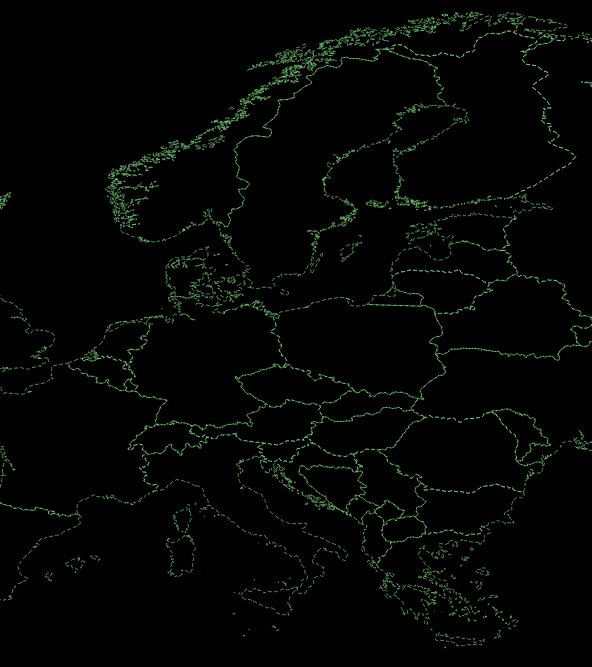
\includegraphics[width=0.9\linewidth]{gis/e1.png}
  
\end{figure}


%%%%%%%%%%%%%%%%%%%%%%%%%%%%%%%%%%%%%%%%%%%%%%%%%%%%%%%%%%%%%%%%
%
%       PASSO 2
%
%%%%%%%%%%%%%%%%%%%%%%%%%%%%%%%%%%%%%%%%%%%%%%%%%%%%%%%%%%%%%%%%
\clearpage
\thispagestyle{empty}
\pagecolor{black}
\color{white}

\vspace*{\fill}

\begin{center}
\Large
La sovranità degli stati è limitata da interessi inconoscibili.\\[1em]

\end{center}
\vspace*{\fill}
\clearpage

\begin{figure}[H]
  \centering
  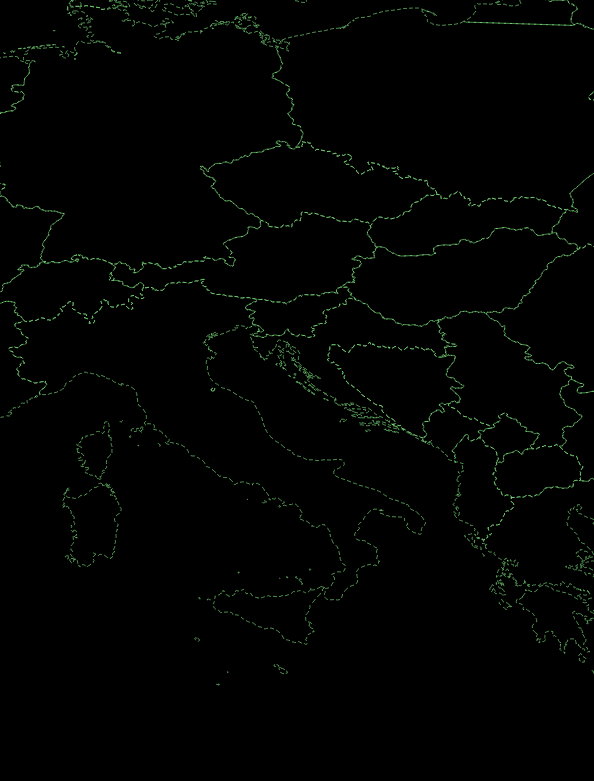
\includegraphics[width=0.9\linewidth]{gis/e2.png}
  
\end{figure}
\clearpage

%%%%%%%%%%%%%%%%%%%%%%%%%%%%%%%%%%%%%%%%%%%%%%%%%%%%%%%%%%%%%%%%
%
%       PASSO 3
%
%%%%%%%%%%%%%%%%%%%%%%%%%%%%%%%%%%%%%%%%%%%%%%%%%%%%%%%%%%%%%%%%
\clearpage
\thispagestyle{empty}
\pagecolor{black}
\color{white}

\vspace*{\fill}

\begin{center}
\Large
Il concetto di nazione proprio del XX secolo non è più attuale.\\[1em]

\end{center}
\vspace*{\fill}
\clearpage

\begin{figure}[H]
  \centering
  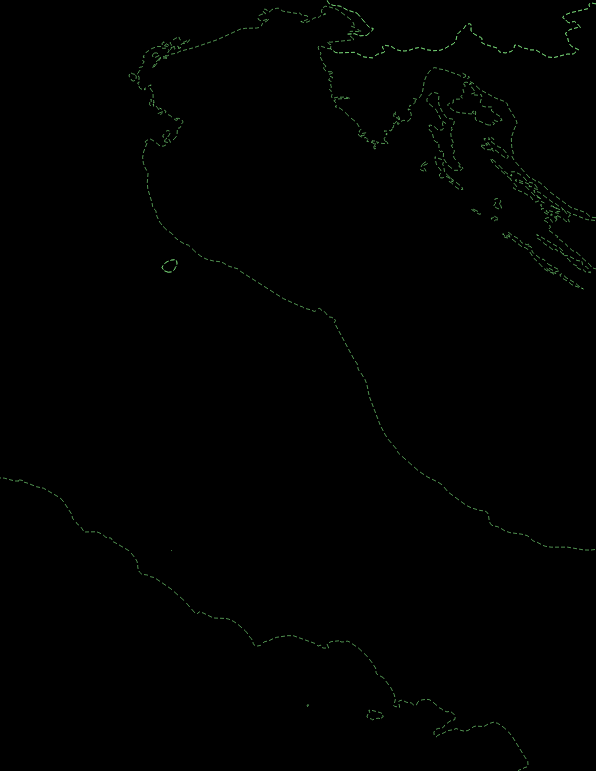
\includegraphics[width=0.9\linewidth]{gis/e3.png}
  
\end{figure}
\clearpage



%%%%%%%%%%%%%%%%%%%%%%%%%%%%%%%%%%%%%%%%%%%%%%%%%%%%%%%%%%%%%%%%
%
%       PASSO 4
%
%%%%%%%%%%%%%%%%%%%%%%%%%%%%%%%%%%%%%%%%%%%%%%%%%%%%%%%%%%%%%%%%
\clearpage
\thispagestyle{empty}
\pagecolor{black}
\color{white}

\vspace*{\fill}

\begin{center}
\Large
La vita e le relazioni si sviluppano su due piani paralleli, uno locale, prossimo, fisicamente vicino.\\[1em]

\end{center}
\vspace*{\fill}
\clearpage

\begin{figure}[H]
  \centering
  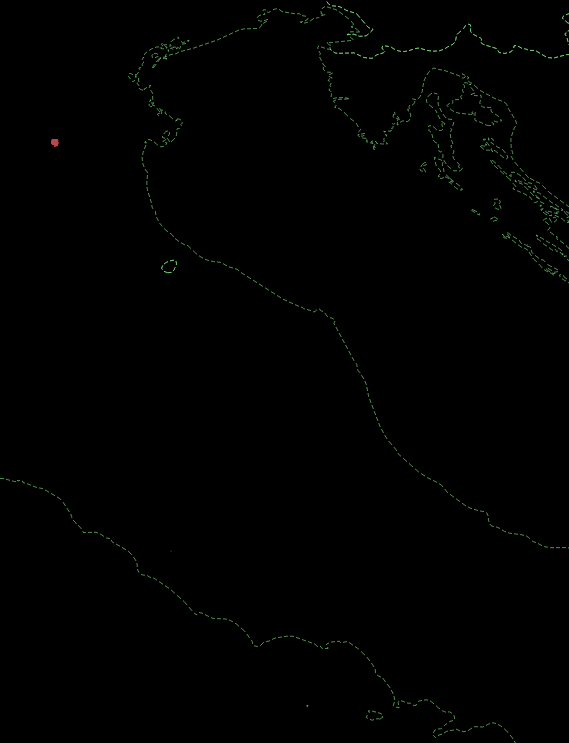
\includegraphics[width=0.9\linewidth]{gis/e4.png}
  
\end{figure}
\clearpage



%%%%%%%%%%%%%%%%%%%%%%%%%%%%%%%%%%%%%%%%%%%%%%%%%%%%%%%%%%%%%%%%
%
%       PASSO 5
%
%%%%%%%%%%%%%%%%%%%%%%%%%%%%%%%%%%%%%%%%%%%%%%%%%%%%%%%%%%%%%%%%
\clearpage
\thispagestyle{empty}
\pagecolor{black}
\color{white}

\vspace*{\fill}

\begin{center}
\Large
e uno affine, dove contano le reciproche distanze e non il centro\\[1em]

\end{center}
\vspace*{\fill}
\clearpage

\begin{figure}[H]
  \centering
  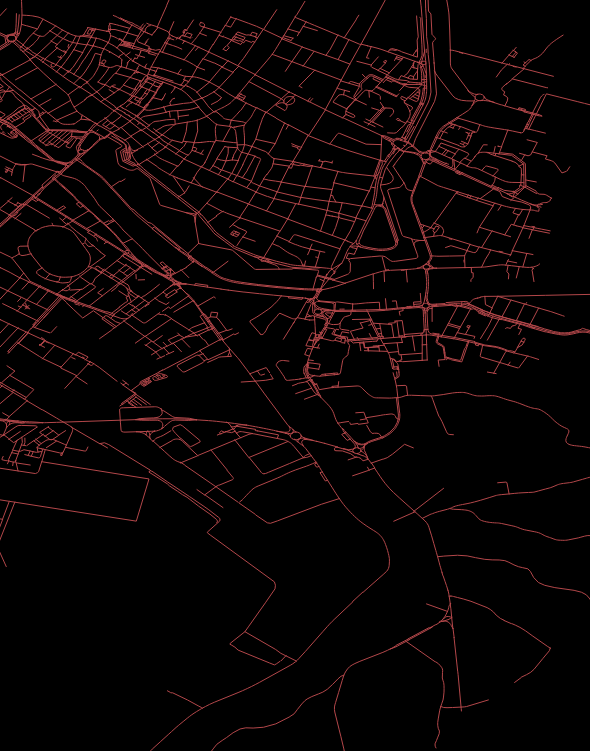
\includegraphics[width=0.9\linewidth]{gis/e5.png}
  
\end{figure}
\clearpage



%%%%%%%%%%%%%%%%%%%%%%%%%%%%%%%%%%%%%%%%%%%%%%%%%%%%%%%%%%%%%%%%
%
%       PASSO 5
%
%%%%%%%%%%%%%%%%%%%%%%%%%%%%%%%%%%%%%%%%%%%%%%%%%%%%%%%%%%%%%%%%
\clearpage
\thispagestyle{empty}
\pagecolor{black}
\color{white}

\vspace*{\fill}

\begin{center}
\Large
Le abtazioni convenzionali sono diventate difficilmente sostenibili\\[1em]

\end{center}
\vspace*{\fill}
\clearpage

\begin{figure}[H]
  \centering
  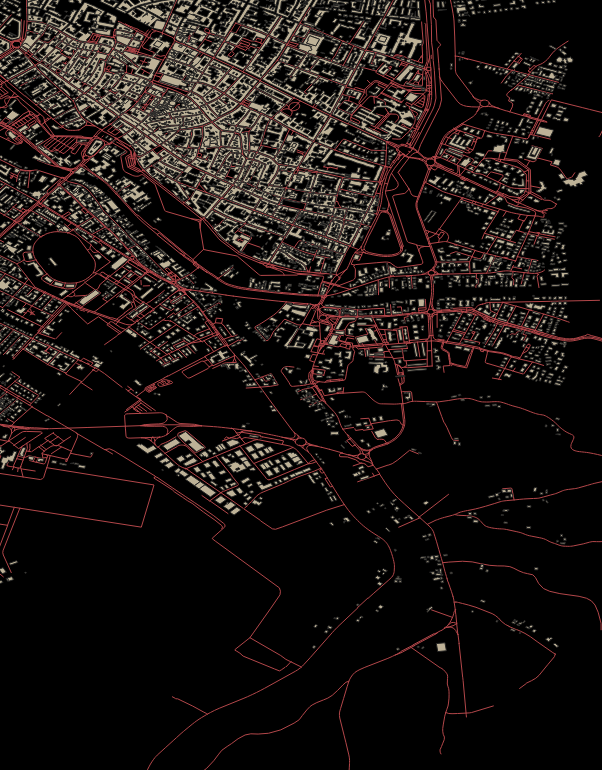
\includegraphics[width=0.9\linewidth]{gis/e6.png}
  
\end{figure}
\clearpage


%%%%%%%%%%%%%%%%%%%%%%%%%%%%%%%%%%%%%%%%%%%%%%%%%%%%%%%%%%%%%%%%
%
%       PASSO 7
%
%%%%%%%%%%%%%%%%%%%%%%%%%%%%%%%%%%%%%%%%%%%%%%%%%%%%%%%%%%%%%%%%
\clearpage
\thispagestyle{empty}
\pagecolor{black}
\color{white}

\vspace*{\fill}

\begin{center}
\Large
I velivoli hanno preso progressivamente il posto dei veicoli porando ad un progressivo abbandono della cura delle strade.\\[1em]

\end{center}
\vspace*{\fill}
\clearpage

\begin{figure}[H]
  \centering
  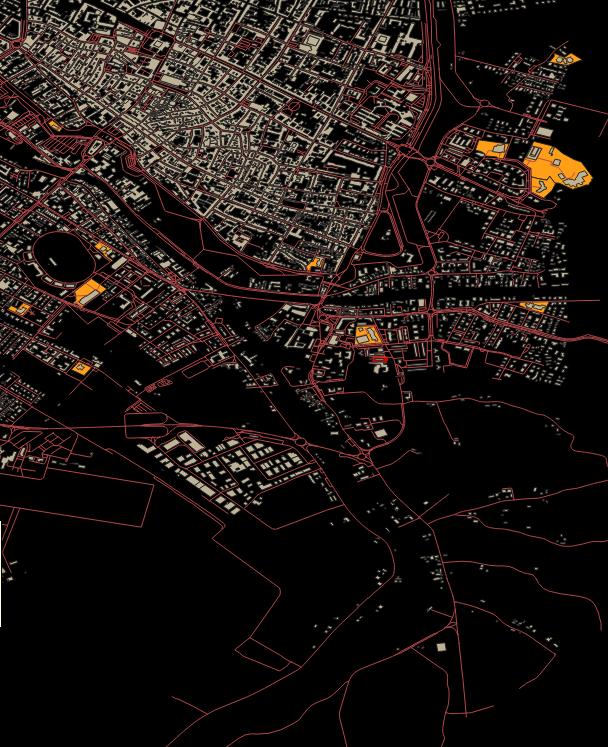
\includegraphics[width=0.9\linewidth]{gis/e7.png}
  
\end{figure}
\clearpage



%%%%%%%%%%%%%%%%%%%%%%%%%%%%%%%%%%%%%%%%%%%%%%%%%%%%%%%%%%%%%%%%
%
%       PASSO 8
%
%%%%%%%%%%%%%%%%%%%%%%%%%%%%%%%%%%%%%%%%%%%%%%%%%%%%%%%%%%%%%%%%
\clearpage
\thispagestyle{empty}
\pagecolor{black}
\color{white}

\vspace*{\fill}

\begin{center}
\Large
La vegetazione ha occupato i luoghi che un tempo erano abitati, \\[1em]

\end{center}
\vspace*{\fill}
\clearpage

\begin{figure}[H]
  \centering
  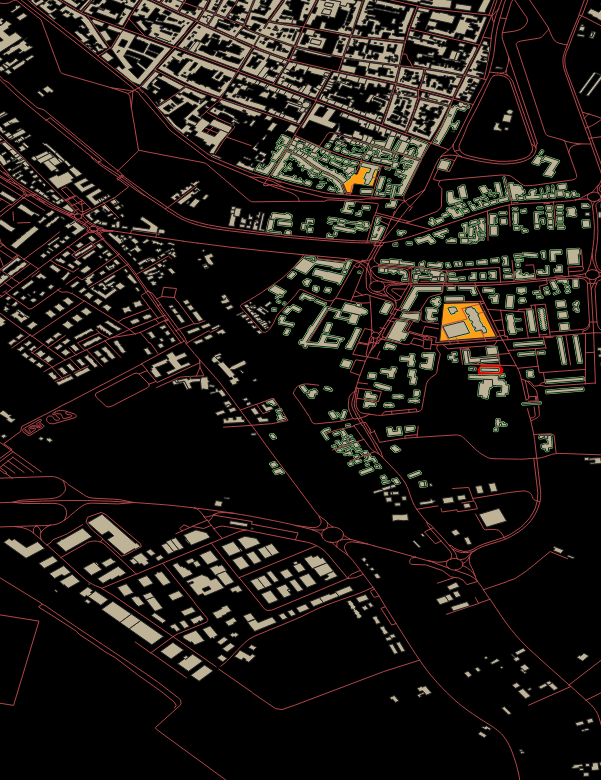
\includegraphics[width=0.9\linewidth]{gis/e8.png}
  
\end{figure}
\clearpage



%%%%%%%%%%%%%%%%%%%%%%%%%%%%%%%%%%%%%%%%%%%%%%%%%%%%%%%%%%%%%%%%
%
%       PASSO 9
%
%%%%%%%%%%%%%%%%%%%%%%%%%%%%%%%%%%%%%%%%%%%%%%%%%%%%%%%%%%%%%%%%
\clearpage
\thispagestyle{empty}
\pagecolor{black}
\color{white}

\vspace*{\fill}

\begin{center}
\Large
gli emarginati sociali vivono dove prima era loro proibito \\[1em]

\end{center}
\vspace*{\fill}
\clearpage

\begin{figure}[H]
  \centering
  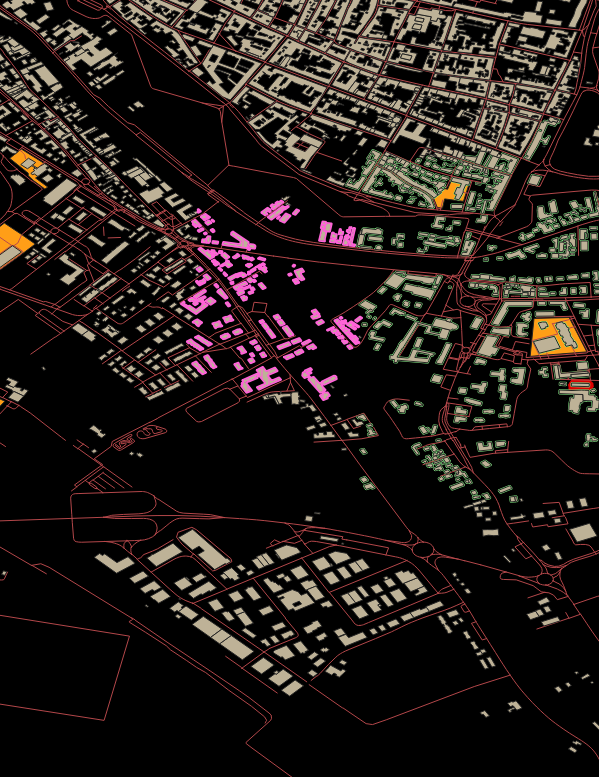
\includegraphics[width=0.9\linewidth]{gis/e9.png}
  
\end{figure}
\clearpage


%%%%%%%%%%%%%%%%%%%%%%%%%%%%%%%%%%%%%%%%%%%%%%%%%%%%%%%%%%%%%%%%
%
%       PASSO 10
%
%%%%%%%%%%%%%%%%%%%%%%%%%%%%%%%%%%%%%%%%%%%%%%%%%%%%%%%%%%%%%%%%
\clearpage
\thispagestyle{empty}
\pagecolor{black}
\color{white}

\vspace*{\fill}

\begin{center}
\Large
gli edifici abbandonati sono diventati la casa di alcuni, mentre per altri \\[1em]

\end{center}
\vspace*{\fill}
\clearpage

\begin{figure}[H]
  \centering
  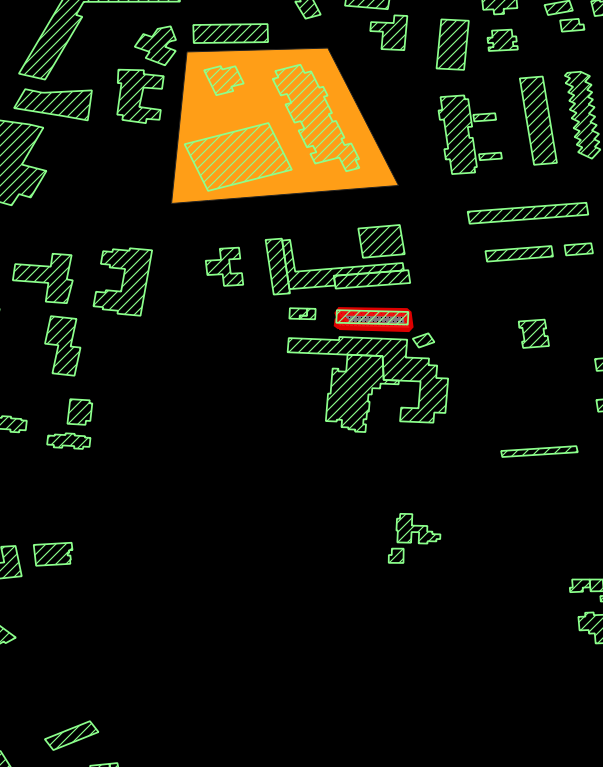
\includegraphics[width=0.9\linewidth]{gis/e10.png}
  
\end{figure}
\clearpage


%%%%%%%%%%%%%%%%%%%%%%%%%%%%%%%%%%%%%%%%%%%%%%%%%%%%%%%%%%%%%%%%
%
%       PASSO 11
%
%%%%%%%%%%%%%%%%%%%%%%%%%%%%%%%%%%%%%%%%%%%%%%%%%%%%%%%%%%%%%%%%
\clearpage
\thispagestyle{empty}
\pagecolor{black}
\color{white}

\vspace*{\fill}

\begin{center}
\Large
inconsapevoli di chi li osserva,  \\[1em]

\end{center}
\vspace*{\fill}
\clearpage

\begin{figure}[H]
  \centering
  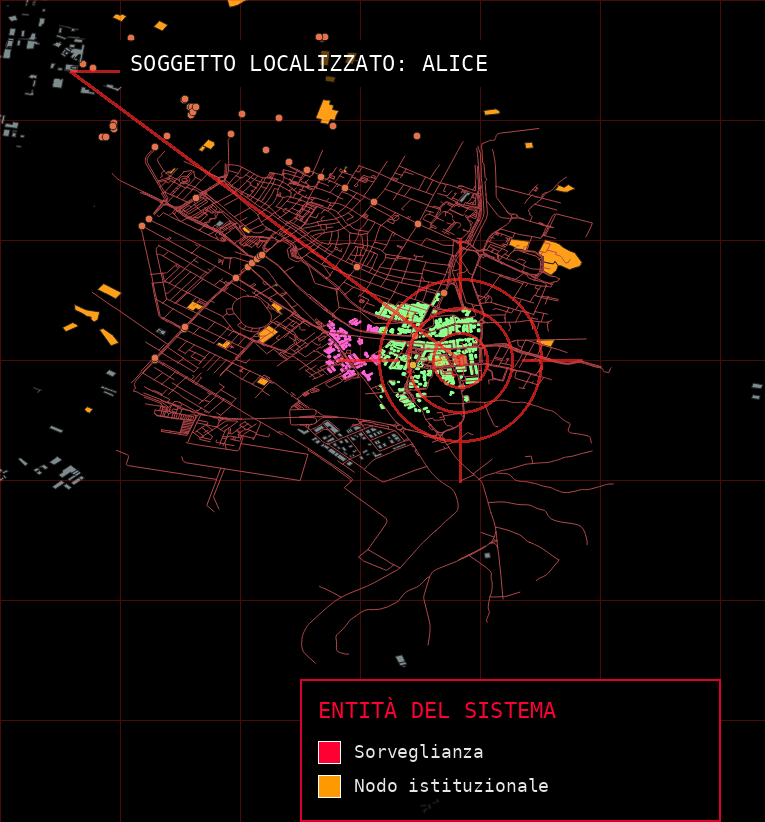
\includegraphics[width=0.9\linewidth]{gis/ferrara_overlay.png}
  
\end{figure}
\clearpage


%%%%%%%%%%%%%%%%%%%%%%%%%%%%%%%%%%%%%%%%%%%%%%%%%%%%%%%%%%%%%%%%
%
%       PASSO 12
%
%%%%%%%%%%%%%%%%%%%%%%%%%%%%%%%%%%%%%%%%%%%%%%%%%%%%%%%%%%%%%%%%
\clearpage
\thispagestyle{empty}
\pagecolor{black}
\color{white}

\vspace*{\fill}

\begin{center}
\Large
la vita continua come prima... \\[1em]

\end{center}
\vspace*{\fill}
\clearpage

\begin{figure}[H]
  \centering
  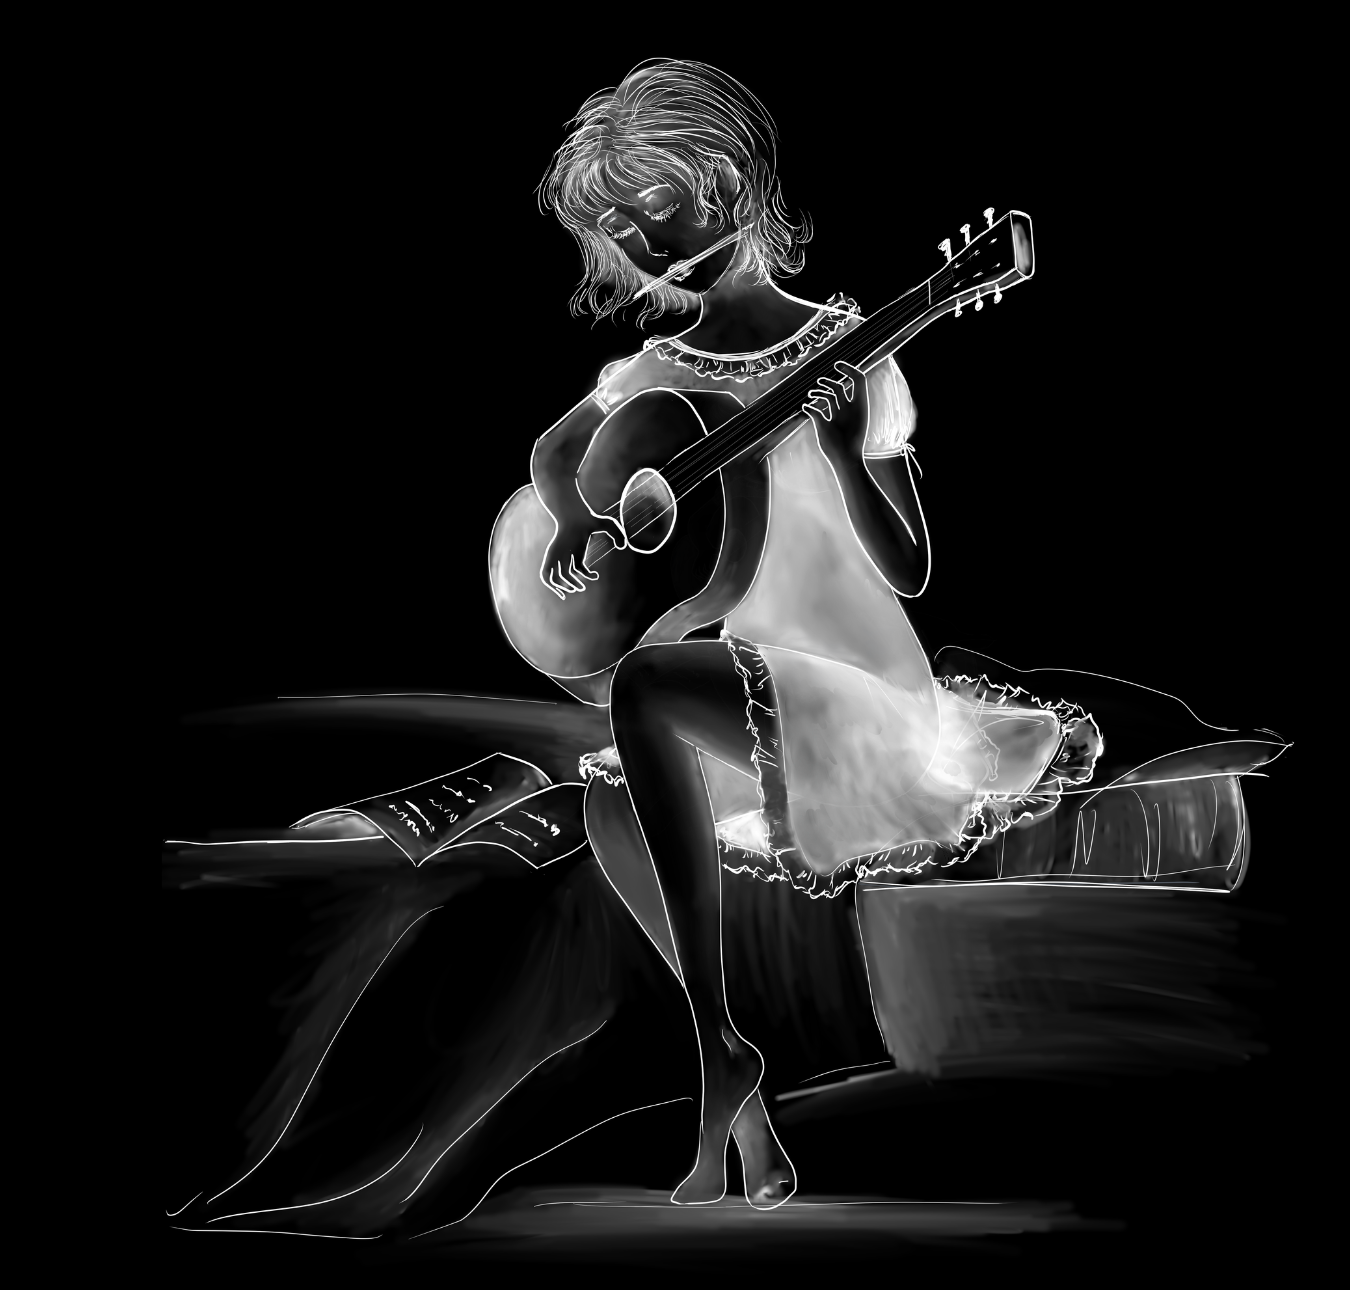
\includegraphics[width=0.9\linewidth]{alice bianca.png}
  
\end{figure}
\clearpage




\nopagecolor
\color{black}

% --- domanda ---
\clearpage
\thispagestyle{empty}

\vspace*{\fill}

\begin{center}
{\Large $\sim\!\!\sim\!\!\sim\ \ast\ \sim\!\!\sim\!\!\sim$}
\vspace{2em}

\begin{minipage}{0.78\textwidth}
\itshape

L'amore di una donna per un uomo è più forte del suo desiderio di affermazione personale?
Le scelte ideologiche si applicano a tutte le scale o solo ad alcune?
La libertà paga o paghi per averla?

\medskip

Tieni presente queste tre domande mentre leggi il mio resoconto di questa avventura
che vede unite Laura e Caterina. Ho cercato in ogni modo di non condizionare il tuo
giudizio; ti chiedo in cambio di pensarmi quando avrai finito di leggerlo, di farlo
con intensità, in modo che l'universo abbia le tue risposte.

\end{minipage}
\end{center}

\vspace*{\fill}

\clearpage


% Da qui parte la numerazione editoriale: Prologo = pagina 1
\cleardoublepage
% --- prologo ---
% chapters/prologo.tex
\cleardoublepage

\chapter*{Prologo. Lacrime in cameretta}
\markboth{Prologo}{Prologo}



Alice resta chiusa in camera, al riparo, senza che nessuno possa vedere, minimizzare, giudicare.\\
Prende un quaderno, una penna e la chitarra che le ha regalato suo padre dopo il saggio di flauto.\\

Non l'ha studiata molto, ma conosce gli accordi maggiori e quelli minori, e qualcosa su quelli di  settima nona. A quanto pare sa anche come si scrive una canzone partendo da un testo; non uno di quelli più o meno scontati che si trovano in streaming, ma un testo che sa parlare a una sola persona, che sa avvicinarla con delicatezza, farle aprire le porte del cuore per poi piantarci un coltello. \\
Già, proprio come ha fatto Caterina con lei.

\begin{figure}[H]
  \centering
  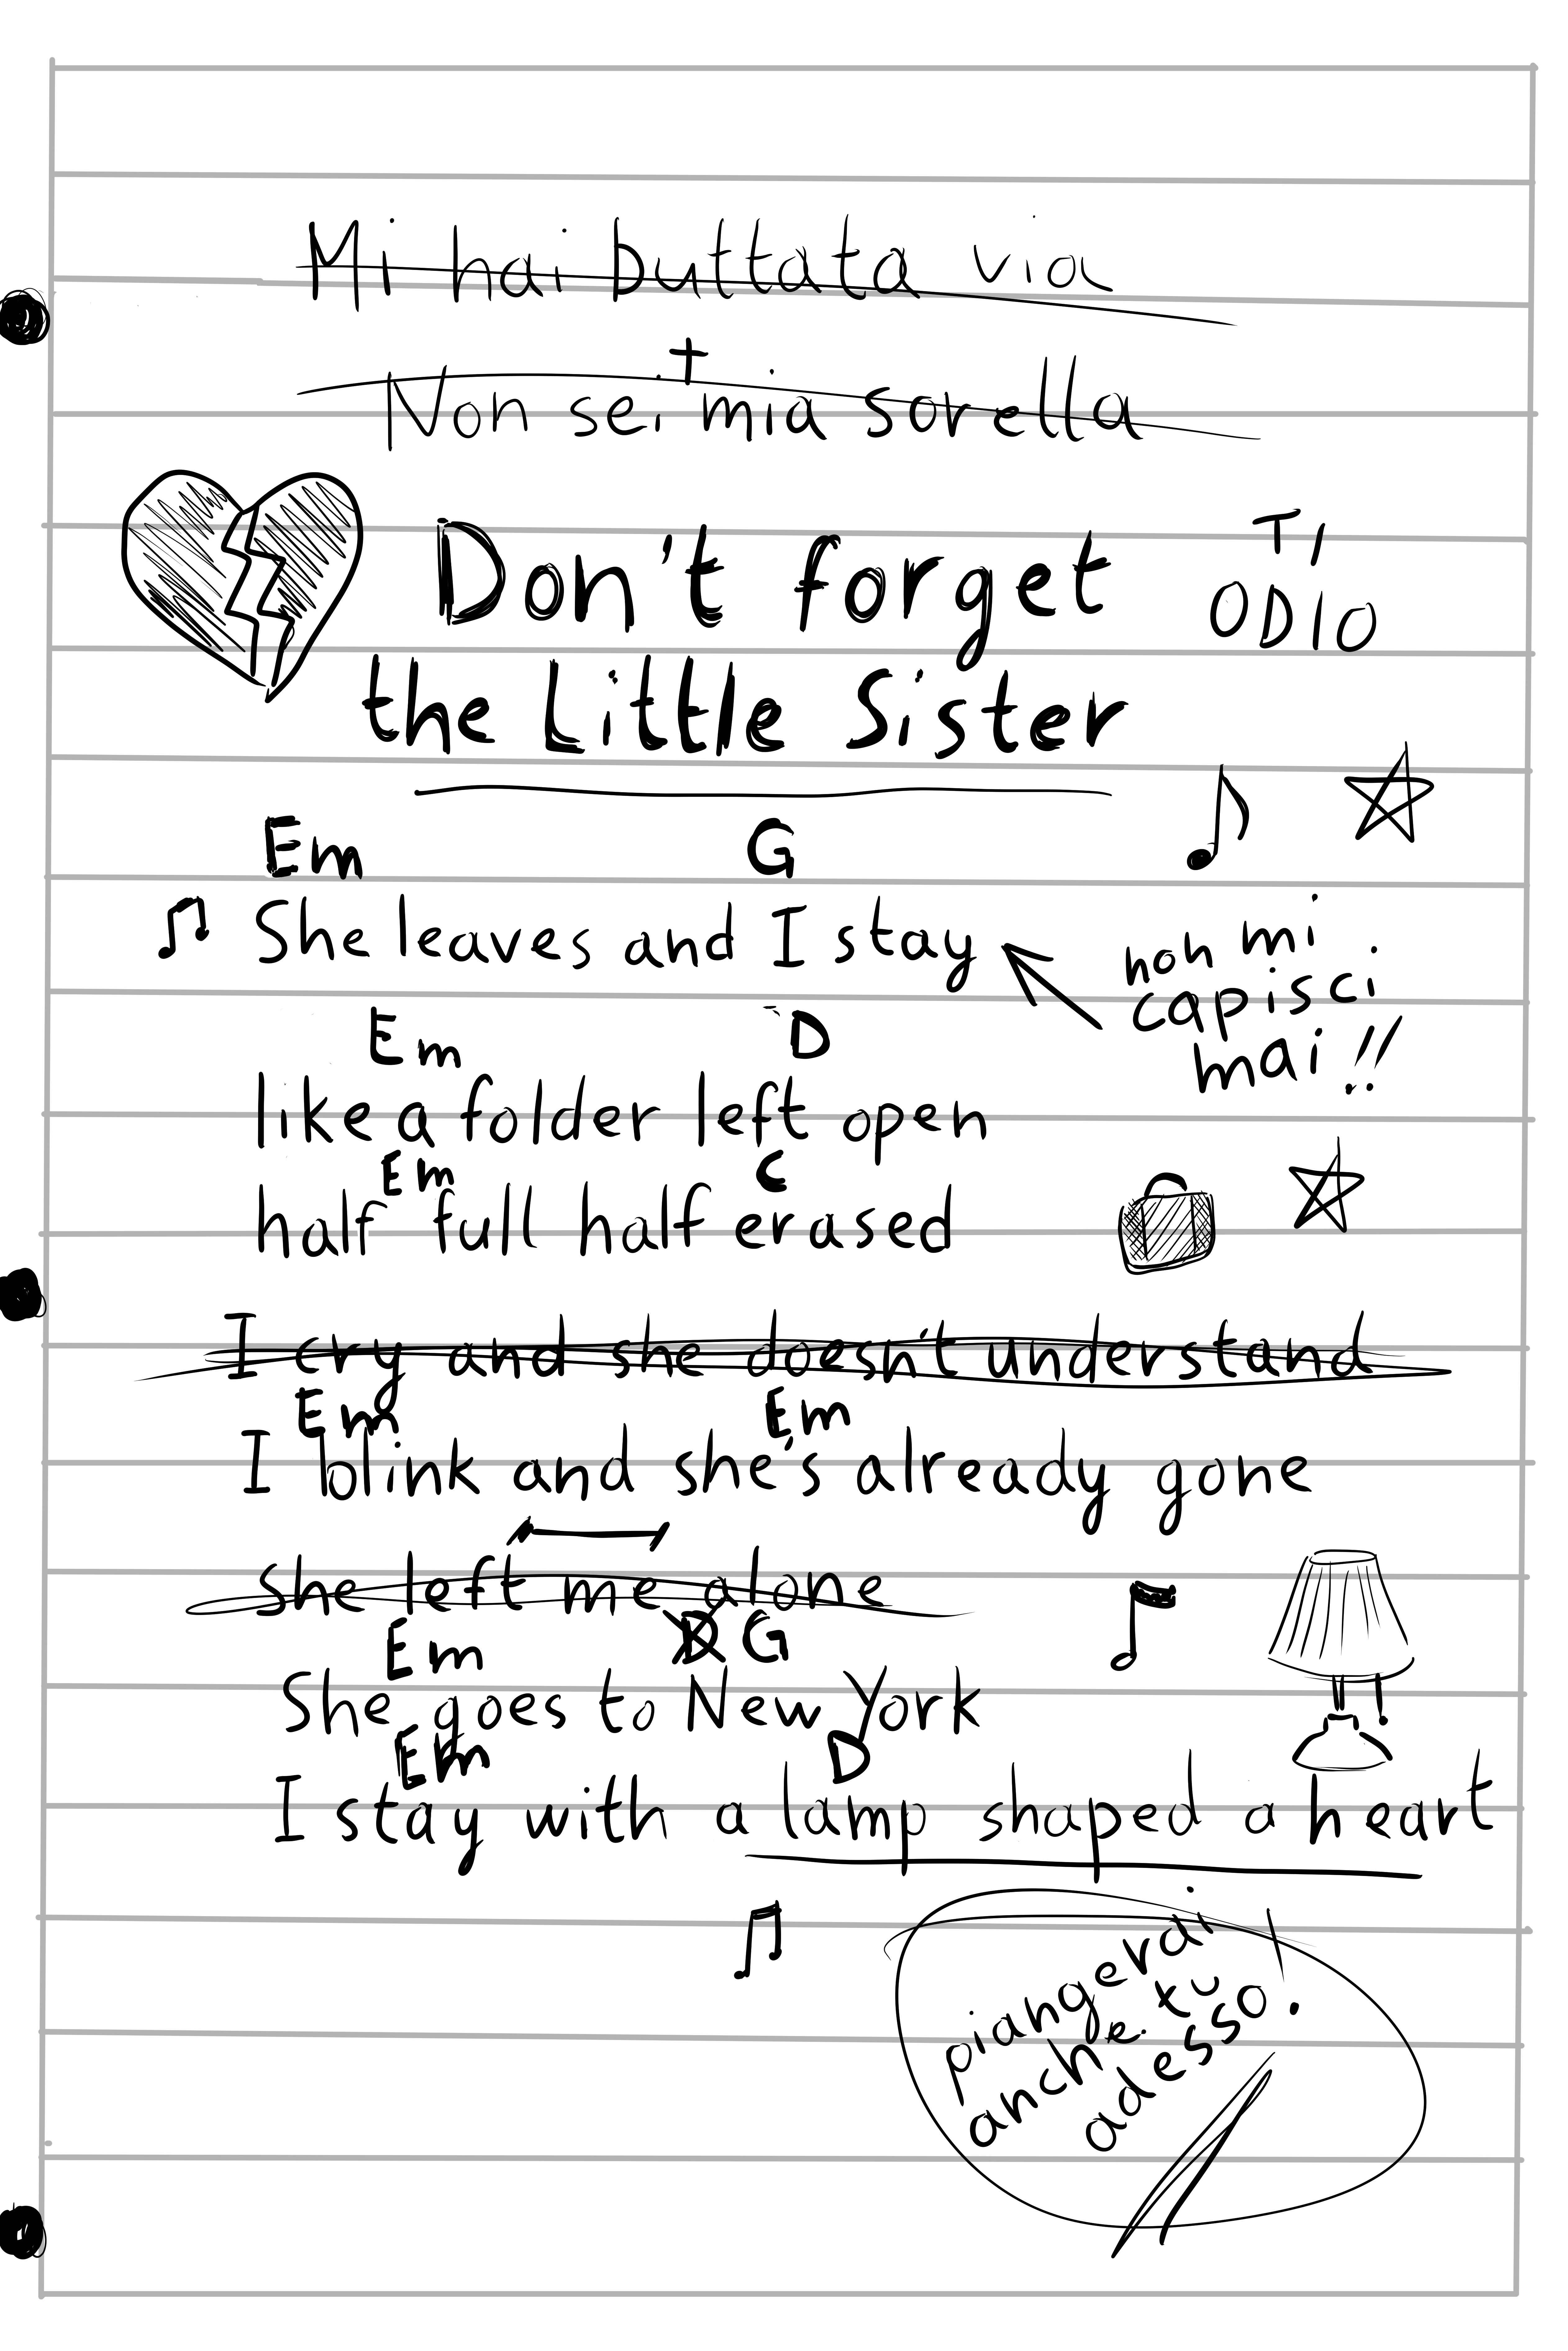
\includegraphics[width=.70\linewidth]{diario alice senza sfondo.png}
  %\caption*{\footnotesize Le parole della canzone sul quaderno di Alice, con accordi per la chitarra.}
\end{figure}

Questa è Alice, quasi grande ma ancora adolescente; a vederla nel suo vestitino skater non sembra capace di parole così taglienti.

\begin{figure}[H]
  \centering
  \includegraphics[width=.70\linewidth]{alice senza sfondo.png}
  %\caption*{\footnotesize Alice piange mentre suona la sua canzone.}
\end{figure}

\pagenumbering{arabic}
\setcounter{page}{1}
\pagestyle{plain}



% --- 17 capitoli ---
\chapter{Vendetta in SOL maggiore}




Laura, seduta sulla poltroncina \textit{for friends}, aiuta l’amica a sbrigare un po’ della corrispondenza mentre lei è impegnata in altre faccende che le stanno più a cuore.

\par\medskip
\begin{center}
  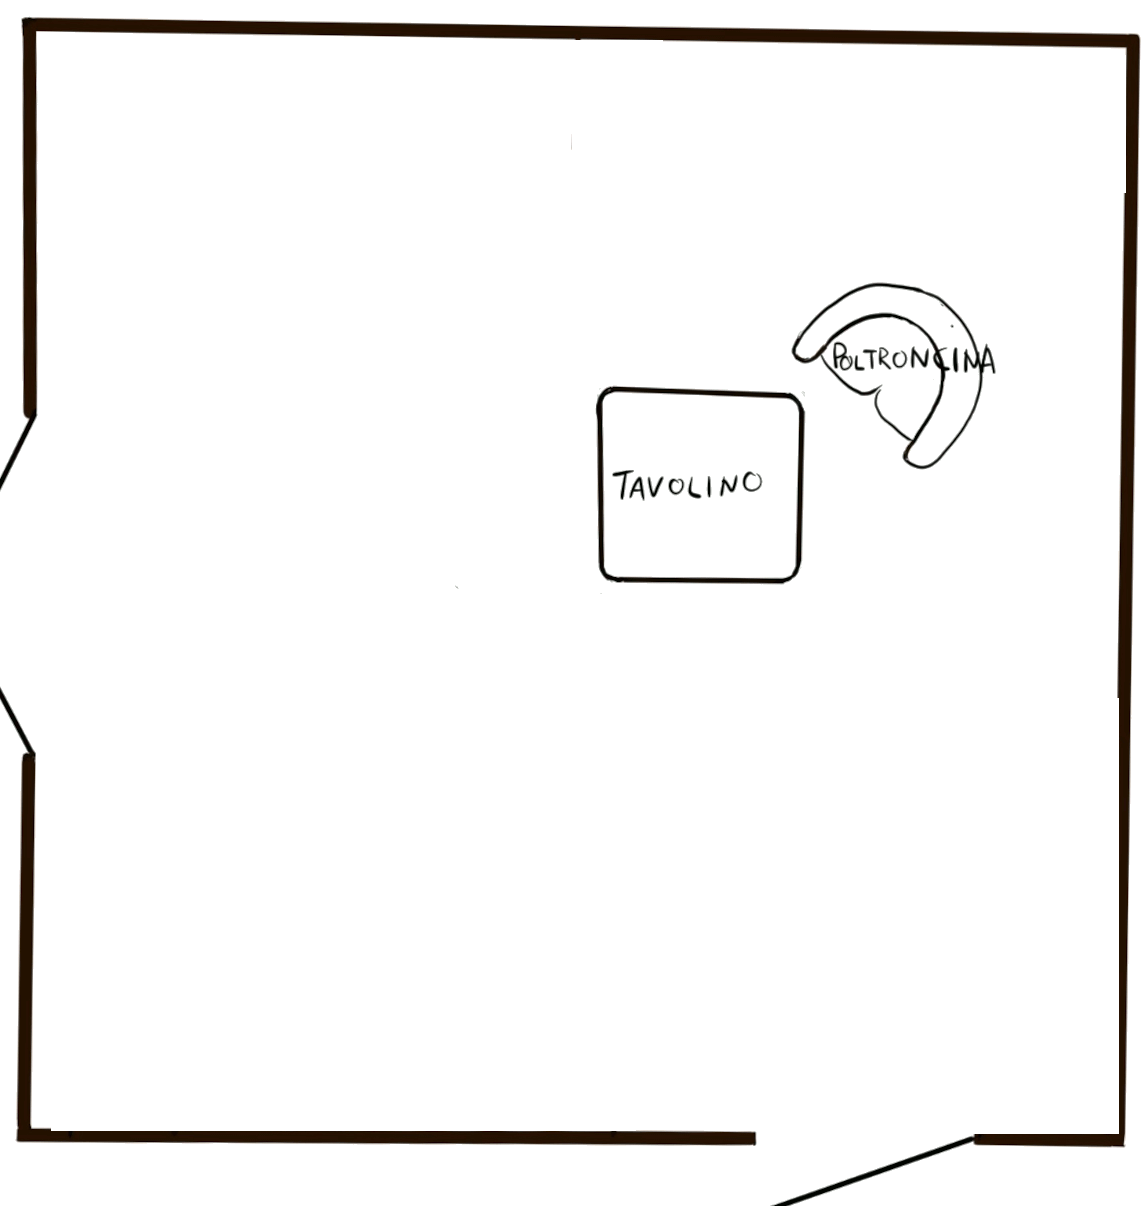
\includegraphics[width=.75\linewidth]{image1.png}
\end{center}

Una lettera è un messaggio scritto di pugno e consegnato nella buchetta di casa per mezzo di un servizio postale.
Per molte persone ha un significato simbolico: indica l’appartenenza al gruppo di chi non ha dimenticato l’origine terrestre degli esseri umani.
In molti si sono convinti che la carta non sia il male del mondo ed esprimono con le parole il loro dolore per il pianeta che soffre, scrivendole con la matita, sulla carta.
Una matita fatta di legno sulla carta di cellulosa.
Parole fatte di albero, spedite a destinatari incaricati di sorreggere il peso dell’angoscia collettiva.

\begin{verse}\itshape
«Cara Caterina,\\
ti scrivo con le mani sporche di terra e il cuore in fiamme.\\
Ogni giorno mi sveglio con l’ansia che il cielo sia un po’ più basso,\\
che il vento porti con sé un alto grido soffocato di una specie che non c’è più.\\
Eppure continuo a lottare, perché se ci sei tu,\\
tu che hai il coraggio che io non ho…»
\end{verse}

«Vuoi che continui, Cate? Non mi sembra aggiunga nulla di nuovo alla discussione…»\\
«Ma sì dai, mi sembra così angosciata, poverina…»
\par\medskip
Caterina è a pochi decimetri da Laura, davanti all’armadio
\par\medskip
\begin{center}
  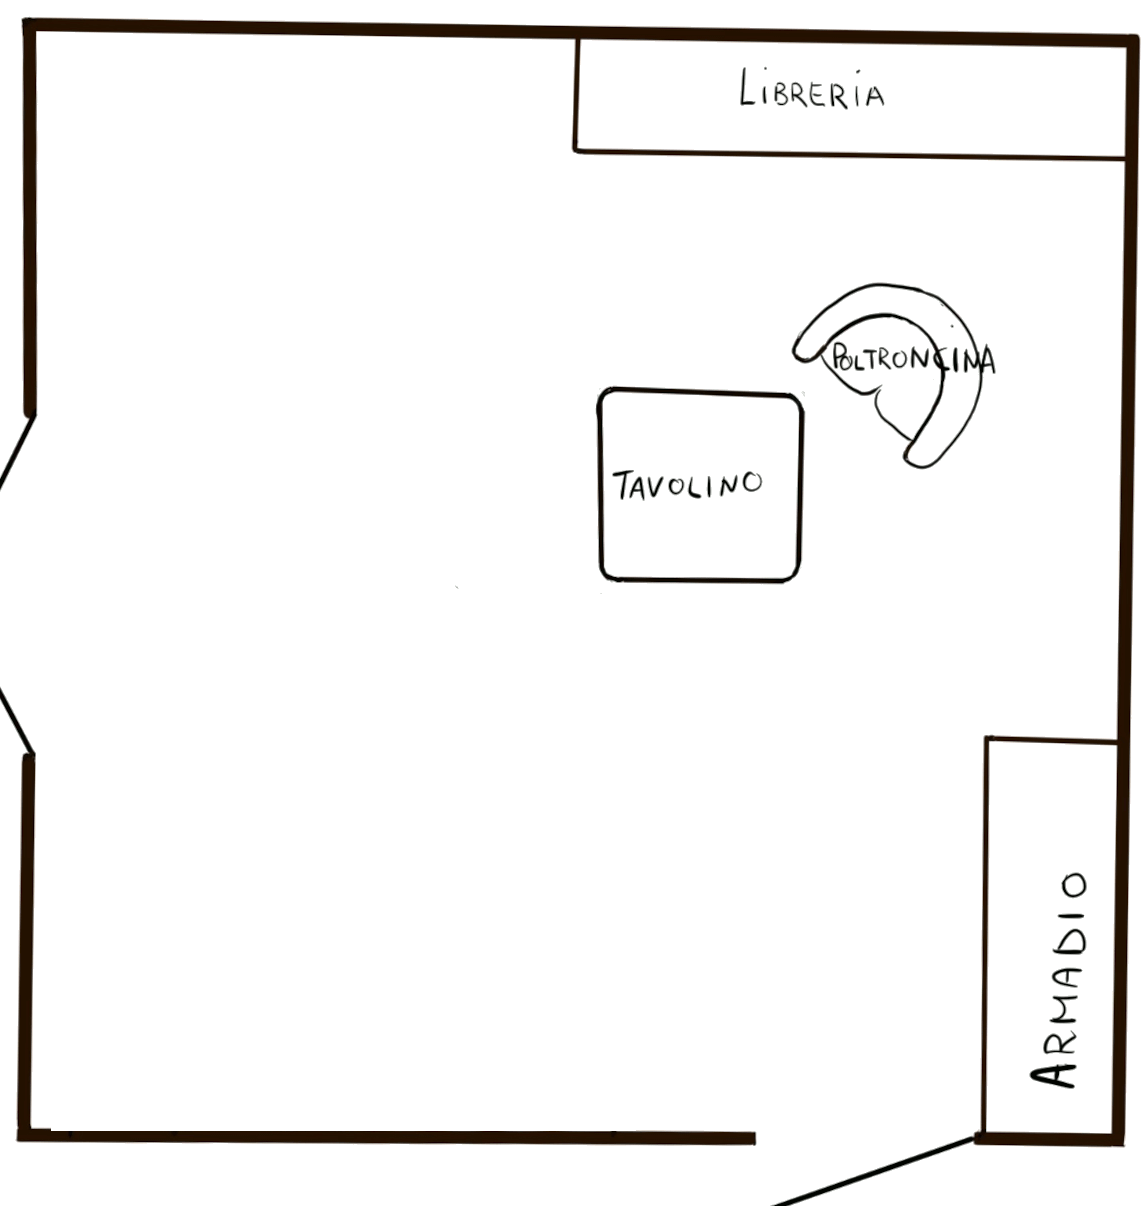
\includegraphics[width=.75\linewidth]{image3.png}
\end{center}

che sceglie i vestiti da mettere in valigia.

Laura riprende a leggere ma il settanta per cento delle parole sfugge alla sua attenzione focalizzata sui movimenti mimetici di Alice che seduta sul letto sul letto di fronte a lei armeggia con un vecchio portatile ostentando disinvoltura.\\

Caterina è su di giri, ma esausta. Tra biglietti introvabili, alberghi al completo e impegni incastrati all’ultimo, è stato un viaggio difficile da organizzare.

Mancano trentasei ore al volo che la condurrà negli Stati Uniti ed è quasi tutto a posto, ma  non sa ancora che sua sorella le sta cucinando una bella vendetta da gustare calda anziché fredda.

Caterina  va a New York lasciando Alice a casa con suo padre e sua madre: \textit{proprio ora che potremmo passare una settimana insieme} rimugina Alice continuando a scrivere sulla tasiera.  
Certo, Alice comprende che il lavoro è importante e se si trattasse  solo di lavoro, non le brucerebbe così tanto.

Ma il problema è un altro: \textit{lei ci va per Mark}.  
Figurati, se non ci fosse stati lui, avrebbe sicuramente preferito passare l’estate con lei.  
In fondo, di corsi di aggiornamento ce ne sono tanti nel mondo.  
\textit{Lei ci va per Mark.}

\par\medskip
Così, tranquilla, con il PC in mano e le gambe incrociate sul letto, mostra uno sguardo innocente, perfettamente a suo agio nell’ambiente. Intorno a lei, però, non c’è la sua stanza.  
È la camera di Caterina: ordinata, spaziosa, un piccolo ecosistema.

Dalla camera di una ragazza si può capire molto di lei.

\par\medskip
\begin{center}
  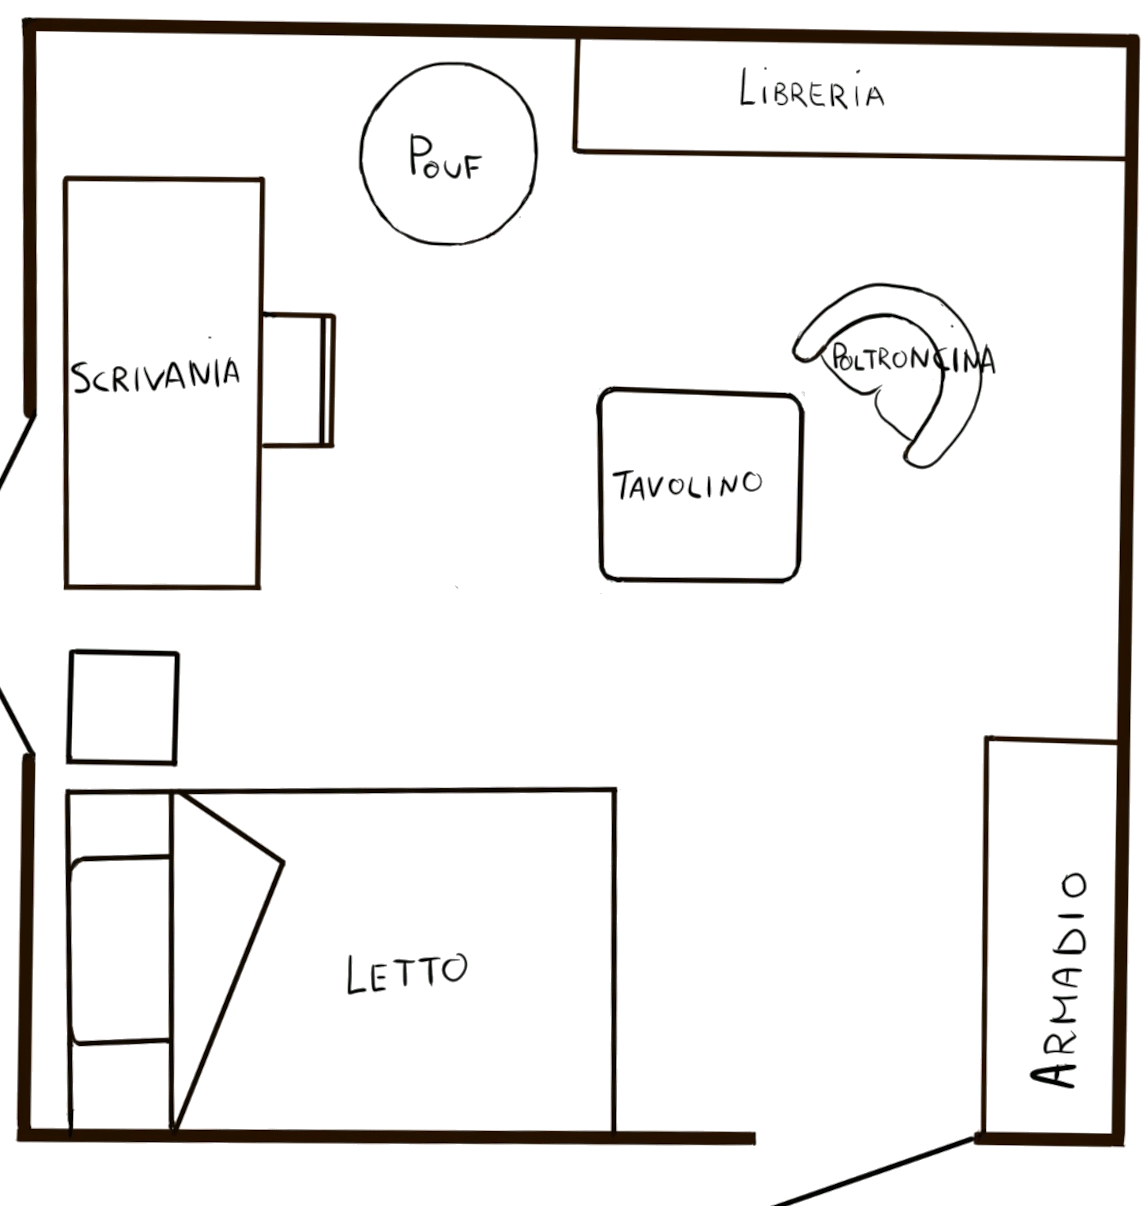
\includegraphics[width=.75\linewidth]{image2.png}
\end{center}

L'ampio spazio al centro racconta del suo cuore e della libertà di cui ha bisogno. I mobili accostati alle pareti testimoniano, involontari, il suo bisogno di organizzazione e sicurezza, fisica e affettiva, quella che Alice continua a sfidare creando una tensione forte e percepibile, ma senza spiegarne la ragione.
Laura però vuole capire,  si avvicina per sbirciare cosa stia facendo, ma Alice, con una piccola rotazione, si sottrae al suo sguardo.

«Scusami, sai!» la rimprovera dell'indiscrezione.  
Poi incolla il testo nella sezione \textit{Lyrics}:
\pagebreak
\par\medskip
\textbf{Lyrics}
\begin{quote}\itshape
She leaves and I stay\\
like a folder left open\\
half full, half erased\\
I blink, and she’s already gone
\end{quote}

«Qui capirai quanto ci sono rimasta male…»

\par\medskip
\textbf{Style Description}
\begin{quote}\itshape
Bilingual emotional synth-pop with ambient textures, cinematic flow, and AI female vocals.\\
Slow build. Glitchy, dreamlike, bittersweet. Like diary pages sung in code.
\end{quote}

«Lasciala perdere, è arrabbiata con me.»

«Non sono arrabbiata, solo che voglio finire una cosa.»

«Ha ragione, sono io che sono troppo curiosa.  
Però si è fatto un po’ tardi, è ora che vado a prendere Valentina.»

«No, aspetta solo un attimo, ti prego.»

«Ora la scarico, colleghiamo le casse e voilà!»

\par\medskip
Le note di pianoforte sintetico arpeggiano velocemente una nenia in Sol maggiore.  
Poi, con un respiro sussurrato, inizia il primo verso:

\par\medskip
\textbf{Verse 1}
\begin{quote}\itshape
She leaves and I stay\\
like a folder left open\\
half full, half erased\\
I blink, and she’s already gone
\end{quote}

Questa è la scena prima della crisi…

\par\medskip
\begin{center}
  \includegraphics[width=.75\linewidth]{ccsf.png}
\end{center}

\textbf{Verse 2}
\begin{quote}\itshape
She goes to New York\\
I stay with a lamp shaped like a heart\\
plastic love, three settings\\
warm, cold, ambient — mine is blinking
\end{quote}

«E qui voglio vederti piangere!»

\begin{quote}\itshape
I'm not angry, I'm just here
\end{quote}
Caterina continua ad ordinare le cose da mettere in valigia, mentre una lacrima le riga il viso. Laura la vede scendere piano fino alla guancia, lì Caterina la ferma, pulendosi con i polpastrelli. «Certo che le semplifichi proprio la partenza, tu.» Le parole di Laura sciolgono Caterina che appoggia l’asciugacapelli e si avvicina alla sorella per abbracciarla.

«Non ci provare!» le urla Alice.

Caterina non reagisce. È abituata.  
Alice si libera le ginocchia dal PC e lo poggia sul letto.

«Io esco, mangio qualcosa con le mie amiche.»

Caterina si asciuga gli occhi. Ormai è inutile simulare.

«Va bene, ma torna a casa per le dieci. È l’ultima sera che passiamo insieme.»\\
Laura si alza e si sistema i vestiti:
«Devo andare anch’io, Cate.»
\\
«Va bene Laura, grazie di essere venuta.»
\\
«Ciao Cate. Ciao Alice.»
\\
Prima di chiudere la porta, Laura ha un attimo di esitazione.  
C’era ancora una cosa, anzi, era il motivo principale per cui aveva raggiunto Caterina.

«Ma non sai ancora nulla del visto?»\\

«Non preoccuparti, Laura. Vedrai che non ci saranno problemi.  
In ogni caso, se ci fossero difficoltà ti chiamo.»

Saluta l’amica con un bacio e corre a prendere Vale.  
Per fortuna manca ancora qualche anno alla sua adolescenza.

% chapters/chapter02.tex
\chapter{Si sta facendo sera}

Caterina \`e impegnata nei preparativi per il suo volo transoceanico con cui spargerà dieci quintali di CO$_2$ nell'atmosfera. Giovanni attende con Ipparchia un po' di cibo recuperato dalla distribuzione ordinaria. La sua impronta di carbonio \`e bassa per necessità, non per scelta. Vive nell'ex convitto  "San Giorgio", senza i comfort di un'abitazione urbanizzata, e produrre pi\`u CO$_2$ di quella che espira \`e quasi impossibile.

\par\medskip
Ipparchia \`e seduta sotto una quercia vicino all’uscita sul retro, la \emph{dumpster zone}. Da un momento all’altro i commessi usciranno per le pulizie e quello sarà il segnale. Giovanni aspetta con calma, pronto a contrattare qualche prodotto in scadenza.\\

La porta si apre: Ipparchia capta il segnale e si fa avanti. Giovanni attende, non si muove subito: aspetta un cenno di invito. Ripensa alle parole di sua madre, un mantra: \textit{La prima regola  \`e la buona educazione}. Quando la ragazza  lo chiama, Giovanni ricambia con un sorriso. Lei rientra per uscire di nuovo con un cartone che non deve essere troppo pesante a giudicare dalla nonchalance con cui lo destreggia.

\begin{center}
  
\includegraphics[width=.9\linewidth]{media/dumper_zone.png}
\end{center}



\par\medskip
Lo appoggia al pianerottolo delle scale di servizio. Ipparchia tira Giovanni e i due si avviano verso di lei, in equilibrio tra zelo e prudenza. Lei li aspetta  e mentre si avvicinano
 accende una sigaretta. \`E tanto giovane da credersi immortale.

\par\medskip
«Ciao Giò, ciao bella!»

\par\medskip
Ipparchia accetta la carezza e ricambia il saluto ricevuto.

\par\medskip
«Ti fa male fumare», le dice sorridendo.

Lei lo guarda per un istante. Tira ancora qualche boccata poi la spegne.

\par\medskip
«Torno dentro!»\\
«Ti ho rovinato la sigaretta.»\\
«Macché, devo riprendere il turno.» Apre il portone. «A presto, vi aspetto.»\\
«Grazie, prendo il pacco!»

\par\medskip
Adesso deve portare il pacco al convitto. La strada non \`e lunga, ma Giovanni deve ricordarla a memoria. Nella mente ha catalogato strade, stradelli, edifici, alberi e piante, organizzati in strati come nelle mappe  governative digitali.
\par\medskip
La vegetazione per\`o cresce rapidamente, l’edera inghiotte metri di strada ogni mese, i rami delle siepi invadono i marciapiedi, e la topografia ufficiale resta sempre un passo indietro rispetto al mondo vivo.

Ma tra i neuroni naturali di Giovanni si annidano connessioni che lo strato cognitivo del tecnocene non ha ancora registrato.

Lui ha esplorato siepi campestri, corridoi ecologici, fasce ripariali e margini di bosco. Quei luoghi sono l\`i, dentro di lui, con i loro merli, le capinere, i ricci, le arvicole, i fagiani, i ramarri e gli impollinatori. I nidi di quegli insetti non sono presenti nei database, ma il \textit{Prunus cerasifera} fruttifica anche grazie a loro, e Giovanni ne mangia chili ogni estate.

\par\medskip
Questa \`e la mappa che Giovanni ha nel cervello: odori, superfici, distanze misurate a passi e colpi di bastone.
Una  mappa che va aggiornata di continuo: dove la memoria vacilla, ci sono il fiuto e gli occhi di Ipparchia.


\begin{center}
  \includegraphics[width=.82\linewidth]{"media/mappa di odori.png"}
\end{center}


\par\medskip

\par\medskip
Ipparchia \`e al suo fianco da quando Giovanni \`e diventato un senza fissa dimora. Anche lei vagava sola e il loro incontro sarebbe stato degno di una nota nei rotocalchi se qualche giornalista lo avesse testimoniato. Questa \`e la vita di strada, capita di tutto, ma nessuno se ne cura. Ipparchia non lo tradirebbe mai.
\par\medskip

Un fagiano, disturbato dalla loro presenza, esce da una siepe e gli taglia la strada. Giovanni sente solo un fruscio veloce dell’erba, Ipparchia si lancia dietro al fagiano e i due scompaiono nel corridoio ecologico.
\par\medskip
Giovanni \`e solo, con uno scatolone in mano e la sua compagna da ritrovare prima che corra in un luogo fuori dalle sue mappe.

\par\medskip
Il silenzio si stende, pesante, tra le erbacce. Giovanni ascolta il suo stesso respiro, poi si rimette in cammino.





\chapter{Il ricorso}
Ed eccoci a casa di Laura. \'E arrivata in tempo a predere la sorella e ora Valentina sta finalmente sul tappeto  con le sue matite e i suoi pennarelli. Laura invece  è al lavello che prepara la cena con  un orecchio  teso cerca di decifrare i  borbottii e i sussurri che riesce a captare. Mezze frasi, accenni  a mondi fantastici. Continenti a forma di frutta, paesi costellati da piccoli laghetti, villaggi fatti solo da alberi,  terre aride e disastrate dove vivono popolazioni tornate alla barbarie. Tutto in un foglio di una cinquantina di centimetri per quaranta.

Poi, quando l'odore delle zucchine  raggiunge il naso della piccola,  un pensiero più concreto sospende tempraneamente la sua attività, lasciando la priorità alla contingenza:
«Cosa prepari per cena?» domanda.\\
«Tu cosa avresti voglia di mangiare?»

\par\medskip
\begin{center}
  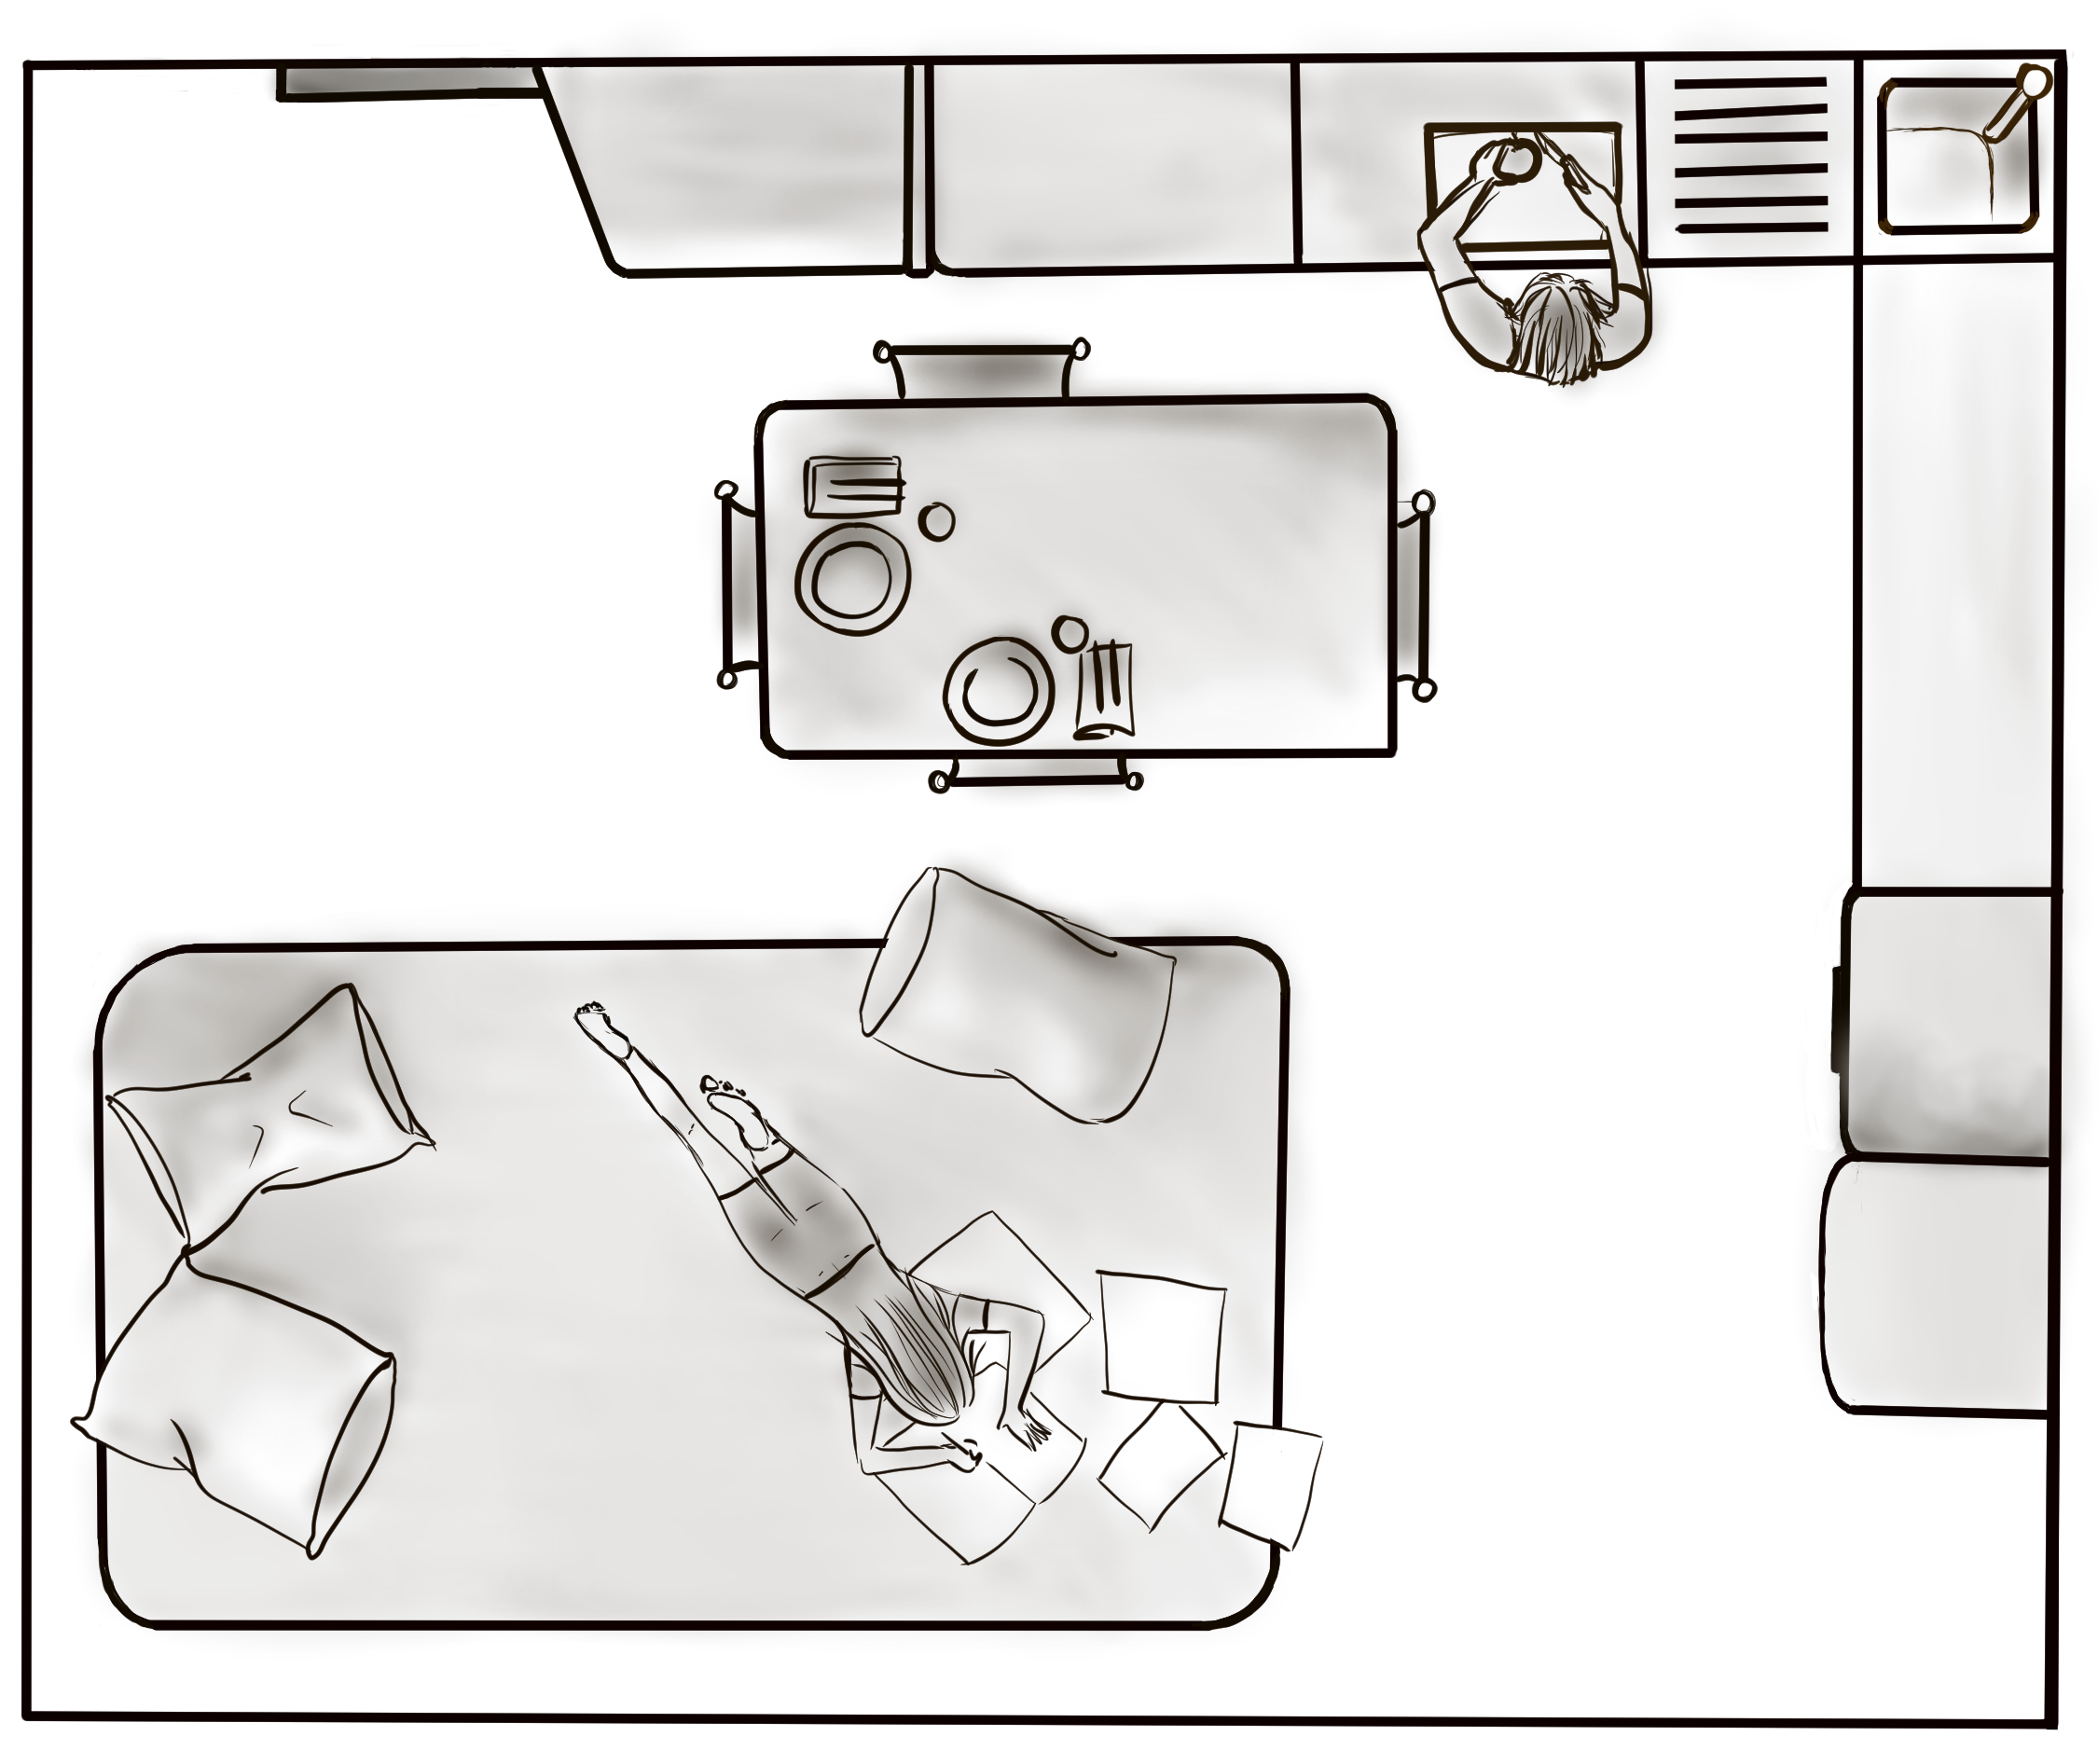
\includegraphics[width=.7\linewidth]{soggiorno_tiny.png}%
\end{center}

«I bastoncini fritti! Prepari i bastoncini fritti?»\\
«Infatti.»\\
«Davvero ci sono i bastoncini?»\\
«No, c’è il riso integrale con le verdure.»\\
«Perché sempre le verdure?»\\
«Perché ce ne abbiamo nell’orto, sono buone, fanno bene e non escono dal tubo.»\\
«Blaa...il pastone...» Valentina fa una smorfia. «Ma io ho voglia di bastoncini. Quando li mangiamo?»\\

«Venerdì. A fine settimana acquisterò del cibo. Dobbiamo mangiare tutti i principi nutritivi.»

Da sotto il tavolo Rocky si alza e si avvicina alla porta. Laura lo segue con lo sguardo «Cosa hai visto?»\\
Rocky abbaia. Laura si ferma di tagliare: «Guarda, arriva Caterina. Non farle vedere che fai i capricci per la cena.»\\
«Non è vero che faccio i capricci.» Intanto l'amica è arrivata alla porta, bussa e fa scorrere l'anta di vetro, ma si arresta sull'uscio.\\
«Ciao Caterina, vieni dentro» la invita Valentina.\\

«Ma guarda che confusione!» la voce di Caterina ha qualche accento di rimprovero. «Penne, pennarelli» continua,  «lapis, fogli da disegno mi sbarrano la strada e un Cerbero feroce non mi lascia passare! Come posso entrare, signorina?»\\
«Salta!» le risponde, «E tu seduto, Rocky!».



\par\medskip
\begin{center}
  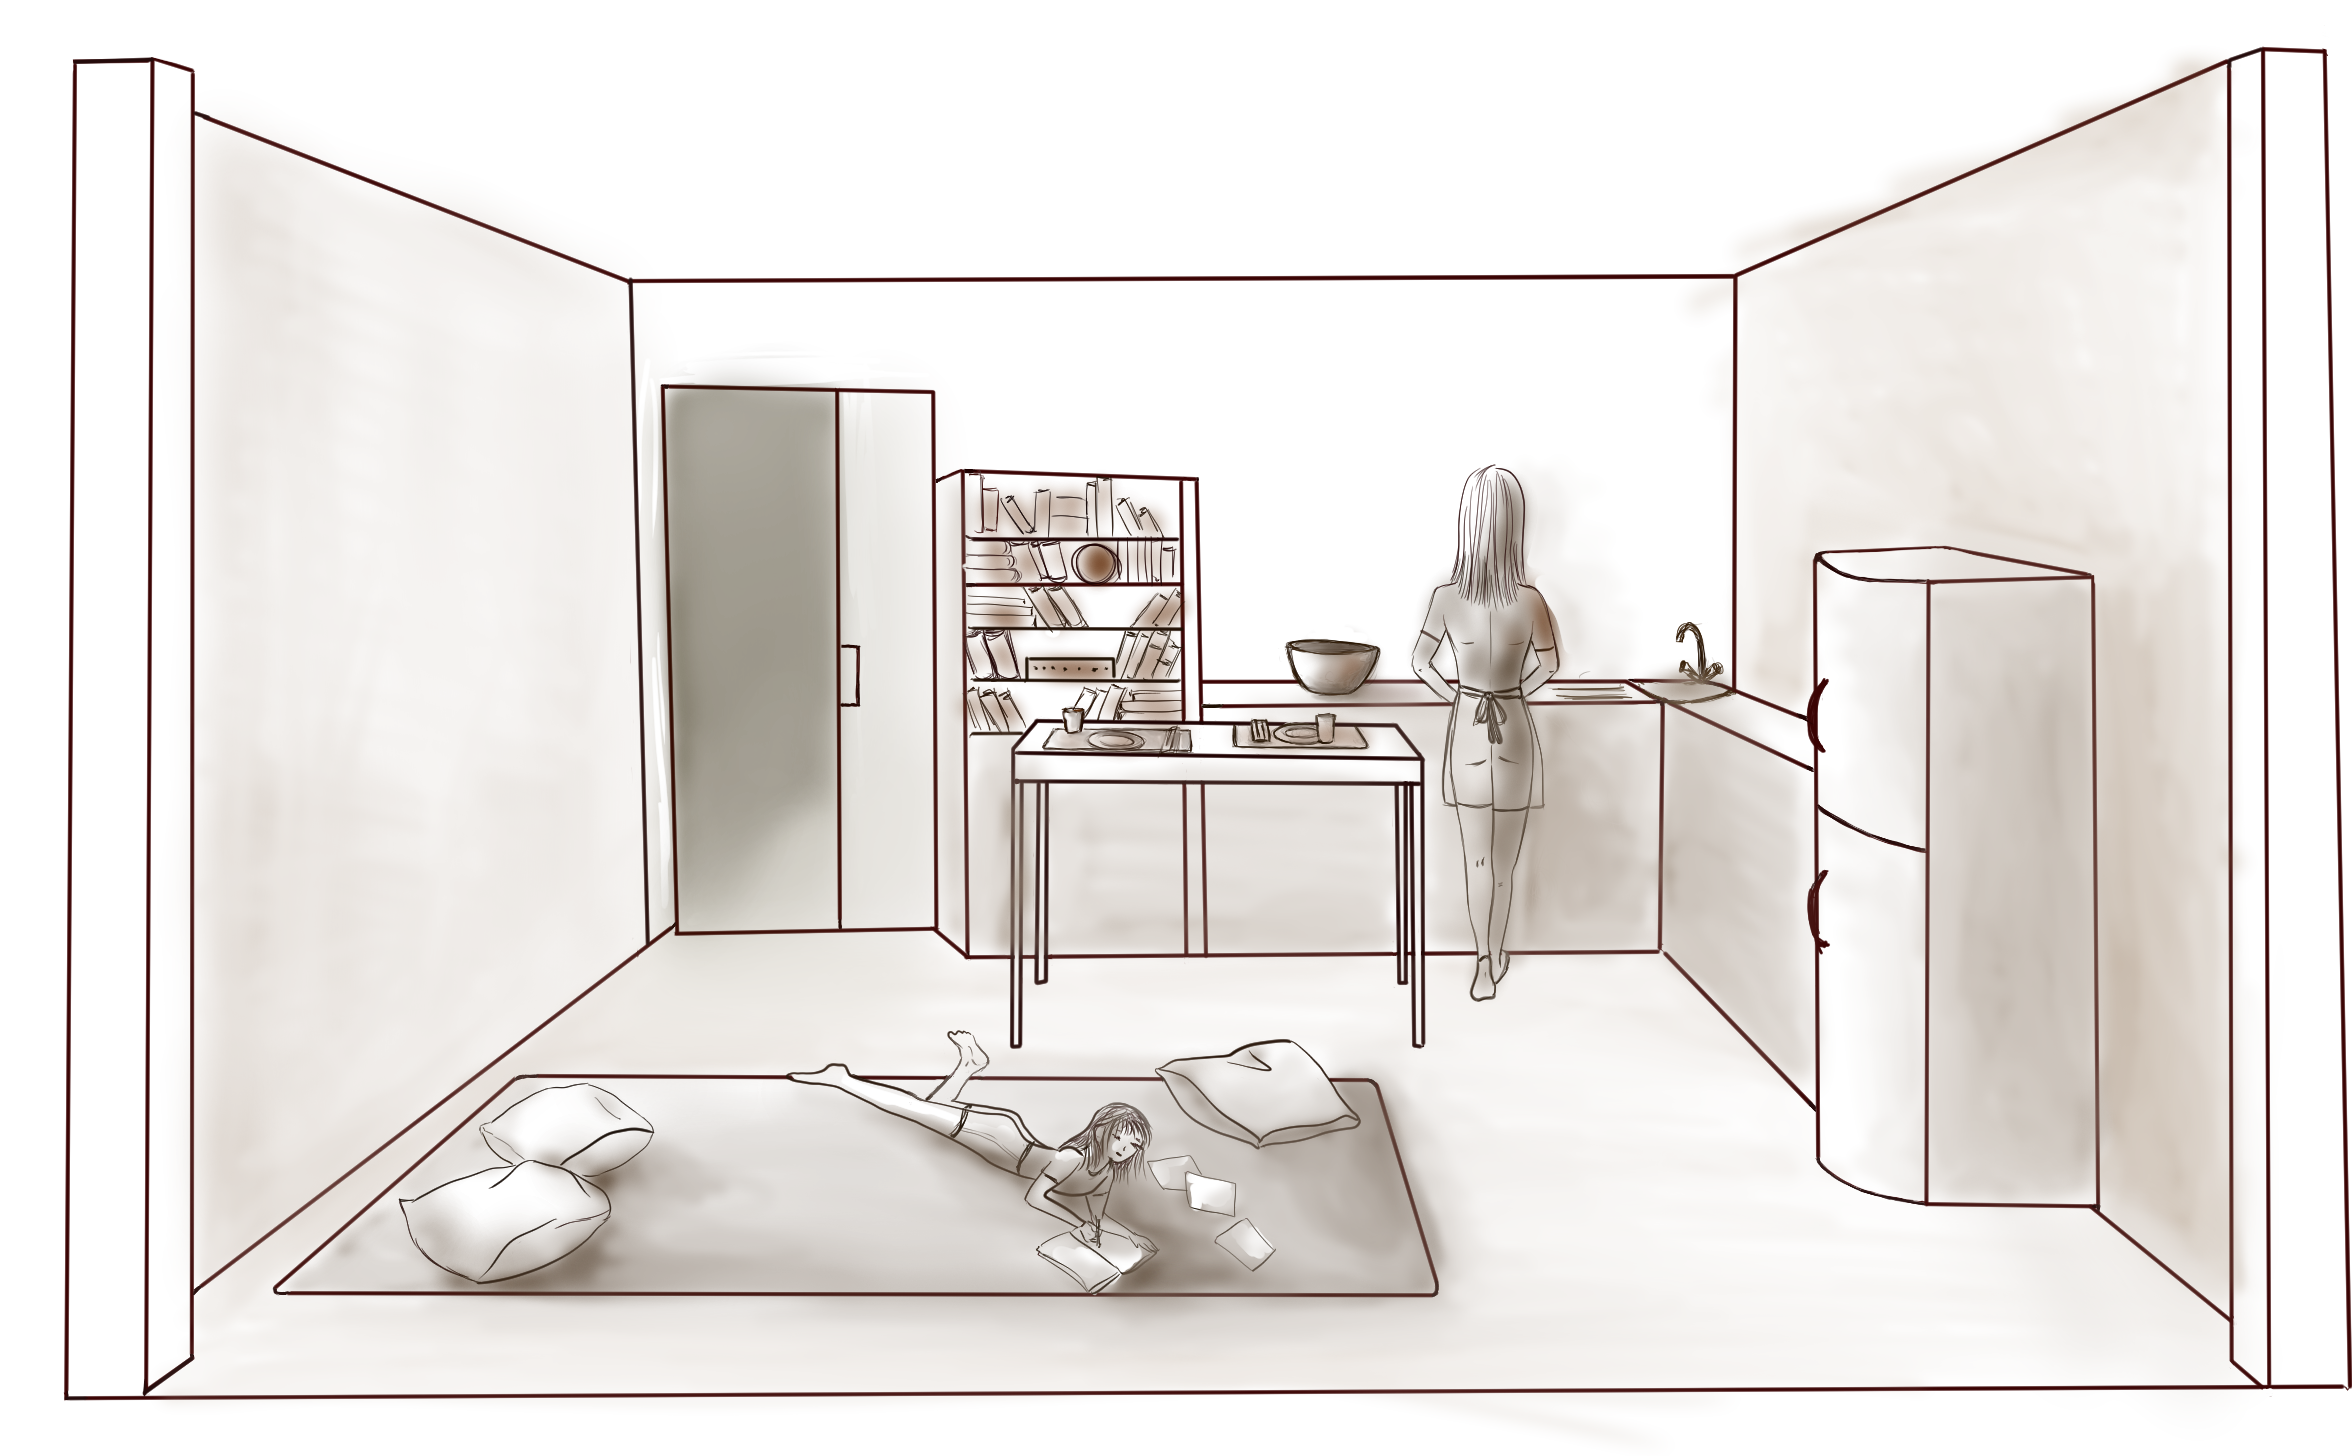
\includegraphics[width=1\linewidth]{soggiorno_prospettiva.png}%
\end{center}
Si alza dal tappeto, prende Caterina per mano, la trascina dentro con un piccolo salto sopra la distesa mentre Rocky torna a sdraiarsi sotto il tavolo.
Valentina lo guarda: «Non ha tre teste...» protesta.\\
Il grande foglio che hanno appena saltato attira l'attenzione dell'amica che vi si inginocchia vicino.

«Cosa disegni? \'E un compito?»\\
Valentina scuote veloce la testa da una parte all'altra come una campana: «Anche, ma non solo. Stavo disegnando una cosa. Vedi questo mare?»\\
Caterina si avvicina: «Si, le vedo» conferma.\\
«Divide due regni. Da una parte ci stanno i buoni»  ed indica il disegno di due uomini visibilmente forti, «dall'altra loro, che sono i cattivi.» Questa volta sposta il dito su tre figure maschili con tratti feroci.


«Fanno proprio paura» conferma Caterina cercando Laura con lo sguardo. Lei però è ancora intenta alla preparazione della cena, ma colta una vena di preoccupazione nella voce dell'amica la tranquillizza: «Fanno paura anche a me,» le conferma, «ma ha trovato la libreria manga dei miei e adesso non la ferma più nessuno.» \\
Caterina non risponde, Valentina l'ha preso un braccio tirandosela vicina. «Ti fanno paura? Davvero?»\\
«Il tuo disegno è bello, ma loro sono davvero brutti. Quindi?» Le chiede, «In che regno sarebbero questi brutti mostri?»\\
Valentina appoggia il foglio, «Loro abitano nella terra degli Shura.»\\
«E dove si trova?» le chiede.\\
Lo riprende in mano  e indica la regione dove abitano gli eroi buoni: «Se questo è il giappone, questa cosa sarà mai?»\\
Le orecchie di Laura si tendono verso la sorella «Non fare la maestrina con Caterina.» Valentina la ignora e continua: «Dai, che paese si trova a sinistra del Giappone?»\\
«Allora... abbiamo detto che questo è il Giappone? Direi che questa dovrebbe essere» attende un attimio, «dovrebbe essere la Corea» esclama, sicura della correttezza della risposta, ma la delusione non tarda ad arrivare.\\
«Hai studiato geografia da piccola? Lì c'è la Cina» e ciò detto indica con il dito la vicinanza tra le due terre.
«Hai ragione Vale, la Corea è un po' più in là.»
Caterina si inginocchia, pronta ad ascoltare la storia di quei luoghi che sicuramente non è ancora conclusa. Valentina infatti non sembra proprio aver esaurito gli argomenti:

«Ecco, vedi, qui in Giappone invece sono buoni. Loro studiano sempre le arti marziali, in questa scuola» e indica una casetta.
Caterina  avvicina gli occhi al disegno.

«Sì? E in questa scuola c’è anche un maestro?»\\
«Certo, è il padre dei tre fratelli. Adesso ti spiego bene» e parlando si posiziona veloce un cuscino sotto le ginocchia, ma viene interrotta dalla sorella:
«Vale, forse Caterina doveva dirmi qualcosa. Sentiamo?»\\
Caterina sorride,
«Si, ma lascia prima che mi racconti. È passato tanto tempo da quando Alice  mi mostrava i suoi disegni. Non pensavo mi mancasse così tanto.»
\\
«Anche Alice fa i disegni? La prossima volta voglio vederli.»\\

«Li faceva da piccola tesoro, adesso mi scrive le canzoni.»
\\
«Che bello, allora le voglio ascoltare!»\\

Caterina le sorride e appoggia il disegno sul tavolo seguita dallo sguardo corruciato di Valentina che prontamente lo va a riprendere.\\

«\'E andata male» il tono è quello riservato a Laura, non parla più con Valentina. «Mi hanno negato il visto. Ho tempo fino alle ventiquattro per fare ricorso.»\\

Laura appoggia il coltello sul tagliere e guarda verso l’amica:

«Quando l’hai saputo?»\\
«Due ore fa eri a casa mia e non lo sapevo ancora... quindi?»\\
«Hai ragione, Cate, scusami.»\\
«No, scusami tu. Sono stata acida. È che sono disperata.»\\
«Ma hai già sentito Mark?»\\
«Sì, è stato lui a dirmi della possibilità di fare ricorso.»\\
«Oh, Laura, come facciamo?»

Laura si avvicina all'amica e la prende delicatamente per le braccia:

«Cate, ne abbiamo passate di peggio. Se il tempo stringe, vediamo prima il ricorso, poi mangiamo.»\\

Valentina le ascolta distrattamente:
«Non ceniamo?» chiede, ma non ricevendo risposta dimentica la fame come solo i bambini sanno fare e ritorna a colorare.\\

In camera da letto ha un tavolino basso, lo prende insieme al suo computer  portatile e lo appoggia tra il tappeto e il frigo: «Mi fai un po' di posto Vale?»\\
«Cosa fate con il computer? Posso vedere?»\\
«Cose da grandi» le risponde Laura. Valentina non replica, si siede a fianco di Caterina. Laura collega il dispositivo ad una rete dati separata da quella domestica:

«Vediamo, quindi Mark lavora per la SAGA-M, giusto?» La connessione è stabilita e Laura accede a un servizio di informazioni basato su un protocollo dati testuale, un po' datato ma ancora in uso. È alla ricerca della SAGA-M. Caterina allunga il collo verso lo schermo:
«Sì, perché? Cosa stai cercando?»\\

«Voglio capire cosa le interessa e cosa invece la preoccupa...»\\
«Laura ti prego sii più chiara... mi stai facendo salire l'ansia, non guardiamo la procedura per il ricorso?»\\
Laura chiude alcune schede poi avvia un monitor a caratteri, uno sguardo rapido all'amica: «Scusami... hai ragione. Adesso... vedi, tu non sei mai stata negli Stati Uniti, giusto?»\\
«No, è...» si ferma, «sarebbe la prima volta.» Risponde Caterina. Valentina si sdraia sul tappeto, prende un pennarello e si disegna un cuore sulla mano.\\
«Quindi non hai commesso nulla là che possa precludere il tuo visto... Però è possibile che un'informazione su di te attivi un qualche flag di allarme...»\\
«Ma la privacy?»\\
«...La privacy riguarda la tua sfera privata, non quello che fai in pubblico...»\\
«Non capisco bene il ragionamento Laura...» L'attenzione per un attimo è attratta da Valentina, si è tolta le calze e si sta colorando anche i piedi, Caterina non vorrebbe, ma le scappa da ridere. Si riprende, è preoccupata per il suo viaggio: «Ti servono informazioni per fare ricorso?»\\
«La possibilità di fare ricorso è più apparenza che sostanza, nella pratica è un algoritmo che decide e se non capiamo davvero cosa abbia scatenato il rifiuto...»
Laura marca alcune schede dati per l'elaborazione, «ecco la scheda della compagnia...»\\
\begin{terminalbox}
EU Transparency Register
Entry extract / Interests represented
Reference: EUTR/SAGA-M/ENER/2041-06
Registrant: SAGA-M European Affairs Office

Settore: energia, reti intelligenti,
resilienza urbana.
Policy UE: Green Deal, AI Act,
infrastrutture energetiche.
Comunicazione: autonomia abitativa, mobilita' individuale,
riduzione della dipendenza da nuclei
familiari stabili.

Campagne:
- Single by design
- Non devi nulla a nessuno
- La cura e' un servizio, non un legame
\end{terminalbox}

«Quindi?»\\
Laura inspira profondamente, guarda l'amica:
«Cosa c'entra il "Single by Design" con il green deal?»\\
«Laura mi stai confondendo...»\\

La fissa per un istante, poi abbassa lo sguardo sullo schermo.\\

«Anche io sono confusa, ma se non hai commesso reati e non sei mai stata là, il tuo visto è compromesso dalla tua relazione con Mark e dal suo lavoro... Almeno... Comunque adesso vediamo la procedura per il ricorso, ma poi dobbiamo individuare il nodo che ti ha bloccata, altrimenti il ricorso sarà inutile.»


\chapter{Ipparchia dove sei?}

«Ippa! Ippa! Ipparchia!»\\
La chiama forte, ma lei non torna.

Si siede sul muretto di cinta di un edificio in rovina che non ha mai esplorato, per via di un odore che lo preoccupa: una punta sottile di solvente, insidiosa, che ogni volta gli fa prudere le narici come se volesse raggiungergli il cervello.

Non sa cosa sia stato abbandonato oltre quel muretto e non ha mai cercato di scoprirlo.

Appoggia il cartone sulle ginocchia e aspetta.

Una volta, poco dopo aver perso la vista, gli dissero di attendere il medico: sarebbe arrivato a momenti. Giovanni attese due ore, seduto buono, finché un’infermiera si accorse di lui e lo accompagnò alla visita.

Da allora aveva imparato che “a momenti” può voler dire molte cose. Così, quando deve aspettare, recita i suoi autori preferiti. Spesso Schopenhauer, \textit{L’arte di ottenere ragione}.

«Stratagemma numero uno...»

Lo ripete tutto e, alla fine, sa che è passato circa un minuto. Se fosse stato un matematico avrebbe contato: uno, due, tre. Ma la matematica non era la sua passione.

Arriva allo stratagemma trentotto: è passata un’ora, e Ipparchia non è ancora tornata.

Dietro di lui, un luogo ignoto. Alla sua destra, la strada da cui è arrivato; a sinistra, la strada verso casa. Davanti, una via semi-inesplorata costeggiata da una fascia ecologica, il  margine vivo in cui Ipparchia deve essersi infilata seguendo il fagiano. \'E la direzione più probabile.
Si incammina, continuando a chiamarla.

La strada diventa bianca: l’asfalto finisce e comincia la terra battuta. La fascia ripariale, però, non si interrompe, continua  come un corridoio di odori, il percorso più probabile lungo cui Ipparchia può aver proseguito l’inseguimento.

Quando era scattata dietro al fagiano erano circa le otto di sera; ora è quasi buio. Per Giovanni cambia poco, ma i cani usano anche la vista.

Arriva a un incrocio: la strada bianca curva a destra, la fascia si interrompe, mentre davanti a lui l’asfalto ricomincia.

«Ippa! Dove sei andata?»

Giovanni tiene la destra e si addentra in campagna. Gli alberi continuano a costeggiare la strada, ne conta nove, poi all’improvviso l’asfalto ritorna.

\par\medskip
\begin{center}
  \includegraphics[width=0.9\linewidth]{mappa con casa laura.png}
\end{center}

Attende qualche minuto. Sente passare un veicolo. La strada che ha incontrato taglia quella bianca: deve essere una via principale.

Sta per tornare indietro, quando dall’altra parte arriva un latrato familiare.

«Ippa!»

Attraversa senza esitazione.

«Ippa!»

Le va incontro. Lei rimane ferma. Quando la raggiunge, capisce: il guinzaglio di corda è rimasto incastrato in qualche anfratto. Giovanni lo libera facilmente.

Ipparchia gli lecca la mano.

Ma le lingue sono due.

Un altro cane è accanto a lei.

«C’è un altro cane qui...»

Chiama più volte:

«C’è un cane qui! È di qualcuno questo cane?»

Nessuna risposta.\\

Aspetta ancora un poco. Non abbastanza da arrivare di nuovo allo stratagemma trentotto.\\

«Andiamo, Ippa.»

Giovanni si rivolge solo a lei, ma la coppia ha fatto un acquisto: qualcuno li segue scodinzolando.

Raggiungono di nuovo la strada bianca. Giovanni si inginocchia e accarezza il nuovo arrivato.

«E tu? Ci segui?»

Si gratta la testa.

«In ogni caso, non saprei come altro aiutarti, per ora. Va bene: andiamo a casa, poi vedremo.»

Ripercorre la strada dell’andata, passo dopo passo, rumore dopo rumore, odore dopo odore.\\
«Coraggio, è tardi, ma si va a cena.»

Giovanni regge il pacco per le ultime decine di metri che lo separano dal loro rifugio.\
L’odore delle rose dell’ultima abitazione si mescola alla lavanda spontanea che cresce nel parco abbandonato dell’ex convitto.\
Avanza tra spine di more e ciuffi di rosmarino, che pungono le gambe e coprono l’odore di Ippa e dell’altro cane. Un dedalo verde che è la sua protezione segreta.

Le braccia gli pesano, ma ormai ce l’ha fatta.

Tra le foglie filtra un filo di luce. Viene da una candela accesa nel convitto, passa tra le assi che chiudono una finestra senza vetro e arriva fino a lui. Poche cose come una luce accesa sanno dire “casa” senza parole.

Ma Giovanni non la può vedere.

Come non può vedere altre cose intorno a lui, ma ci sente benissimo: un rametto secco si spezza a pochi metri da lui. Non è un gatto nè un riccio, troppo leggeri.\
«Ehi, c’è qualcuno?»\
Silenzio.

Nessuna risposta.

Fa un passo verso la scala antincendio, ma alle sue spalle una voce lo ferma:\
«Appoggia il pacco, amico.»

Giovanni resta immobile.\
«Mi hai trovato.»\
Lo dice lentamente, come una battuta preparata da anni.

Poi posa il pacco sul primo pianerottolo e lascia scorrere la mano verso il fianco, quasi senza muoversi.

«Io non lo farei…»

La voce è leggermente coperta   dal nuovo amico di Ipparchia che ringhia sommessamente. Ha il pelo irto, le zampe piantate a terra, lo sguardo fisso verso il buio alle sue spalle.

«Tu non sei me» dice Giovanni. «Perché tu sei…»

Un passo nel buio. Qualcosa striscia tra le foglie secche, appena oltre il cerchio di luce.

Giovanni stringe le mascelle.

Ipparchia si sdraia, l’altro cane ringhia più forte.

Poi la voce, ferma e bassa:

«…un uomo morto.»

Un colpo secco, come legno che batte sul metallo, rompe il silenzio.


% chapters/chapter05.tex
\chapter{Che lavoro fa Mark?}
«Bene, allora lo inoltriamo.»\\
«Sì... grazie.» La voce di Caterina \`e un sospiro. Con un dito Laura chiude la procedura e con una mano il computer portatile. «Questa \`e fatta, per\`o non \`e sufficiente. Bisognerà sbloccare la situazione, altrimenti vedrai che te lo negheranno ancora.»\\
«Grazie Laura, vediamo cosa succede allora.»\\
«Sì, vediamo. Adesso per\`o ceniamo.» Si gira verso la sorella che  tra le dita dei piedi ha infilato  i cappucci dei pennarelli. Trattiene un moto di impazienza, li sfila  e  tappa i colori:  «Vale vai a lavarti le mani... e i piedi!»\\
«Deve venire anche Caterina per\`o!»\\
«Sì, vengo anche  io. E Cerbero? Non si lava le zampe?» Laura sorride all'amica, Caterina \`e pi\`u rilassata e si vede. A volte Caterina si agita per un nonnulla e si tranquillizza per ancora meno.\\
Laura, ora sola in cucina, aggiunge piatto, posate e bicchiere per l'amica. Guarda il computer sul tavolino, la aspetta un dopocena in una rete di connessioni impalpabili che Gibson avrebbe definito cyberspazio.

\par\medskip
Rocky \`e seduto ai piedi di Cate. Gli occhi sono attenti, lui ha gi\`a dimenticato ogni boccone trafugato e briciola caduta. Conta solo il presente.  Segue ogni movimento della cena che, suo malgrado, \`e ormai giunta al termine.
«Bene», dice Laura mentre si alza per sparecchiare, ma non fa in tempo a voltarsi che la sorella  scappa sul tappeto per finire i suoi disegni. Un  «Torna subito qui» va a vuoto ed \`e Caterina che l'aiuta con i piatti.\\
«Dì quello che hai in mente, sono tre minuti che asciughi lo stesso bicchiere.»\\
Lo ripone nella credenza e si lascia andare: «Lo sapevo che il lavoro di Mark prima o poi mi avrebbe ostacolata.»\\
«Cosa ti preoccupa di pi\`u, il corso o Mark?»\\
«Non lo so, per\`o non sono contenta. Sarebbe un problema anche spiegare che non ho avuto il visto...»\\
«Ma nel tuo fascicolo alla Pet-Micro-Robots risulta il tuo passato di attivista?»\\
«In parte... certo non gli ho raccontato dell'arresto.»\\
Laura spalanca gli occhi e per un attimo lascia scorrere l'acqua senza fermarla: «Cosa? Ti hanno arrestata?»\\
«Sì, ci hanno portato alla centrale della Polizia Locale, ma non siamo stati denunciati, solo... come si dice, ci hanno preso le generalità.»\\
«In che occasione?» Laura deve approfondire perch\'e forse la spiegazione \`e vicina.\\
«Cio\`e cosa stavamo facendo? Niente, una manifestazione contro i nuovi impianti di micro reattori in aree T1.»\\
«Tre anni fa? La protesta contro la SAGA-M?»\\
Caterina si stringe nell'imbarazzo: «All'epoca il nome non mi diceva nulla... ma sì, in effetti erano della SAGA-M.» Appoggia il piatto sulla tavola. «Quindi? \`E per quello?» le mani le tremano.
Laura chiude l'acqua del lavello e con le mani ancora bagnate stringe le sue: «Aspetta, stai tranquilla...»\\
«Sarebbe il colmo, non posso andare al mio corso perch\'e non vado a genio alla compagnia del mio ragazzo.»\\
«Cate...»\\
«...scusami, non ce l'ho con te. Adesso mi calmo.»\\
«Cate, non \`e ancora tutto perduto.»\\
«Ma Laura: potrei perdere il mio lavoro. Tu sai che avventura abbiamo vissuto per averlo\footnote{Gli eventi cui Caterina fa riferimento sono narrati in
\emph{CNOT -- Fuga dal computer quantistico}, attualmente disponibile
in versione digitale su GitHub: \url{https://github.com/francescosisini/Cnot-Franchise}.}.»\\
Uno sguardo, un sorriso e si abbracciano: «Appunto, ce la siamo cavata, no?»\\
Dal tappeto Valentina si gira per guardarle: «Dovete compiere un'altra missione? Posso venire anche io?»\\
Valentina ha le palpebre pesanti. «Vai a lavare i denti che \`e quasi ora...»\\
«Non voglio andare a letto» protesta. «Dai, dimmi cosa dovete fare.»\\
«Te lo dico domani, adesso corri in bagno.»\\
Caterina si toglie il grembiule e sistema le maniche della camicetta. Espira forte, come ha imparato dal maestro di yoga: «Sì, vado anche io. Fra poco torna a casa anche Alice.»\\
Laura le accarezza i capelli:  «Un episodio di tre anni fa che risulta ancora visibile \`e... non dico strano ma, particolare.»\\
«Quindi non \`e quello?»\\
«Potrebbe, ma non dovrebbe. La metto a letto poi cerco di capire, ok? Tu vai a casa da Alice, se mi serve qualcosa ti chiamo.»\\

«Ma Laura, non volevo disturbarti ancora.»\\
«Non preoccuparti, \`e solo allenamento per il prossimo esame.»\\


\par\medskip
Casa di Laura \`e un po' in periferia, una zona scura, con poche luci artificiali. Caterina  cerca l'Orsa Maggiore. Valentina l'aveva rappresentata nel cielo del suo disegno e le aveva  raccontato una leggenda a riguardo. I satelliti artificiali per\`o percorrendo le loro orbite alterano le relazioni tra le stelle fisse; ogni epoca ha le sue difficoltà. Finalmente riconosce la Polare e poi il Carro, ma un satellite ne attraversa lentamente la coda. Ecco cosa le aveva detto: «\`E un segno di mutamento,   annuncia una cosa grossa!». Un brivido o una brezza leggera le sfiora le spalle: «Fa fresco» le sfugge.\\
«Mi sa che hai dimenticato la giacca in casa. Te la prendo» risponde prontamente Laura.

\par\medskip
Caterina rimane sola. Poco lontano vede un cane camminare da solo, forse \`e randagio, o forse si \`e perso. Vuole dirlo a Laura ma un movimento rapido in cielo la distrae; alza lo sguardo di nuovo verso le stelle: \`e solo un drone come tanti.\\
«Eccolo, Cate.»\\
«Grazie.»\\
«Allora, mi aggiorni?»\\
«Certo.»

\par\medskip
Caterina si dirige verso casa, da Alice, mentre Laura chiude la vetrata e blocca la porta di ingresso.

\par\medskip
«Andiamo a letto?»\\
La voce di Valentina la raggiunge. La sente forte, come un rimprovero.

\par\medskip
I futon sono gi\`a stesi per terra. Valentina ha in mano un tankōbon di \textit{Buonanotte, Punpun} che apparteneva alla loro mamma.  Laura ha fermato alcune pagine con le graffette e lo legge ogni sera insieme a lei prima di dormire.\\
«Hai proprio sonno!»\\
«No, \`e che voglio leggere Punpun. Dai, vieni.»\\
«Ma... ok, per\`o solo un capitolo, perch\'e poi devo fare una cosa per Cate.»\\
«Cosa devi fare? La vostra avventura?»\\
«Sì, proprio quello. Domani ti racconto tutto.»


\par\medskip
Leggono cinque pagine, poi Vale sbadiglia:
«Hai sonno? Finiamo il capitolo?»\\
«\`E lo stesso, adesso dormo. Tu cosa fai?»
«Devo fare quella cosa per Caterina te l'ho detto.»\\
«Posso venire con te?»\\
«Ma non hai detto che hai sonno?»\\
«Sì, ma voglio vedere che...» Non finisce la frase. Laura \`e abituata a vederla crollare di sera.\\
Lascia la porta della loro stanza socchiusa. Prende la caraffa di t\`e freddo dal frigo e se ne versa  un bicchiere. Il computer \`e gi\`a sul tavolo, Punpun \`e tornato nella libreria.
%Un DPL: dispositivo di programmazione con kernel Linux.
«Vediamo la situazione»:
\begin{terminalbox}
kali@dpl:~$ dig +short polizialocale.ith56.it
203.0.113.42
203.0.113.57
203.0.113.81
203.0.113.96

kali@dpl:~$
\end{terminalbox}

\par\medskip
%I dati di Cate devono svanire dal server giusto un attimo prima che il DHS, via TECS, chieda l’accesso. Poi torneranno al loro posto  come se nulla fosse.

\par\medskip
\begin{center}
  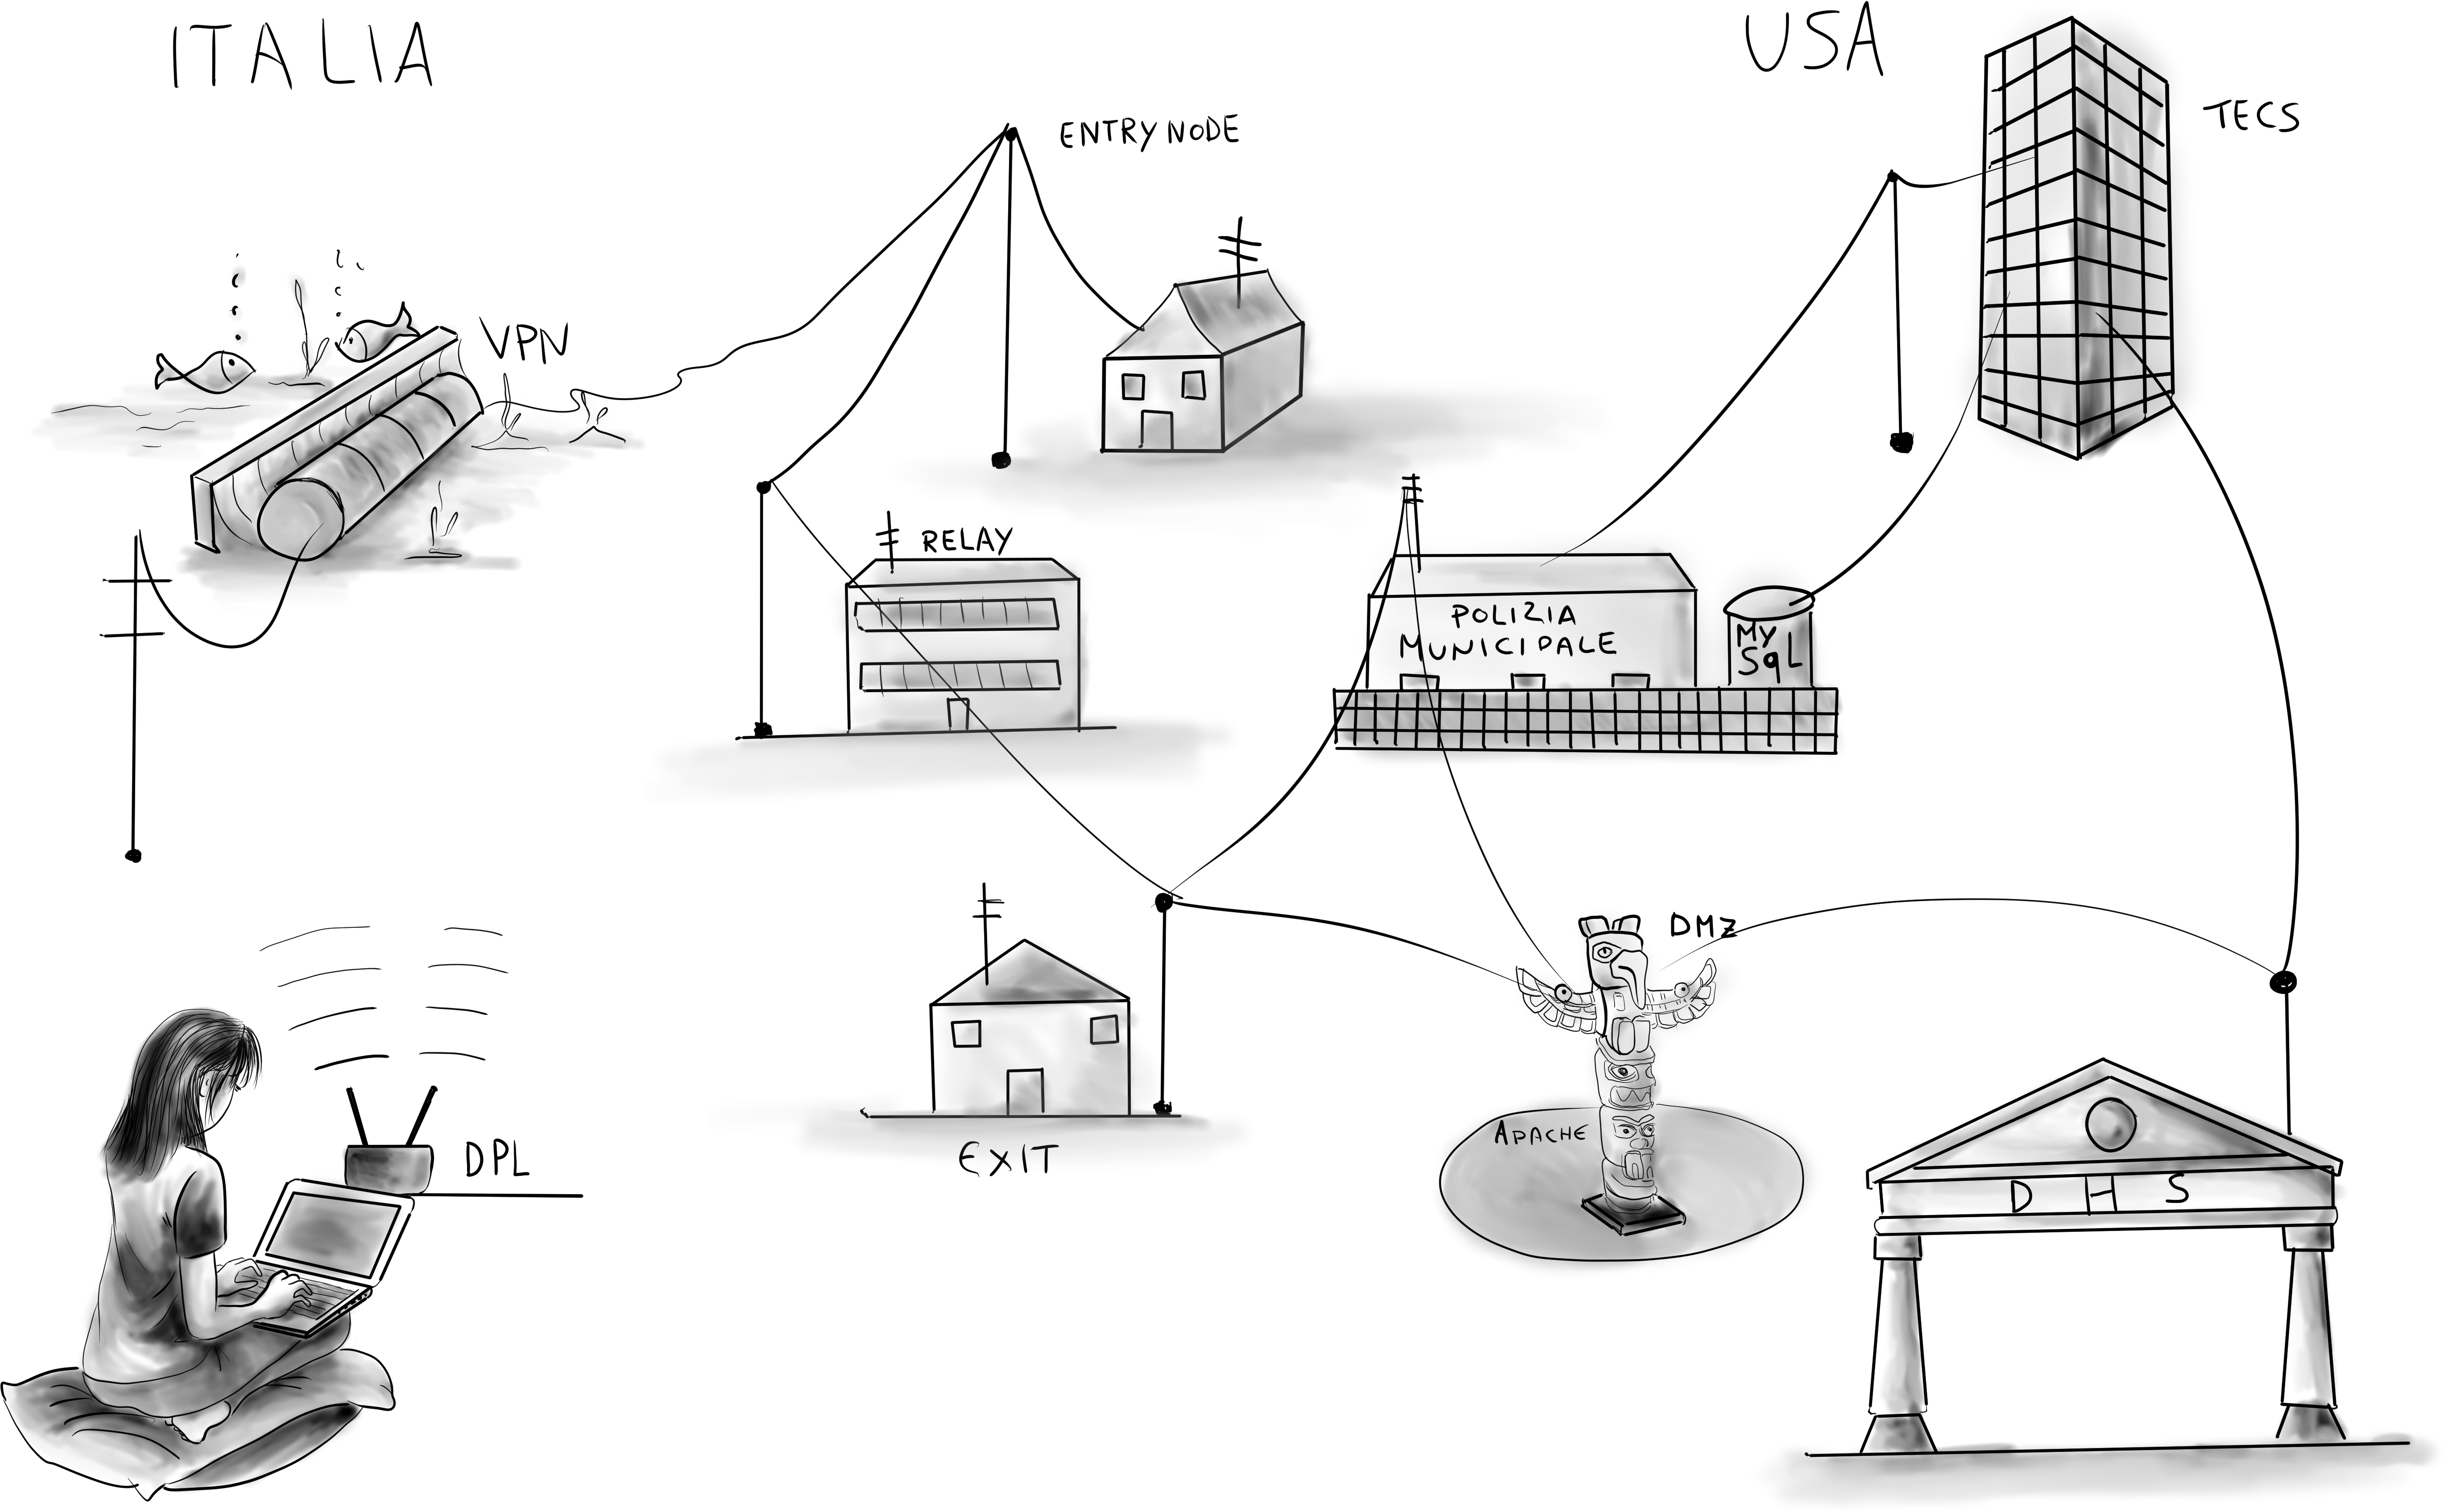
\includegraphics[width=.9\linewidth]{rete senza sfondo.png}
\end{center}

\par\medskip
«128 minuti per mappare l'infrastruttura e segnare i punti deboli. Prima una perlustrazione, vediamo le porte vintage. Se va bene trovo anche una SQL injection... Ce la possiamo fare, Rocky.»

\par\medskip
Allunga la mano, d’istinto, verso la cuccia.

\par\medskip
«Rocky? Dove sei, Rocky?»

% chapters/chapter06.tex
\chapter{Le regole del convitto}
«Muori Hanzaki!»\\
Giovanni schiva per un centimetro un fendente che finisce la sua corsa contro la scala.
«Sei lento, sei sempre stato lento... Non mi serve vederti, posso anticipare ogni tua mossa: questo è il segreto di Kage.»
\par\medskip
«Allora ferma questo colpo!» grida, e scatta brandendo il bastone sopra la testa.
\par\medskip
I due cani lo guardano avvicinarsi e raggiunge la giusta distanza, «Mi hai lasciato raggiungere \textit{ma-ai}, ora non potrai fermarmi.» I suoi movimenti si fanno prima lenti e poi  veloci, ma quando il bastone ha ormai raggiunto  Giovanni lui abbassa di poco la testa, alza le mani e rapidamente lo blocca.
\par\medskip
Osservandolo sembra che stia pregando. Ha le mani chiuse, palmo contro palmo, e in mezzo c'è il bastone, questo è un vera  contromossa ninja.
\par\medskip
\begin{center}
  \includegraphics[width=0.9\linewidth]{media/ma ai senza sfondo.png}
\end{center}

\par\medskip
Ipparchia si avvicina alla scena, lo sconosciuto depone il bastone e le accarezza il pelo sotto la gola. Giovanni accarezza invece la sua testa, scompigliandogli i capelli:
«Dai, adesso aiutami. Prendi il pacco, Luca. Hai visto come ho fatto tardi...»\\
«Infatti, ma questo cane? Dove lo hai preso?»\\
«Non lo so. Ha seguito Ipparchia.»\\
«E come si chiama?»\\
«Non lo so.»

\par\medskip
Luca si ferma e controlla:
«Ecco, è scritto sul collare, Rocky.»

\par\medskip
Rocky lo guarda.\\
«C’è un numero da chiamare?»\\
«Sì, è qui, guarda.»

\par\medskip
Passa qualche istante.\\
«Scusa, comunque c’è.»\\
«Bene, allora domani lo accompagneremo dai vigili. Ci penseranno loro. Portiamolo dentro per ora.»\\
«Lo leghiamo?»

\par\medskip
Giovanni attende. Non risponde subito.\\
«No, prima la libertà.»

\par\medskip
È un grande onore quello che Giovanni ha riservato a Luca: portare il pacco dentro al convitto. Certo, è Giovanni che ha fatto la strada maggiore, ma portarlo dentro significa qualcosa. Gli occhi nel buio lo scruteranno e sapranno che lui, Luca, ha portato il mangiare dentro.

\par\medskip
Però la strada è ancora in salita. Percorrere quella vecchia scala ferrata aggrappandosi con entrambe le mani è un conto; reggere in equilibrio quel pacco di viveri, cercando di non volare giù, è un altro. Ogni passo può tradirlo. La ruggine ha corroso i gradini e, un po’ per il buio, un po’ per il pacco che gli impedisce la vista, Luca deve andare a tentoni per non infilare il piede in una trappola.

\par\medskip
Giovanni, a questo, è abituato.

\par\medskip
«Cosa hai preso di buono, Giovanni?» gli domanda.

\par\medskip
«Una settimana di vita.»

\par\medskip
«Stai attento a non inciampare.»

\par\medskip
Quelle parole suonano quasi come una profezia.

\par\medskip
Un rumore secco, forse una sbarra che cede. Luca sta per perdere l’equilibrio.

\par\medskip
Giovanni si gira di scatto e lo afferra con precisione, evitandogli la caduta.

\par\medskip
«Wow!» esclama Luca. «Grazie!»

\par\medskip
«Tranquillo. Erano solo pochi metri. Però è sempre meglio evitare di cadere.»

\par\medskip
«Già.»

\par\medskip
«Eccoci.»

\par\medskip
Giovanni allunga una mano e trova a tastoni il telaio della porta finestra.

\par\medskip
«Siamo arrivati al primo piano. Aspetta...» Giovanni afferra qualcosa che gli sbarra la strada. Lo tira leggermente, poi ne tasta il contenuto: un carrello della spesa carico di stracci e prodotti per le pulizie blocca l’entrata.
Non è un carrello in buone condizioni. Mancano diverse sfere dai cuscinetti delle ruote, ma sarebbe comodo per portare la spesa. Ormai di carrelli non se ne trovano più. Giovanni però non ha mai pensato di usarlo a quello scopo.

\par\medskip
«Meglio salire al secondo piano» sentenzia.\\
«Ci sono, le pulizie?»\\
«Mi sa di sì.»\\
«Ok, saliamo.»\\
«Ci segue anche Rocky?»\\
«Sì, è dietro Ippa.»\\
«Speriamo non facciano storie… già si lamentano di lei.»

\par\medskip
«Dovrebbero essere in aula uno. Una volta entrati scendiamo dritti per lo scalone, non lo vedranno neanche.»\\
«Hai ragione.»

\par\medskip
Giovanni rallenta il passo per assicurarsi del terreno sotto i piedi, perché non conosce bene la seconda rampa delle scale. Entrare al primo piano è molto più semplice, ma adesso le casalinghe stanno facendo le pulizie, e a memoria di convitto, nessuno ha mai calpestato dove le casalinghe stanno pulendo.

\par\medskip
Sarebbe un errore irreparabile, perché significativo di ignoranza delle regole elementari di appartenenza a una comunità rispettabile. Basta riconoscere alcuni segnali elementari per non creare situazioni problematiche, e uno di questi è la presenza del carrello dei prodotti: un segnale universale di pulizia in corso. Impensabile spostarlo per passare.

\chapter{Missione per Rocky}

%Ha lasciato Valentina in casa da sola per cercare Rocky.\\
%Ma nei pressi di casa non lo trova.
%Adesso si trova di fronte a un dilemma: proseguire la sua intrusione etica ed aiutare l’amica nel poco tempo rimasto, o cercare il suo cucciolo prima che si ritrovi in qualche guaio?
«Rocky! Rocky!» il richiamo di Laura si perde nel silenzio, assorbito dalla boscaglia. Si allontana qualche metro, Valentina dorme, la zona è tranquilla, ma ha solo otto anni, pochi per restare in casa da sola. Torna in casa, il dog-contoller è lì, appeso alla parete ormai da mesi, non è al collo dove dovrebbe essere: «Non sono stata brava.»\\
Torna dentro, riempie la ciotola con un po' di croccantini: «Vediamo così.» Percorre il perimetro della casa agitando la ciotola e chiamandolo. Niente. «Dove è andato?» Un barlume: «Il chip del canile. Potrebbe aver lasciato delle tracce.»


\par\medskip
«Cate, ho bisogno di un favore. Rocky è scappato.»\\
«Oddio, quando?»\\
«Non lo so. Forse quando sono entrata per prenderti la giacca. Comunque devo andare a cercarlo. Però ho bisogno per Vale, non posso lasciarla da sola in casa.»\\
«Certo. Dammi dieci minuti che arrivo.»

\par\medskip
«Dove ho messo il codice...» Laura cerca il documento di Rocky, dal codice identificativo potrà verificare se qualche scanner urbano ha rilevato il suo chip e provare a ricostruire la posizione.\\
«Eccolo! Vediamo se c'è anche un indirizzo...»
\begin{terminalbox}
kali@dpl:~$ telnet gates.ith56.it 2323
Trying 203.0.113.57...
Connected to gates.ith56.it.
Escape character is '^]'.

ITH56 urban-gates legacy console
login: laura
Password:

laura@gates-legacy:~$ CHIP=1889
laura@gates-legacy:~$ grep "$CHIP" dog-registry.log | tail -n 5
laura@gates-legacy:~$ tail -F dog-registry.log | grep --line-buffered "$CHIP"
laura@gates-legacy:~$ grep "1889" dog-registry.log | tail
 gate=ITH56-T3-017 reader=rfid-a03 chip=1889 rssi=-67 direction=OUT
 gate=ITH56-T3-019 reader=rfid-b01 chip=1889 rssi=-72 direction=OUT
$
\end{terminalbox}

I dispositivi RF-id lasciano tracce digitali, quelle degli animanli sono liberamente accessibili. In passato diverse applicazioni utente usavano questi dati, ora la gente preferisce i collari di controllo. Laura ha trovato il file con i dati, e lì le tracce di Rocky. Il computer però è scomodo, non può usarlo in azione. Rocky si sta muovendo, lo vede dall'aggiornamento dei dati, per ritrovarlo dovrà agire, incrociare i dati del registro con la posizione GPS dei varchi urbani.


Sono passati tredici minuti, Caterina e Alice atterrano. Laura sente il rumore, va loro incontro: «La porta è aperta,
\par\medskip
Un cane in un territorio misto può perdersi ovunque: da una linea abbandonata della metro a un centro di assistenza per l’intelligenza artificiale. Comunque, a quanto risulta, dal suo segnalatore non è andato troppo lontano. Sembra essere in un boschetto a poche centinaia di metri.

\par\medskip
I problemi si risolvono creando ordine: Laura sistema il suo zaino tattico perché il suo contenuto determinerà il successo della missione. Come a scuola: infilare nello zaino il quaderno sbagliato potrebbe compromettere la giornata!\\
– una corda in microfibra nano tessuta,\\
– una carrucola smart a riduzione di carico,\\
– guanti grip GECO,\\
– un micro drone da zaino con telecomando e telecamera termica,\\
– un visore Augmented Reality multifunzionale,\\
– sfere da esplorazione,\\
– spray a schiuma rapida,\\
– una batteria al grafene ultracompatta,\\
– una radio Mesh Network autonoma e un beacon personale,\\
– infine un esoscheletro pieghevole e una barella smart ultracompatta.

\par\medskip
Alice la osserva ammirata: Laura nella sua tuta nera.
\par\medskip
«Sembri Tomb Rider! Ma cosa c’è nello zaino?»\\
«Niente, amore, ho preso i suoi croccantini per chiamare Rocky.»
\par\medskip
Non mente, ci sono anche i croccantini.
\par\medskip
«Dovrebbe essere qui vicino. Farò presto.»\\
«Laura, posso venire con te? Può restare Alice con Vale?»\\
«In effetti…»\\
«Sì, ci penso io.»
\par\medskip
Caterina indossa una minigonna, una camicetta e un paio di scarpette con un po’ di tacco.  
Ha un abbigliamento perfetto per quello che le attende.
\par\medskip
«Ok, mi raccomando, Alice.»
\par\medskip
Alice non risponde. Sorride, entra in casa e le guarda dalla vetrata.

\par\medskip
Prenderanno il drone? No, sembra si avviino a piedi lungo la capezzagna.  
Qui ci sono già passate insieme, quella sera, prima della loro avventura nel computer quantistico.  
Sì, quella è stata davvero una bella sfida: la posta in gioco era alta, la libertà di essere decoerenti.  
Ma ora la questione è altrettanto seria.

\par\medskip
La strada termina in un incrocio a T.  
Il sensore indica che Rocky si trova davanti a loro a circa ottanta metri, non a destra e non a sinistra.

\par\medskip
\begin{center}
  
\includegraphics[width=1\linewidth]{piantina rocky senza sfondo.png}
\end{center}

\par\medskip
«Dovremo entrare nel campo?»\\
«Se procediamo e prendiamo qui a sinistra, seguendo la strada, ci possiamo avvicinare un po’.  
Ma alla fine credo che dovremmo comunque entrare. Rocky mi sembra in mezzo al campo.»

\par\medskip
«Di quanto la allunghiamo?»\\
«Circa seicento metri, direi. Solo cinque minuti. Cosa ne dici?»\\
«Forse era meglio venire con il drone?»\\
«Rocky ha paura dei droni, Cate, sarebbe stato peggio.»\\
«Dai, decidi tu allora, Laura.»\\
«Beh, allora avviciniamoci seguendo la strada, poi valutiamo.»\\
«Cosa dice la posizione?»\\
«Sembra fermo, speriamo stia bene, non rilevo i parametri biometrici.»\\
«Cosa significa, Laura?»\\
«Ma niente, mi sa che semplicemente non ho rinnovato l’abbonamento.»\\
«Qui svoltiamo a destra.»\\
«Ehi! È messa male questa strada.»\\
«Tutta l’area ormai è un po’ andata.»\\
«Ecco, di nuovo a destra e tra un centinaio di metri dovremmo esserci.»\\
«Non siamo mai venute qui insieme, vero?»\\
«No, ci siamo fermate alla panchina. Comunque anch’io erano anni che non facevo questa strada.  
Forse l’ultima volta sono venuta con mio padre, poco prima che nascesse Valentina.»\\
«A proposito, chissà come se la cavano quelle due.»\\
«Dietro il cespuglio c’è un cancello, ma non mi risulta nella mappa.»\\
«Comunque Rocky dovrebbe essere qui a trenta metri, solo che non vedo come entrare.»\\
«Vediamo se c’è un varco. Qui, Laura.»\\
«Grazie, Cate, sono contenta che tu sia venuta con me.»\\
«Dai, proviamo a entrare.»\\
«Aspetta, ma c’è una scritta: Convitto Cardinal Mora.  
Lavori di ricostruzione. Ma la data è del 1970! Ecco perché non è più nella mappa.»\\
«Quindi Rocky sarà qui dentro.»\\
«Ora lo scopriamo.»

\par\medskip
Laura e Caterina superano il confine tra il presente e questo mondo che appartiene a un passato dimenticato.

\par\medskip
Riusciranno a uscire indenni anche questa volta?

\chapter{Il tranello della mensa}

\par\medskip
«Passiamo per la palestra e raggiungiamo le scale.»\\
«Va bene, Luca, fai tu strada.»

\par\medskip
I quattro imboccano la stessa scorciatoia che usavano le ragazze per scendere in mensa senza farsi vedere dai maschi quando il convitto era ancora attivo. La porta finestra di emergenza da cui sono entrati si apre infatti nell'ex camerata femminile e, da lì, un'uscita laterale conduce a un corridoio sul quale si affaccia una delle due porte della palestra. L'altra dà direttamente sul pianerottolo delle scale.

\par\medskip
Giovanni procede con cautela. Nella camerata ci sono ancora letti semidistrutti e materassi lasciati alla rinfusa sul pavimento, ostacoli da superare senza fare troppo rumore. Per fortuna Ipparchia e Rocky li seguono senza abbaiare, ma il loro obiettivo di segretezza sembra appeso a un filo.

\par\medskip
Luca gli afferra la mano.

\par\medskip
«Passiamo di qua.»

\par\medskip
Pochi passi ancora e raggiungono il corridoio.

\par\medskip
Una luce tremolante filtra dalla palestra. Proviene da un bidone di latta: uno stoppino fatto di stracci imbevuti di olio esausto continua a bruciare lentamente.

\par\medskip
Giovanni annusa. Conosce bene quell'odore. Ogni tanto scende dal secondo piano e gli pizzica il naso.

\par\medskip
Non gli piace.

\par\medskip
È sintetico, acre, tossico.

\par\medskip
Però fa luce.

\par\medskip
E la luce, a lui, non serve.

\par\medskip
\par\medskip
«Un attimo...»

\par\medskip
Luca controlla che tutti lo abbiano seguito, poi appoggia il cartone a terra per sistemarsi la cintura. Fatto questo, ripartono.

La porta della palestra è aperta. Anzi, la porta non c'è più da anni. Il varco però è inconfondibile: dove prima c'era un battente, ora si apre un portale di luce soffusa e suoni attenuati.

Dall'interno arrivano musichette elettroniche, jingle brevi e chiptune  di vecchie console. Anche quei suoni sono familiari a Giovanni, sorride alle frasi corte e simmetriche del Pac-Man, ripensando a quando studiava i percorsi di fuga seguiti dal ghost-team quando Pac-Man mangiava una delle pillole energetiche.

\par\medskip
Entrano con cautela. Nella palestra diversi ragazzini tengono in mano joystick e controller e giocano davanti a monitor recuperati.

\par\medskip
Luca li saluta con un cenno, ma non si ferma.

\par\medskip
L’attenzione di tutti è verso Rocky: la curiosità è alta, ma nessuno lascia la console, anche se gli occhi vanno e vengono dal cane.

\par\medskip
Attraversano l'ex palestra fino a raggiungere la seconda porta.  Nella mappa mentale che  Giovanni  sta tracciando, le due porte sono allineate creando una particolare connessione  che permette di entrare nella palestra da una porta e uscire dall'altra. Se  loro fossero in un videogioco di quelli in esecuzione nelle console, come il Pac-Man attraversandola si ritroverebbero al punto di partenza. Ma non è così, e quando attraversano il portale nel verso opposto  l'aura rosa azzurra che rifletteva suoi loro volti li abbandona e tornano ad essere  ombre scure nel convitto. Raggiungono il pianerottolo. Luca si avvicina all'amico: «Stai attento per le scale, ci sono diversi buchi».

\par\medskip
\begin{center}
  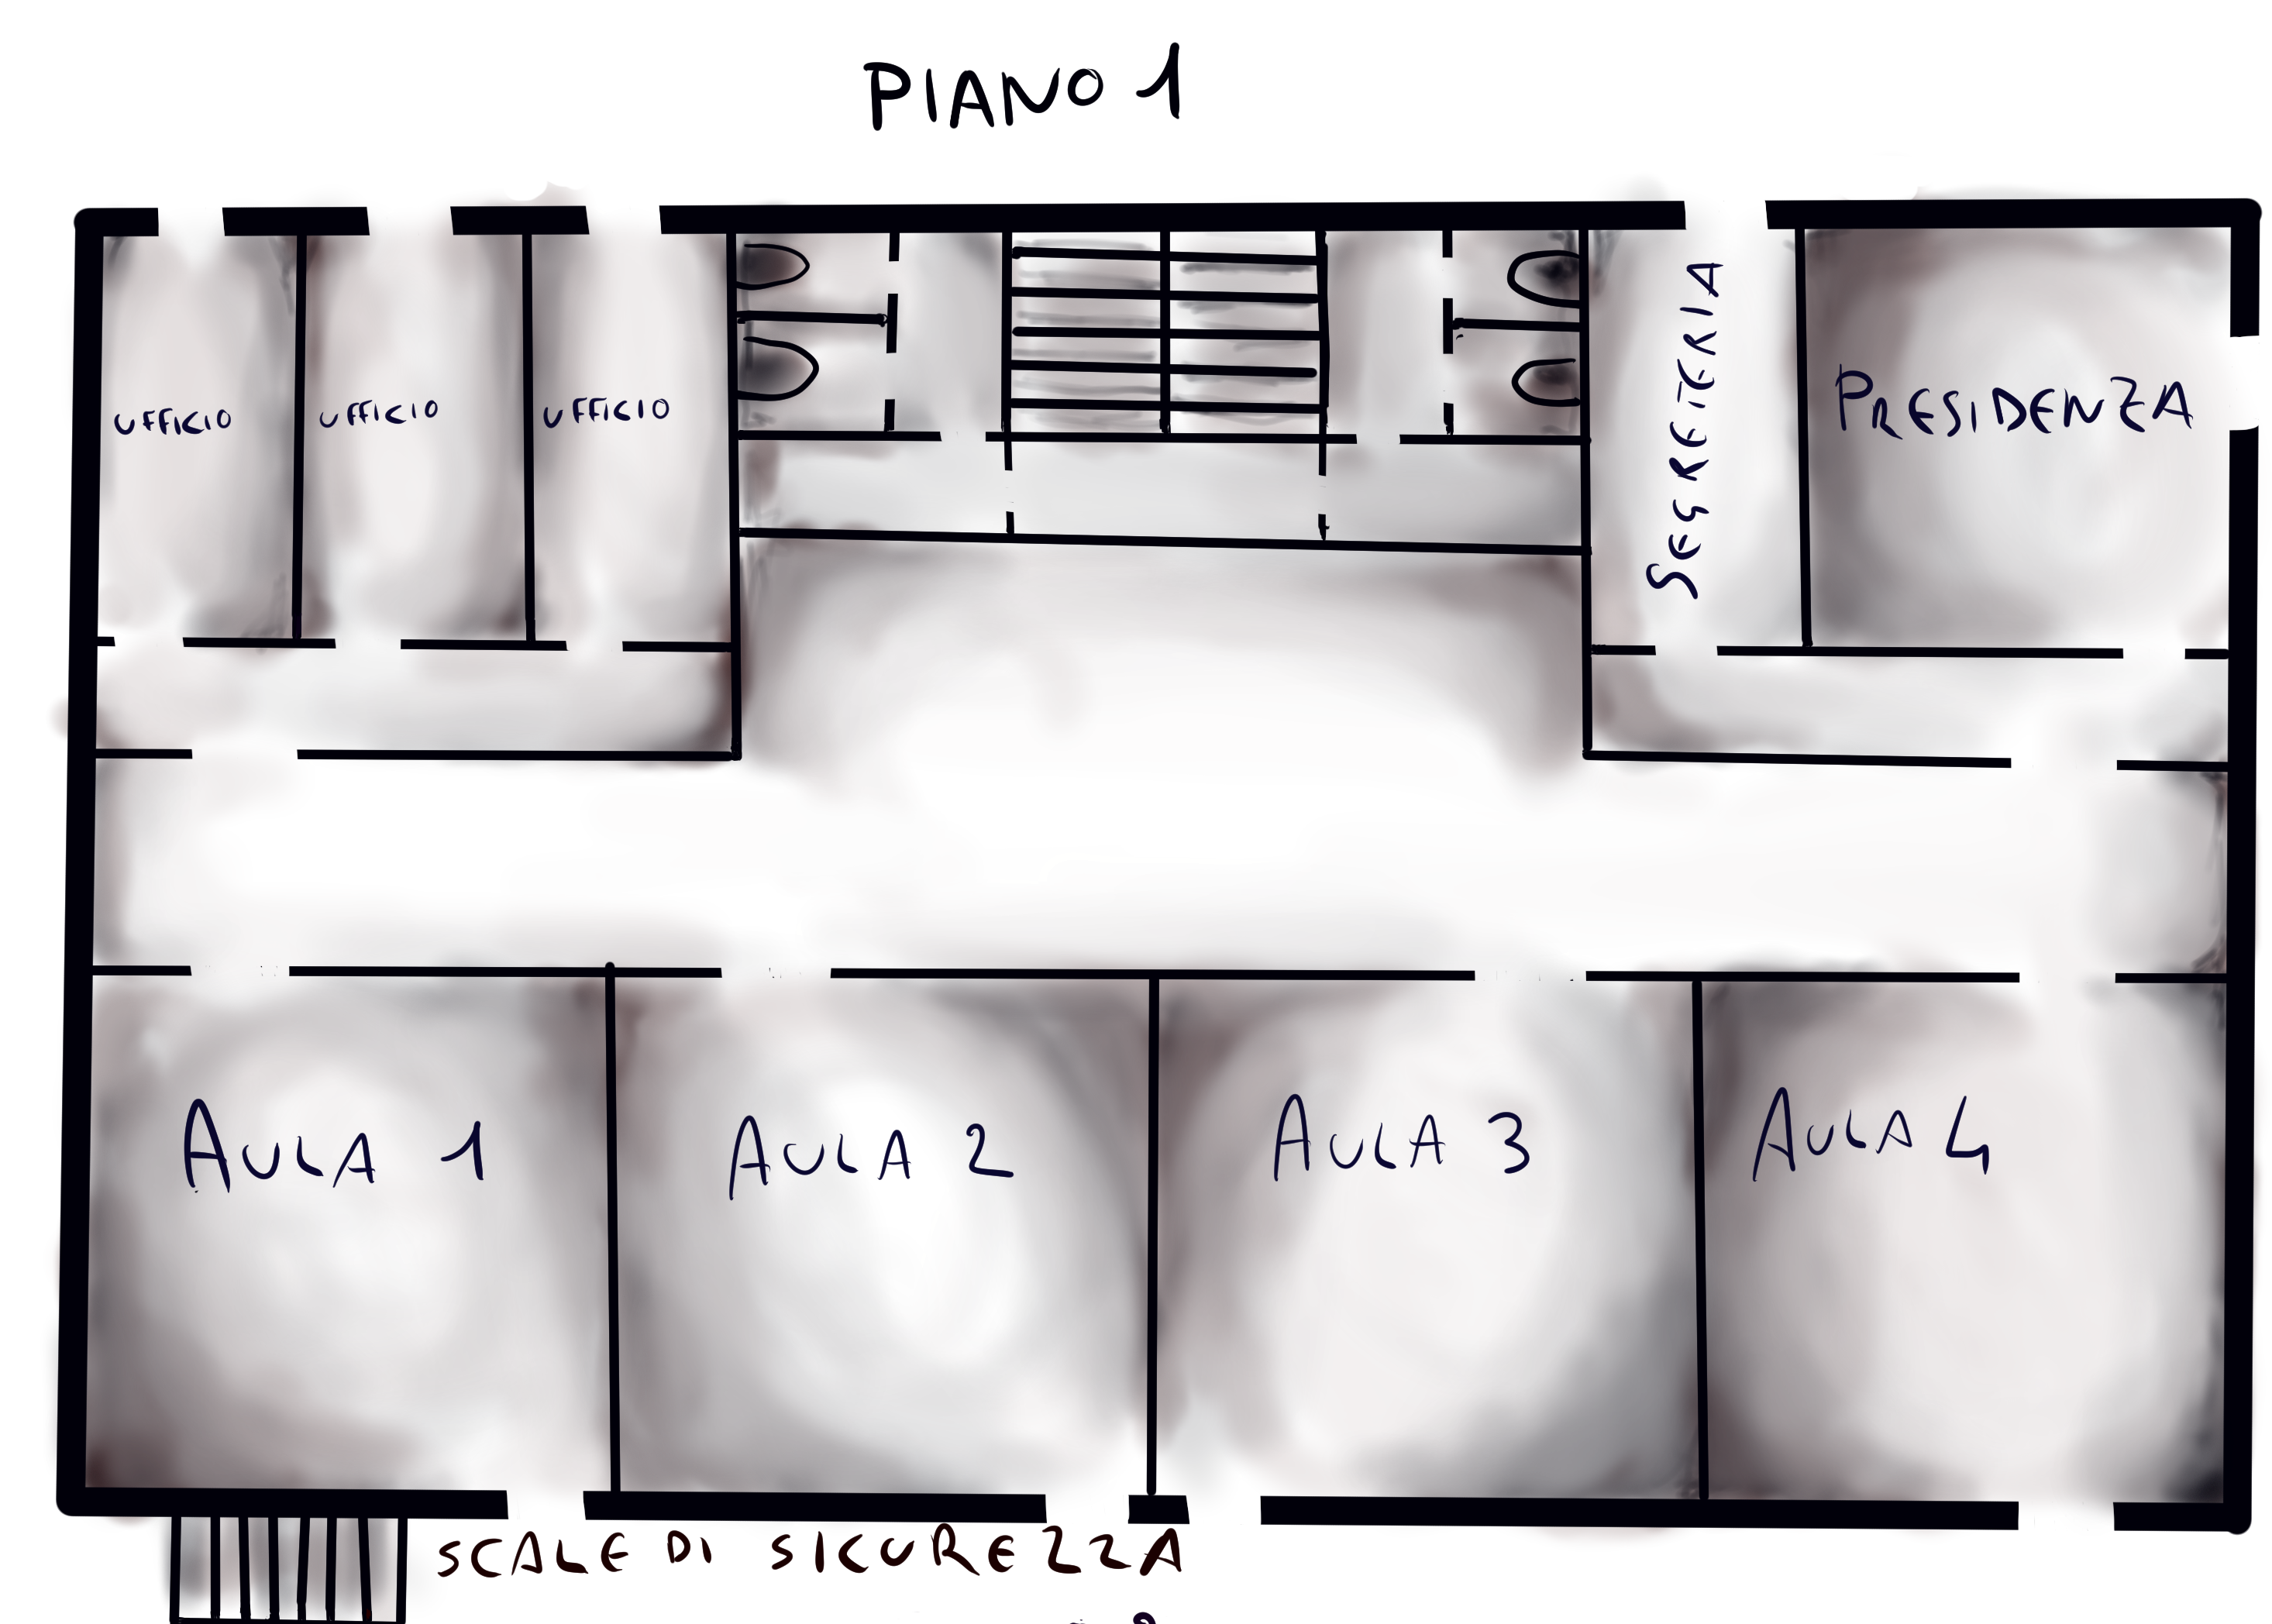
\includegraphics[width=1\linewidth]{piano 1.png}
\end{center}

\par\medskip
\begin{center}
  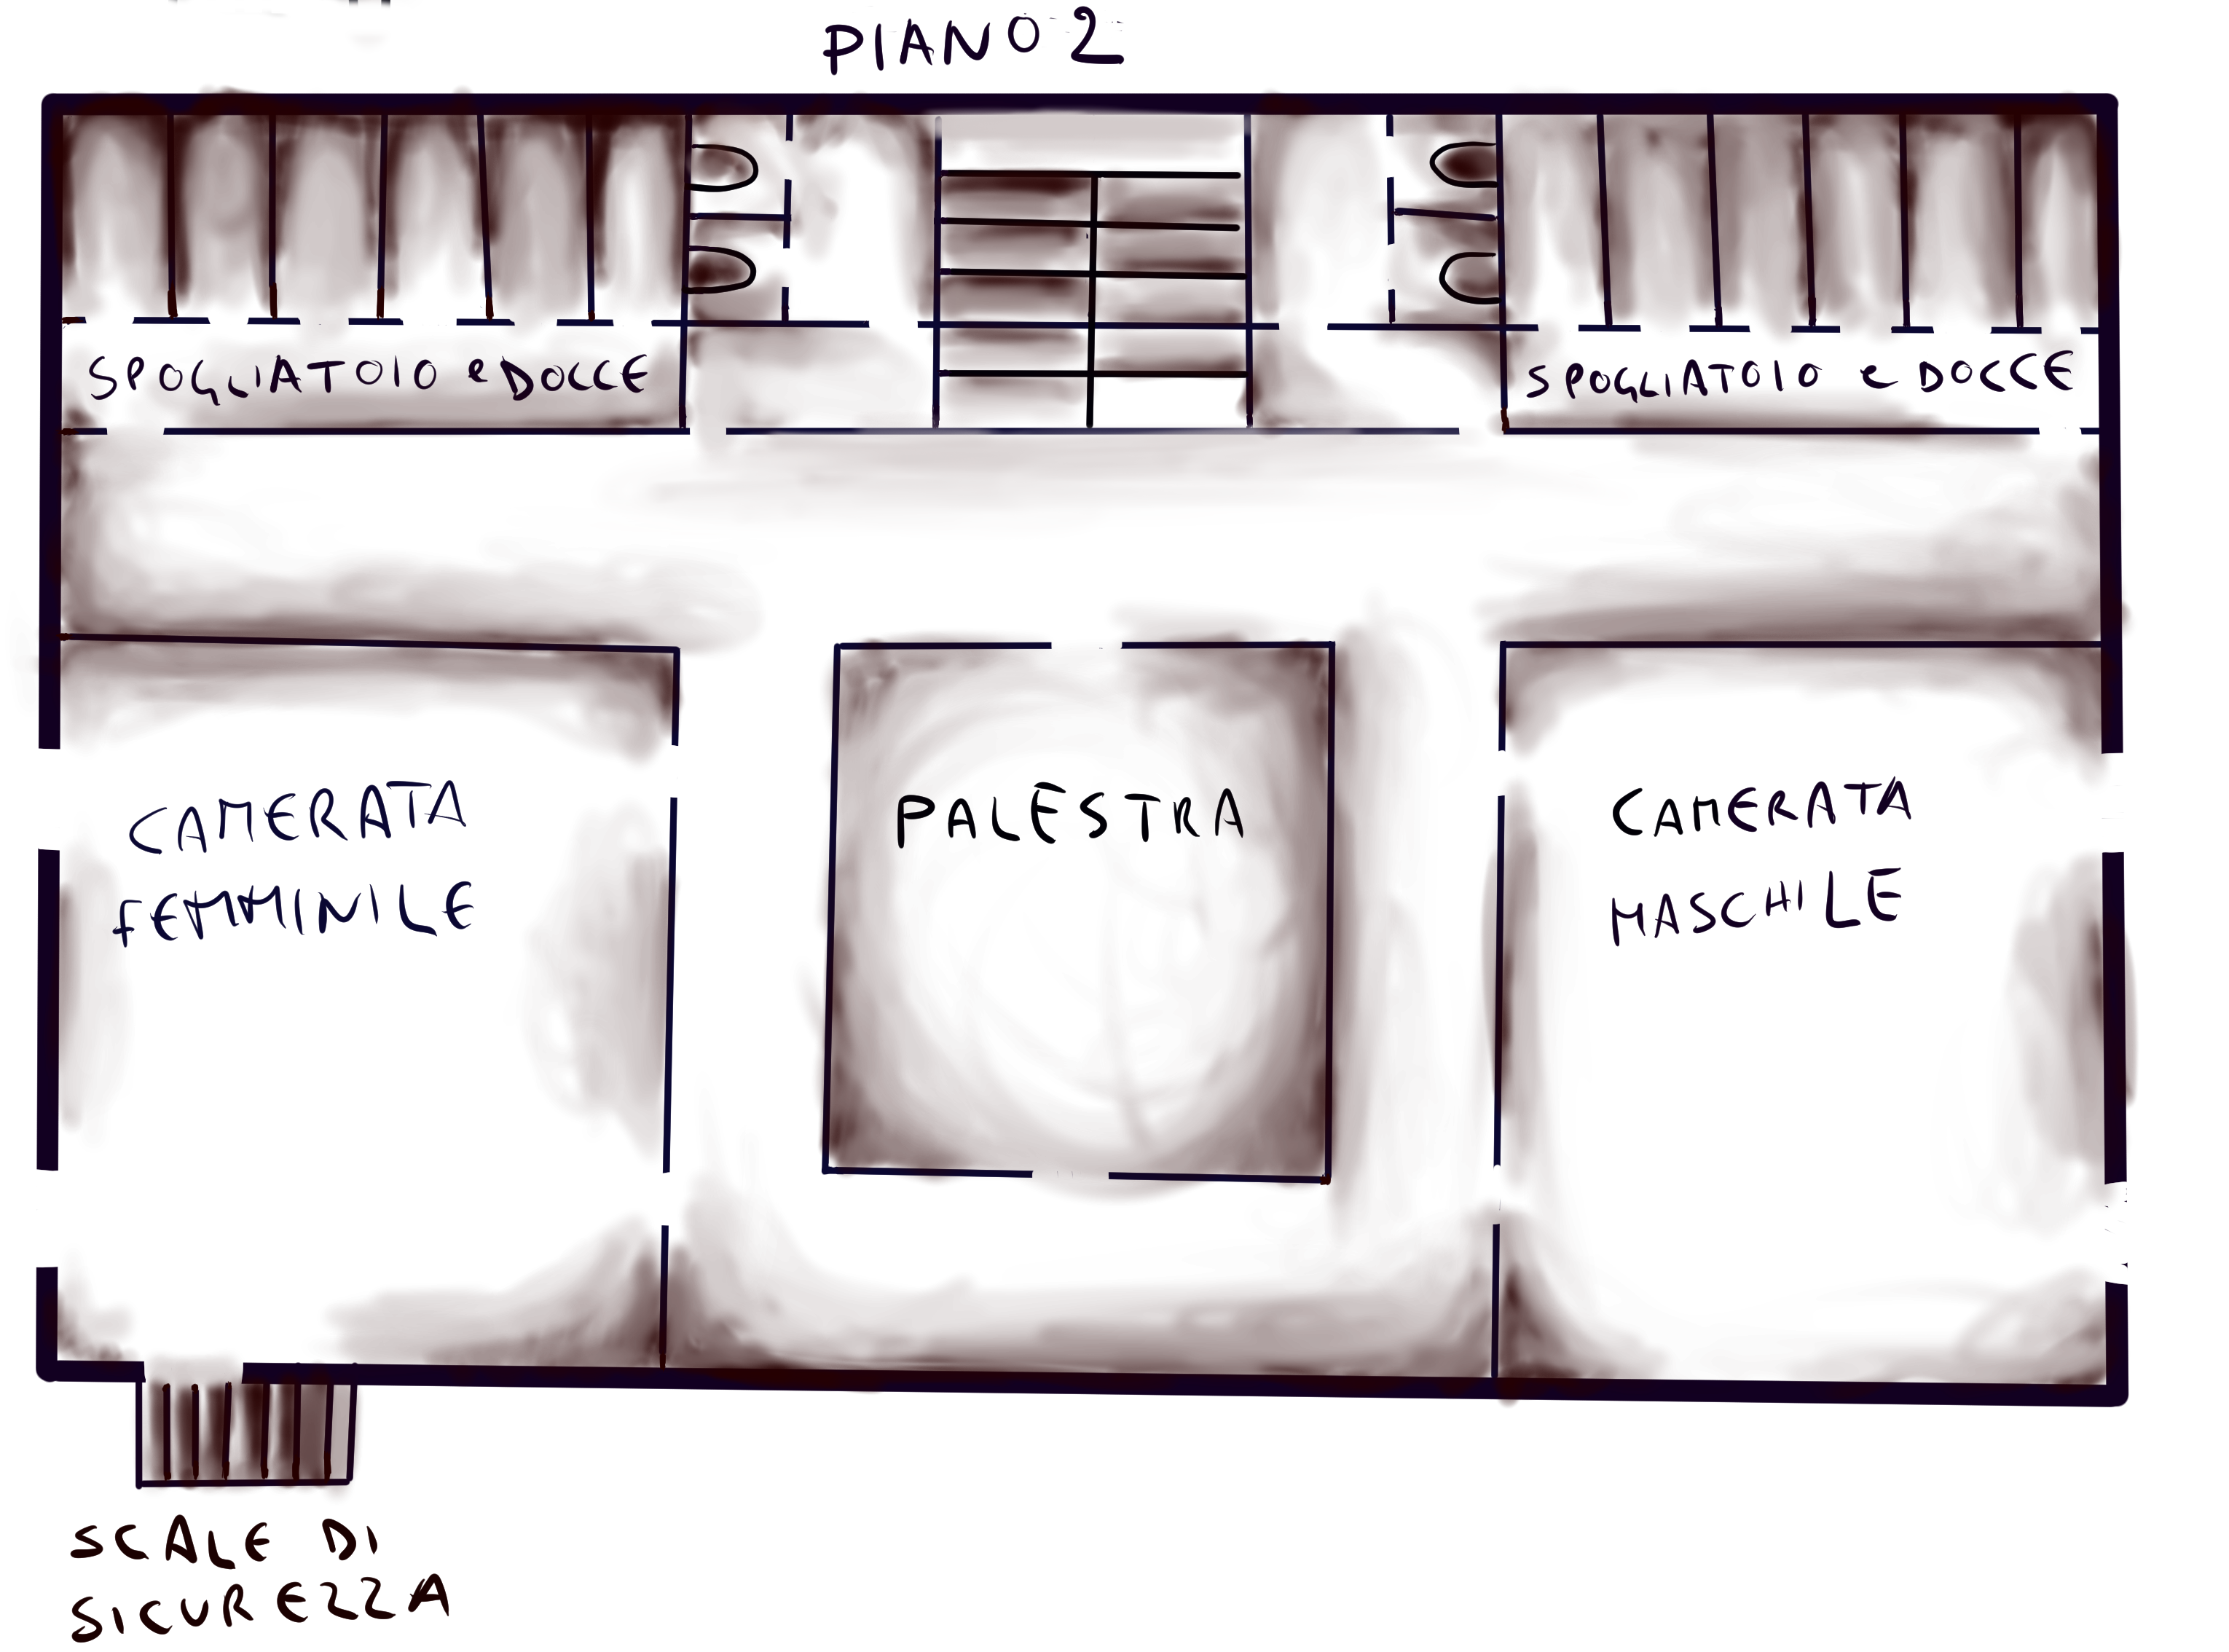
\includegraphics[width=1\linewidth]{piano 2.png}
\end{center}

\par\medskip
Giovanni si tiene radente al muro e misurando i passi uno ad uno raggiungono il primo piano.  Li la presenza delle casalinghe è palpabile o udibile due concetti analoghi quando l'udito è il primo dei sensi. il ritmo quasi isterico con cui gli oggetti vengono presi, puliti e riposti è una traccia inconfondibile. Tutti i piani sono soggetti alle loro cure, ma sempre uno alla volta a partire dal piano terra salendo fino al secondo. Comunque sono tutte nelle indaffarate nelle aulee, così  basta passare in un attimo: leggeri come il vento e continuare a scendere le scale.

\par\medskip
In mezzo alla rampa c’è un buco. Giovanni lo sa.  
È radente al muro perché conosce quel buco.

\par\medskip
Per un attimo pensa a Rocky, ma anche lui è e rimane radente al muro.

\par\medskip
Per ora nessun problema.\\
Un’altra rampa e raggiungono la Hall al piano terra.

\par\medskip
\begin{center}
  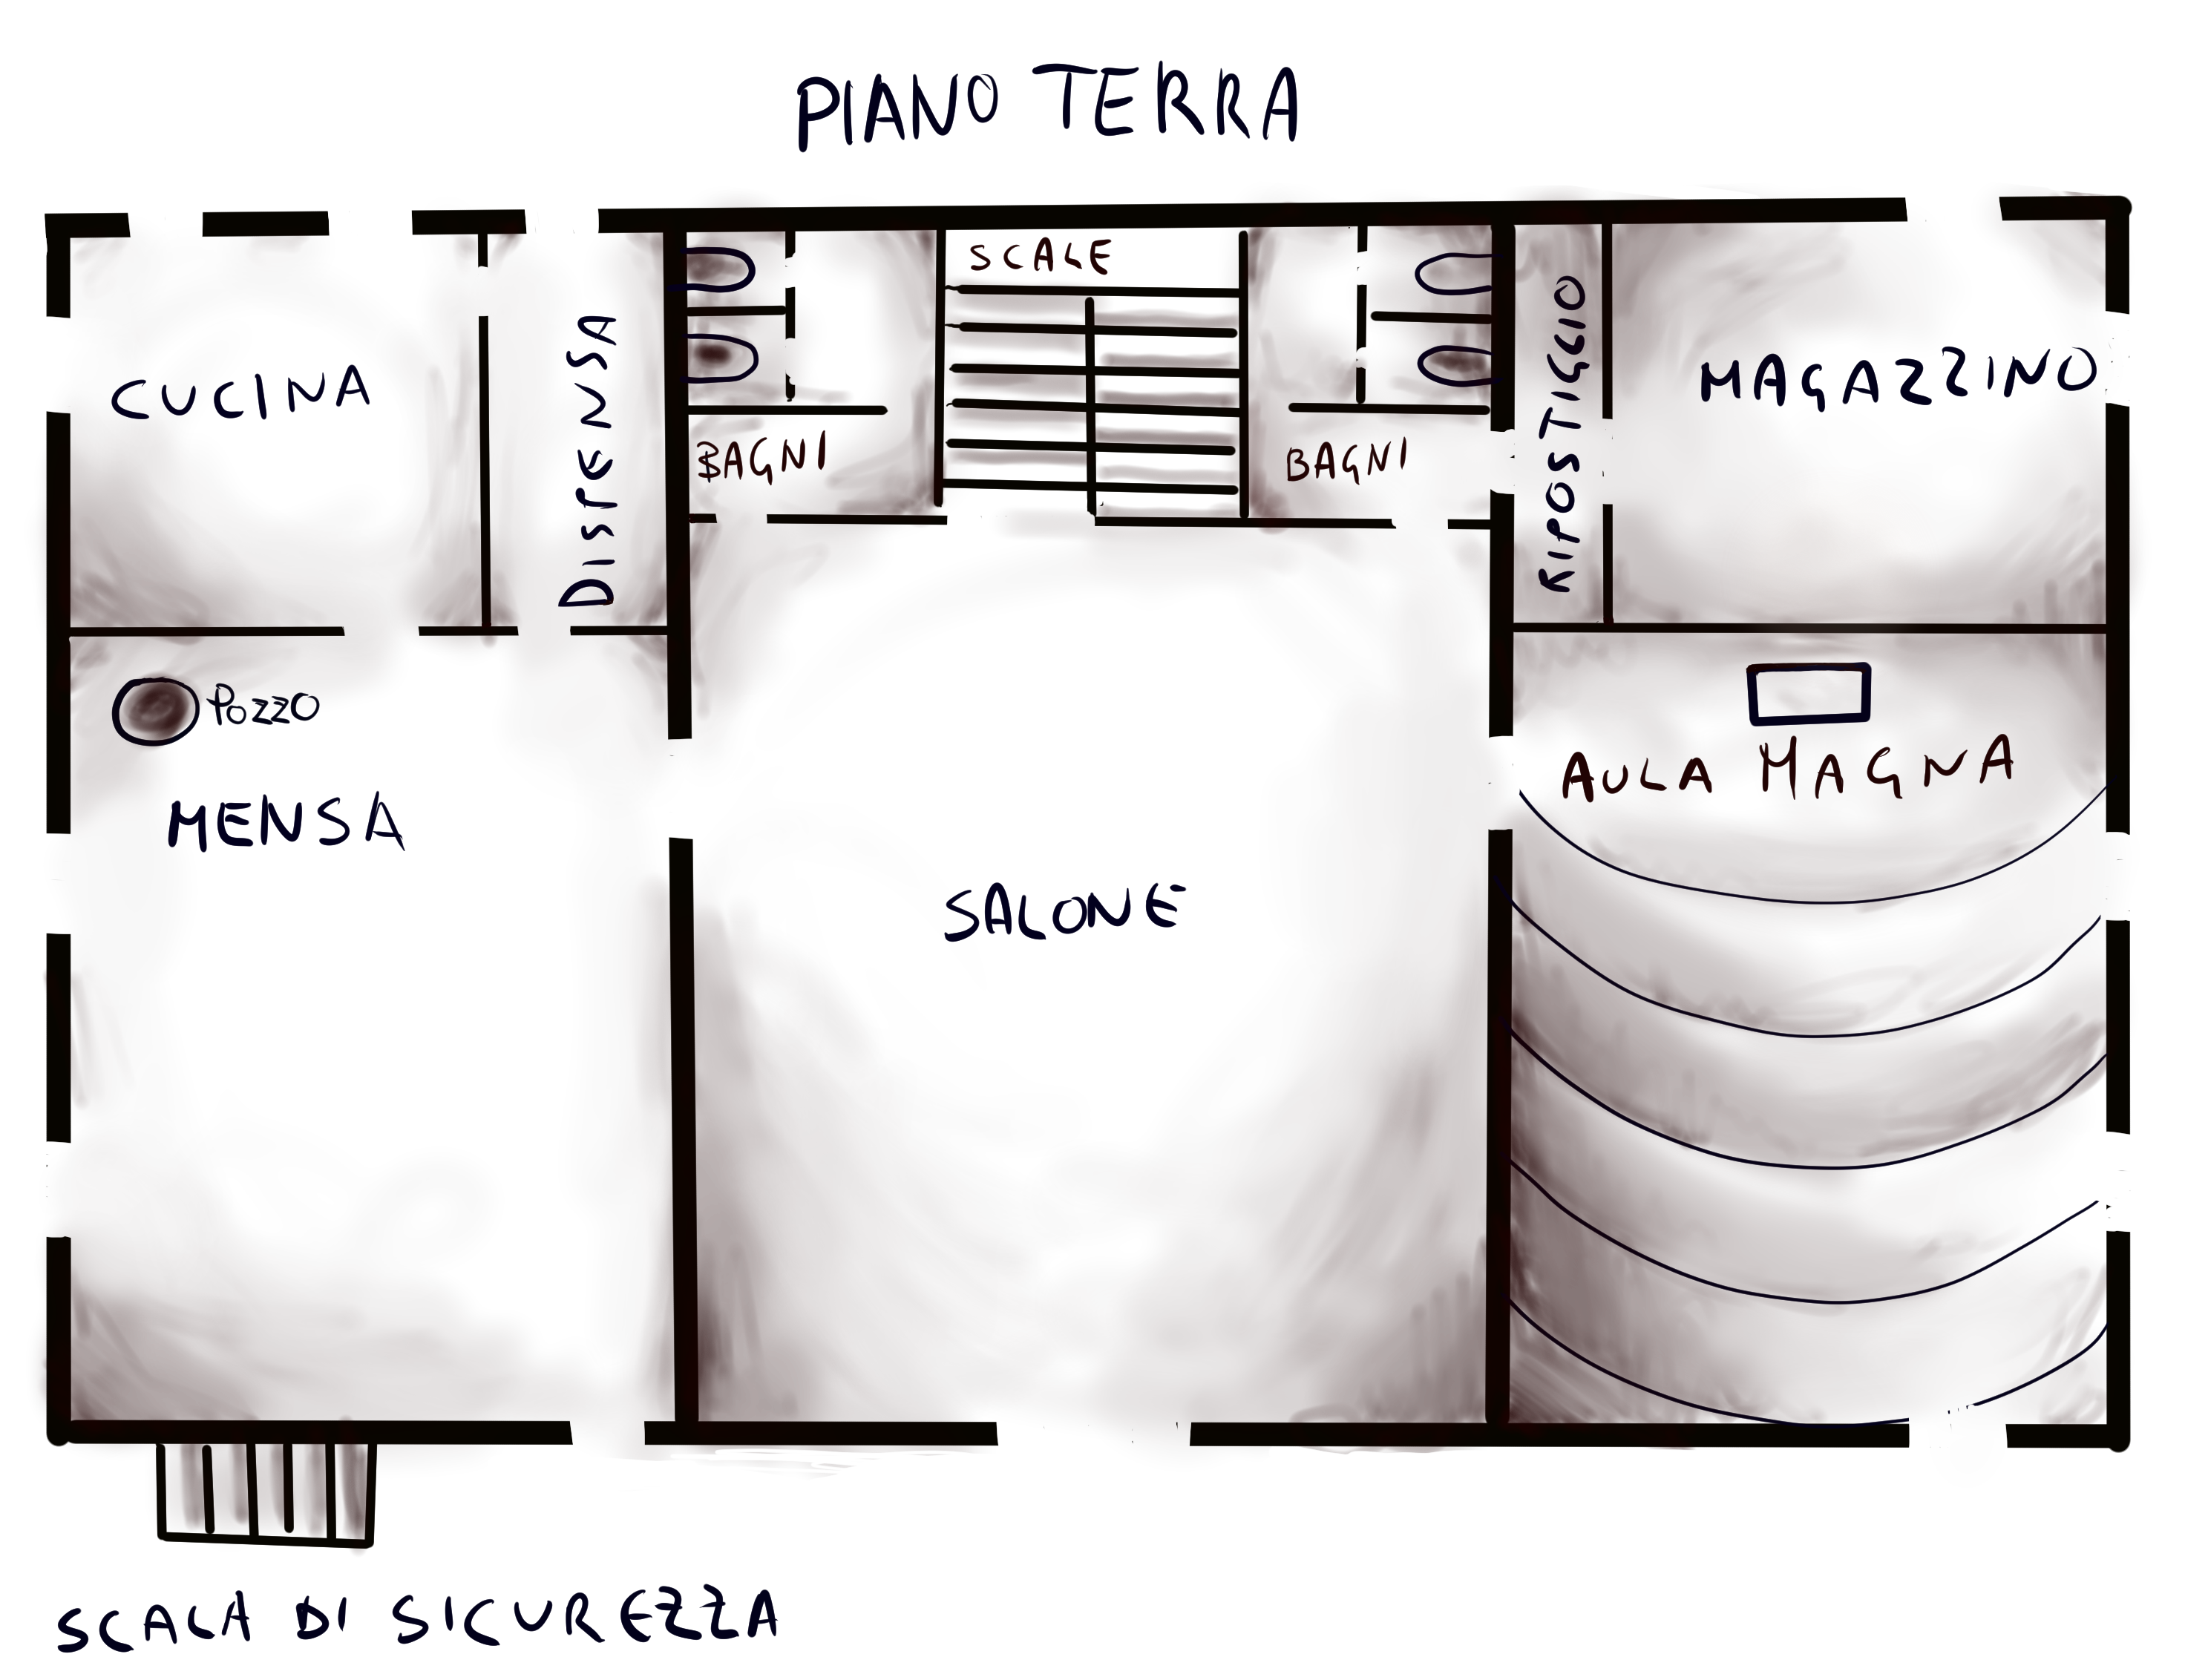
\includegraphics[width=1\linewidth]{piano terra.png}
\end{center}

\par\medskip
Qui Giovanni si muove sicuro, punta dritto alla porta della ex Mensa, mentre Luca lo segue con affanno.  
Il pacco comincia a farsi sentire.

\par\medskip
Rocky si guarda intorno. I cavalletti devono sembrargli ottimi per una pausa pipì, ma per fortuna non ne approfitta.

\par\medskip
Una candela è accesa. Qualcuno sta già mangiando.  
Ippa non cede al richiamo dell’odore, ma Rocky non è ancora altrettanto disciplinato.  
Si distacca dalla comitiva e va verso il tavolino.

\par\medskip
Luca lo guarda.\\
«No, Rocky, fermo!»

\par\medskip
È rapido. Non è ancora un ninja, ma ha la prontezza di lasciare andare i beni sostituibili per provare a salvare una vita non sostituibile.  
Il pacco cade mentre lui si lancia per afferrare il nuovo amico.

\par\medskip
Dopo sessanta secondi la situazione è questa: in mensa è rimasto solo Giovanni.  
Chi altro c’era si è dileguato.

\par\medskip
Luca è vigile e cosciente, ma malamente incastrato non riesce a far forza per risalire.  
Giovanni parla con lui mentre Rocky abbaia.

\par\medskip
«L'acqua mi arriva alla bocca. Non riesco a tenere su la testa.»\\
«Stai tranquillo, non salirà di livello.»\\
«Sì, sì.»\\
«Ci sono io, ti faccio uscire.»

\par\medskip
Giovanni chiama ancora aiuto, ma anche qui nel convitto le cose sembrano andare come fuori.

\par\medskip
«Vado a chiamare qualcuno. Torno subito.»\\
«Non lasciarmi da solo!»\\
«C’è Rocky, arrivo subito.»

\par\medskip
Ippa lo segue. Corre nella hall e poi verso l’entrata principale.  
Solleva la barra e si fa giusto lo spazio per passare.

\par\medskip
«Ehi amico, che passa?»\\
Una voce lo coglie appena si fa fuori.\\
«Ho bisogno. Uno dei ragazzini è finito nel pozzo.»

\chapter{Intrappolate}

«Ahi, mi sono graffiata.»\\
«Di qua, Cate, c’\`e un passaggio.»\\
«Ah, ma perch\'e ho sempre la gonna? Arrivo, Laura.»\\
«Certo che questo giardino non vede un giardiniere da un bel po’ di tempo.»\\
«Giardiniere? Qui ci vorrebbe... non farmelo dire, non sarebbe ecologico. Guarda, l\`i c’\`e un bidone con una rete. Forse ci vive qualcuno?»\\
«Non lo so, questo edificio non \`e neanche sulla mappa. Andiamo a vedere. Rocky dovrebbe essere vicinissimo ormai.»\\
«Il bidone \`e caldo, qualcuno dimora qui. Cosa facciamo, Laura? Rocky potrebbe essere dentro, proviamo a chiamarlo?»\\
«\`E meglio di no. Se c’\`e qualcuno, potremmo mettergli paura, farlo scappare e Rocky con lui. Capiamo se riusciamo a guardare dentro e se c’\`e un punto di accesso sicuro.» Laura si leva lo zaino e prende il drone da rilevamento.
«Cosa fai?»\\
«Cerchiamo un accesso con il drone.» Attiva il drone e fa un volo di prova.
«Ma la porta \`e un po’ aperta, mi sembra.»\\
«Non va bene, ci serve un’entrata che non ci faccia notare. Meglio non rischiare.»

\par\medskip
Caterina si avvicina alla scala antincendio, afferra il corrimano e lo scuote. L'intera struttura vibra e risuona alla sua manovra. Appoggia un piede sul primo gradino. I successivi presentano ferri sporgenti e qualche fessurazione.
«Laura, qui, vieni», le sussurra.

\par\medskip
«Cate, sei gi\`a salita!» Laura spegne il drone e lo riaggancia allo zaino.\\
«Coraggio, seguimi.»

\par\medskip
Caterina avanza per le scale, il tacco ogni tanto si intrappola tra le grate delle scale, ma sembra non curarsene troppo. Laura la segue con passi misurati, senza fare rumore. L'amica si volta verso di lei:
«Hai assolutamente ragione a non entrare nella porta principale. Non stiamo entrando in una proprietà privata» le sussurra con una punta di complicità: «Questo \`e proprio un altro ecosistema, e la prima regola \`e: non perturbarlo» si interrompe: «...ma guarda dove  c’\`e un carrello della spesa!»\\
Con gesto deciso lo spinge via.\\
«Ecco, adesso il passaggio \`e libero» sussurra, divertita. «E senza esserci fatte notare.»

\par\medskip
Laura la raggiunge sul pianerottolo che si piega leggermente: «Non sembra regga bene...»\\
\`E buio ma superano la portafinestra e sono dentro. Laura afferra l'amica per un braccio:
«Fermiamoci un attimo.» Si leva lo zaino, sgancia il drone e dalla tasca laterale sinistra prende il controller.\\

«Cosa vuoi fare?» Caterina le sussurra vicino all'orecchio: «Siamo gi\`a dentro, no?»\\
«Lo attivo comunque. Potrebbe servirci.»\\
\par\medskip
Il LED RX  lampeggia: «Niente connettività, solo registrazione locale. Non basta per la mappa 3D», sussurra.\\
«Qualche problema?»\\
«Non proprio. Avrei voluto costruire una mappa 3D, ma non c'\`e connessione al satellite.»\\


«Wow, Laura! Volevi una mappa di questo posto in 3D? \`E fantastico, ma non sarebbe meglio se cercassimo subito Rocky?»\\
«Hai ragione, forse sono troppo prudente»

\par\medskip
Improvvisamente arriva un latrato poi un urlo, una voce maschile\\
\par\medskip
\begin{center}
  
\includegraphics[width=0.7\linewidth]{media/equipaggiamento laura senza sfondo.png}
\end{center}

«Questo \`e Rocky» Attende un istante, poi riprende:  «Sembra venga da sotto. Andiamo a vedere.»\\
«Ma hai sentito quella voce?»\\
«Sì l'ho sentita, adesso sappiamo che non siamo sole di sicuro.» Laura avanza, la stanza \`e buia, lentamente si fanno strada tra una distesa di scranni e  banchi in legno massiccio. La disposizione ricorda quelle di batterie di barricate. Sono  pesanti da spostare, ma non cos\`i fitti da non poter essere aggirati. Raggiungono il corridoio, pochi passi, poi Laura trae tre o quattro respiri veloci per saggiare l'aria: «Odora di limone.» Accende la torcia laser, osserva il soffitto senza illuminare l'ambiente:
«Non ci sono pozzanghere», commenta. «Non \`e acqua infiltrata. Poi il soffitto \`e asciutto, perch\'e il pavimento \`e bagnato?»

\par\medskip
Ancora un latrato. Si dirigono verso le scale. Intorno non vedono nessuno, nessun rumore, tranne quelli provenienti dal piano inferiore.\\
Nessuna luce, tranne i LED RX del ricevitore di Laura.

\par\medskip
«Scendiamo, Cate. Attenta...» le dice, le scale non sono tanto sicure. L'ultima rampa le conduce in una grande hall. Da una stanza proviene una luce tremolante, che le permette di distinguere alcuni cartoni a terra e delle strutture in legno lungo il perimetro principale. Laura cataloga tutto nel cervello, ma la costruzione della mappa mentale \`e interrotta da un altro latrato. Il suono non \`e lontano, ma arriva sordo, rimbombante. Accanto alla tromba delle scale ci sono due porte, una per lato. Quella a destra: da lì proviene il suono.\\
Entrano: sono i bagni del convitto. Un lavello comune e tre ritirate, due hanno le porte ridotte come le altre a nudi passaggi la terza \`e ancora integra e chiusa. Il suono proviene dal basso, forse da una delle turche. Caterina apre la porta ed entra in uno dei gabinetti, Laura ne ispeziona un altro, ma l\`i non percepisce alcun rumore.
«Vieni a sentire» la chiama Caterina con un filo di voce: «da qui, arriva un respiro.»

\par\medskip
«Fammi sentire» si abbassa ai piedi dell'amica ma in un attimo… \emph{sbam!}
La porta si chiude e scatta una serratura.

\par\medskip
Caterina grida. Qualcuno le ha chiuse dentro.

\chapter{La via nascosta}

Giovanni è inginocchiato sul bordo del buco, il suo coinquilino si è sdraiato per poter sporgersi il più possibile con la testa e individuare i due malcapitati.
«Riesci a vederlo?»\\
«No, non vedo nulla. Comunque ci serve una corda.»\\
«Dobbiamo chiamare aiuto. È troppo pericoloso per Luca stare nel pozzo.»\\
«Giovanni, sono d’accordo, ma tu non ci vedi. Io zoppico, prima di riuscire ad avvertire qualcuno, Luca potrebbe...»
«Aiuto, credo che l’acqua stia salendo!»\\
L'uomo parla sottovoce: «Non abbiamo mezz’ora, forse neanche dieci minuti, dobbiamo tirarlo fuori.»

\par\medskip
Caterina afferra il pomello della porta, è lucido, per nulla arrugginito. \'E salda e i cardini non cedono  sotto la sua pressione:
«Laura, ho paura, non si apre.»\\
Anche Laura ne testa la solidità con lo stesso risultato. «Stiamo calme, Cate. Una via d’uscita la troviamo.»\\
«Ma la porta è bloccata dall’esterno, non si muove neanche di un millimetro.»\\
Di nuovo leva lo zaino, lo appoggia a terra, in una toilette, sotto lo sguardo raccappricciato dell'amica. Lo apre:
«Cerchi un cacciavite?» le chiede. «No» Poi passa a Caterina un piccolo piede di porco. «Forziamo la porta?»\\
«Non sappiamo se qualcuno ci ha chiuse dentro Cate, forse uscire subito non è la scelta migliore» continua a cercare, «ah, ecco, la radio» sussurra soddisfatta.


\par\medskip
Non ha chiesto il permesso, ma in fondo che male c`è solo a guardare? Alice è stesa sul tappeto, come lo era Valentina due ore prima. Ha tra le mani
un album di foto stampate, alcune su carta lucida, altre, in bianco e nero, su carta opaca. Riconosce Laura da bambina, deve essere lei, per forza, è uguale ad ora. C`è una donna vicina a lei, la stringe leggermente. Non c`è Valentina. Il papà deve aver fatto lo scatto. Che belle queste foto, sembrano quasi vive, le sembra quasi di vederle muovere. Le sembra che gli occhi della mamma brillino. Non solo, le sembra di sentire una  musica, una melodia semplice, una sola nota: un cicalino! \\
«È Laura! Rispondi. Non vedi la spia?»\\
«Vale, ti sei svegliata? Ma... in che senso è Laura?»\\
«Alla radio. Aspetta, faccio io.» Solleva il microfono, spinge il tasto per parlare: «Tatona, cosa hai fatto?»\\
«Vale, sei con Alice?»\\
«Sì, siamo qui. Cosa stai facendo? E Rocky dov’è? Perché non è qui?»\\
«Ascoltami, Vale. Va tutto bene, ma abbiamo bisogno di voi per trovarlo.»\\
«C’è anche Cate? Stai bene?»\\
«Ragazze, dovrete fare una cosa per noi, ok? Vale passa la radio da modalità VOICE a VOICE+DATA. Vedi la levetta?»\\
Valentina avvicina gli occhi ancora assonnati alla pulsantiera della radio, e mentre sta cercando la scritta, Alice commuta la radio come richiesto da Laura: «Fatto! Credo...» risponde avvicinandosi al microfono. «Brava, Alice. Ora sotto la radio c'è un altro dispositivo, lo vedi? \'E un modem radio. Prova ad accenderlo.»\\
Il tasto on/off reagisce con un gradevole suono metallico «Ecco!» si lascia sfuggire Alice soddisfatta.\\
«Vicino al pulsante dovebbe esserci una spia con scritto SERVER LINK. La vedi?»\\
«Sì la vedo, ma è spenta.»\\
«Non è un problema. Vuol dire che il cavo del server non è inserito. Guarda dietro, dovrebbe esserci un cavo bianco. Lo vedi?»\\
Valentina gira dietro la radio: «Si c'è» conferma ad Alice. «Si, lo abbiamo trovato»  conferma a sua volta a Laura.\\
«Bene, inseritelo nella porta.»\\



\
\par\medskip
«Luca, mi senti? Prova ad afferrare la corda.»\\
«Aiuto, non riesco a prenderla. C’è il cane sopra di me.»\\
«Dobbiamo legare una massa alla cima della corda per farla scendere fino a lui.»\\
«Un sasso? Cosa ne dici?»\\
«No, aspetta, in cucina c’è la bilancia, il peso da un chilogrammo ha il pomello, possiamo legarlo lì. Vado a prenderlo.»



\par\medskip
Alice annuisce e Valentina lo preme dentro. Simultaneamente la spia diventa verde: «Eccola, si è accesa» esulta Alice.\\
Dopo un attimo la spia RX della radio comincia a lampeggiare e continua ininterrotta per una quarantina di secondi. Poi la spia RX e la spia TX accanto rimangono spente per alcuni secondi mentre un ronzio debolissimo riverbera nella stanza. Quando cessa, la spia TX inizia a lampeggaire: uno, due... trentotto secondi: «Abbiamo la mappa, ragazze. Bravissime. A dopo.» Laura chiude la comunicazione.


\par\medskip
Giovanni si allontana.\\
«Stai tranquillo, Luca, ti liberiamo.»

\par\medskip
«Ecco, vediamo la mappa.» I dati raccolti dal LiDAR del microdrone e ricostruiti sul server di Laura sono finalmente organizzati in una grafica 3D. «Come pensavo, c’è un’intercapedine ispezionabile. Probabilmente Rocky è qui sotto.»\\
«Qui sotto? Sotto la turca?»\\
«Sì, credo di sì. Aiutami, vediamo se si sposta.»\\
«Cosa?»\\
Laura afferra il paranco e solleva la turca di qualche centimetro.\\
«Aiutami, Cate!»\\
«Wow, ma è vuoto qui sotto!»

\par\medskip
\begin{center}
  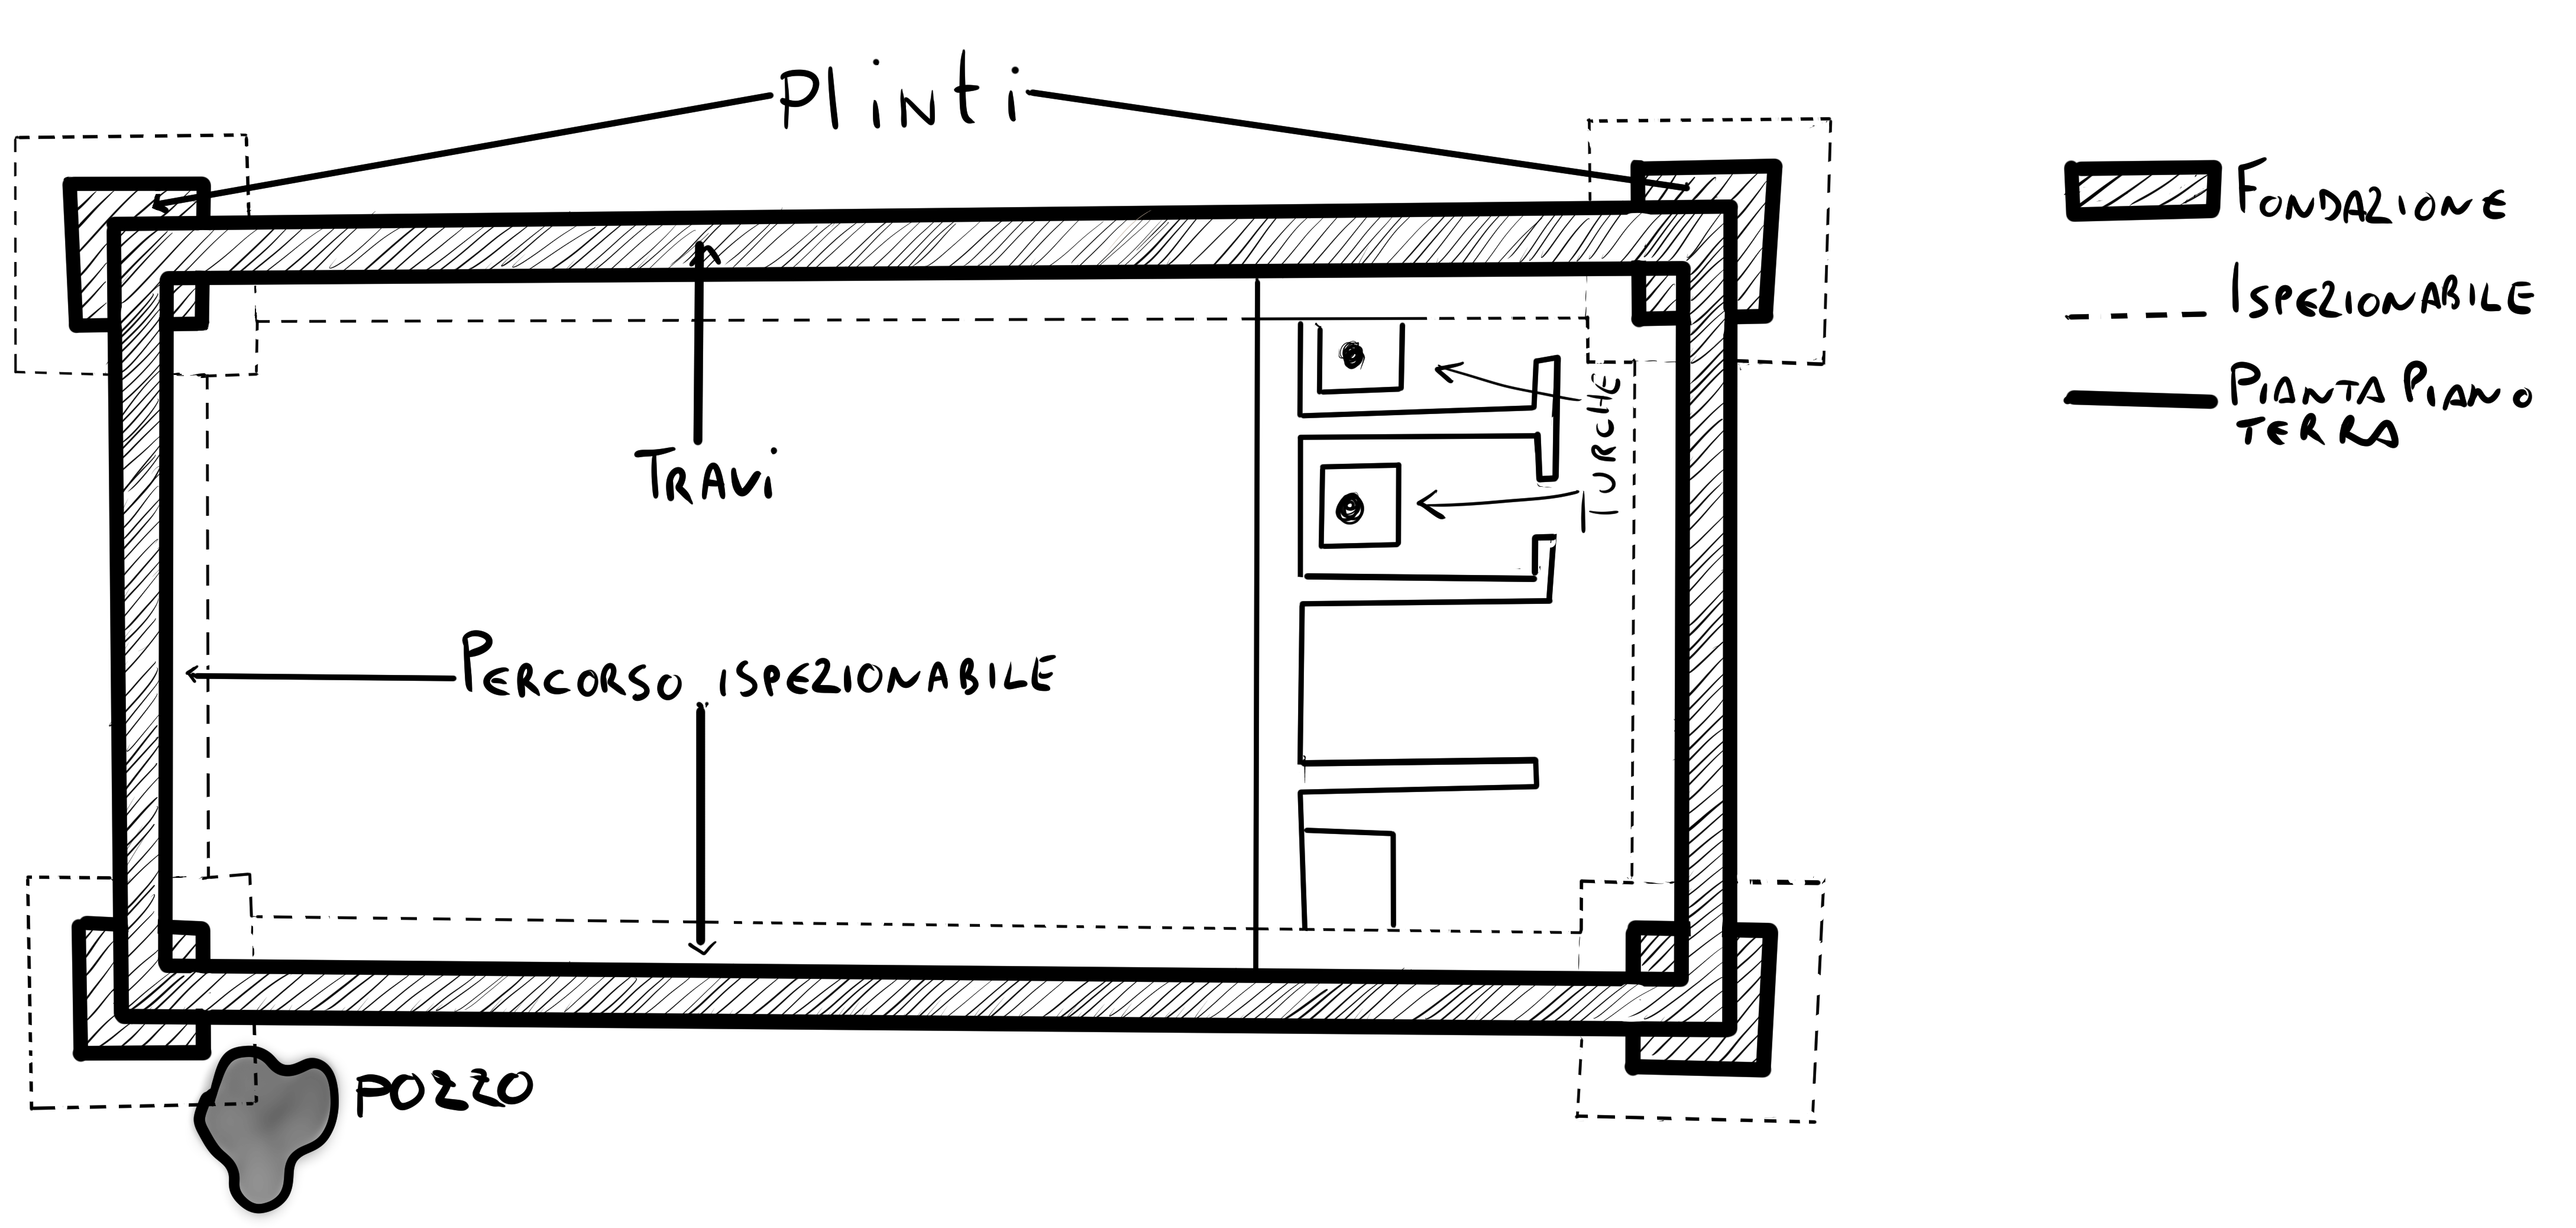
\includegraphics[width=0.9\linewidth]{fondazioni.png}
\end{center}

\par\medskip
«Sì, è un cavedio tecnico, un classico anni Settanta.»\\
«Laura, ma...»\\
«Cate, ora devi aiutarmi. Io entro nel pozzetto. Tu tieni la radio e rimani in ascolto.»\\
«Ok, Laura, io aspetto qui.»

\par\medskip
Laura indossa lo zaino e prova a calarsi, ma i piedi non toccano.  
Si lascia scivolare fino a terra, dove l’acqua le raggiunge quasi l’inguine.

\par\medskip
«Cavolo, è tutto allagato qui sotto.»\\
«Laura, aiuto! Qualcuno sta cercando di entrare!»

\chapter{Incontri nel buio}

«Qualcosa si sta avvicinando.» Giovanni \`e andato a prendere il peso da un chilogrammo per calare la corda a Luca; \`e compito del vagabondo tranquillizzare Luca:
«Stai calmo, non \`e niente. Forse un pesce.»\\
«Non \`e un pesce. Sento muovere l’acqua. Si sta avvicinando.»

\separatore
\par\medskip

«C’\`e qualcuno qui dentro? C’\`e qualcuno? C’\`e qualcuno?»
La porta del bagno trema sotto una forza esterna. Isl pomello della maniglia scatta avanti e indietro.\\
«Cate, mi senti? Chi sta cercando di entrare?»\\
«Non lo so! Ti prego, torna su!»\\
«Non riesco, Cate. Sono in un cunicolo stretto. Dammi un attimo.»\\
Caterina \`e chiusa nel gabinetto. Sotto di lei un pozzetto che conduce ad un condotto allagato. Alla porta qualcuno sta cercando di entrare, qualcuno di sconosciuto:
«Ecco, adesso apro» le annuncia da dietro la porta.
Poi si apre all’improvviso. Caterina resta immobile.
Osserva lo sconosciuto di fronte a lei.\\
«C’\`e qualcuno chiuso dentro?»\\
Caterina istintivamente si avvicina: «Tu non mi vedi?»\\
«Ah, ecco! Sentivo qualcuno. Stai bene? Ti hanno chiusa dentro le casalinghe, immagino.»

\par\medskip
«Cate, con chi stai parlando?»\\
«Puoi dirle che sono Giovanni e che non corri alcun pericolo?»\\
Da un po' ha dimenticato di sbattere le palpebre, ma ora lo fa. Poi un lieve sorriso, quasi incredulo:
«Mi dice di dirti che si chiama Giovanni, Laura, e che non corro alcun pericolo. Ha aperto lui la porta.»\\
«Bene, Cate. Se riesci, fatti condurre nella mensa. Io raggiungo Rocky da qui sotto e poi cerchiamo di recuperarlo.»

\par\medskip
Giovanni anticipa la richiesta, le prende un polso, delicatamente:
«Ho sentito, Cate. Forse siamo nello stesso guaio. Vieni, andiamo nella mensa. Ti guido io.»\\
La candela si \`e spenta, ma,  a questo punto della storia,  \`e chiaro che non un problema per lui.

\separatore

\par\medskip
Il vagabondo si sporge nel pozzo: «Ehi, ma chi sta parlando?»\\
Anche Rocky sente la voce di Laura e comincia ad abbaiare.

\par\medskip
«Chi c’\`e laggiù? Puoi aiutarci?»\\
Giovanni e Caterina hanno raggiunto la mensa. Il vagabondo \`e sdraiato e sta cercando di comunicare con Laura.\\
«Sì, credo possano aiutarci.»\\
«Giovanni, chi \`e questa ragazza con te?»\\
«Sì, si chiama Cate...  Caterina?»\\
«Cate, sei lassù?»\\
Luca riprende coraggio:
«Non \`e un pesce, \`e una ragazza con la torcia.»\\
«Ma chi c’\`e nel buco oltre Rocky?»\\
«\`E Luca, \`e un nostro amico. \`E finito dentro con Rocky.»

\par\medskip
La luce della torcia gli punta il viso. Fa una smorfia, ma la guarda: «Finalmente! Grazie, avevo paura di restare qui sotto.»\\
Rocky tenta di raggiungere la padrona. Ha la pettorina incastrata, non ci riesce, ma non importa: in un attimo Laura li ha raggiunti.
«Non so come siete finiti qui... ma conoscendo Rocky non mi stupisco. Tu stai bene?»\\
Laura prende Luca per la mano: «Sei incastrato?»\\
«Sì, ho la caviglia infilata da qualche parte, non riesco a sollevarmi.»\\
«Ho capito.» Alza il viso verso la luce del pozzo. «Cate, qui c’\`e un ragazzino incastrato insieme a Rocky.» Mentre parla si leva di nuovo lo zaino ed estrae rapidamente un piccolo paranco.
\par\medskip
Si arrampica fino a raggiungere l’uscita. «Prendi.» Trattiene il gancio e passa il corpo dello strumento a Caterina. «Tienilo.» Poi guarda verso Giovanni e fa un cenno di saluto, non corrisposto, per ovvi motivi, mentre il vagabondo la saluta con un cenno  del capo. Appoggia i palmi sul bordo e si tira su, lasciando una piccola pozzanghera. «Troviamo un punto dove appenderlo.»\\
Il vagabondo indica con il dito una putrella sopra le loro teste. Laura gli sorride. Lui prende una sedia, la sistema in prossimità dell’apertura, ci sale in piedi e guarda Caterina, che subito gli porge il paranco. Lui lo studia per pochi secondi, prende la cinghia di sospensione e la passa intorno alla putrella. Aggancia la cinghia: «Ci siamo.»\\
Laura ringrazia con un cenno e torna nel pozzo: «Pronti a tirare» avverte.

\par\medskip
\begin{center}
  
\includegraphics[width=0.7\linewidth]{paranco senza sfondo.png}
\end{center}

\par\medskip
Rocky abbaia. I movimenti della padrona lo eccitano, Luca ha smesso di lamentarsi. Laura scende con attenzione, cercando di non scivolare.\\
«Eccoci» li ha raggiunti. «Iniziamo con Rocky, visto che ti sta sopra!» Aggancia la pettorina. «Tirate piano, devo vedere dove si \`e incastrata.» Sfruttando il paranco sollevano il cane fino allo stop di Laura: «Ecco, un attimo e lo libero.»\\
«Rocky...» A Caterina sfugge una lacrima quando intravede le orecchie tese del disperso. Quanto sono lontani, adesso, il visto e i problemi ambientali.
Il vagabondo si sporge verso il pozzo per prenderlo e per un attimo la presa gli sfugge. Caterina si stringe involontariamente verso Giovanni, lui si gira verso di lei. «Scusami, ho preso paura.» Ma non serve giustificarsi. Sei umana, Caterina.\\
«\`E al sicuro» la informa il vagabondo. «Grazie; adesso lego il bimbo.»\\
«Non sono un bimbo, ho tredici anni.»\\
«Peccato, a quattordici ti sarebbe gi\`a cresciuta l’asola di aggancio!» Gli mostra il gancio. «Questo dove lo mettiamo?»\\
«Mi sento nel livello della cisterna.» Laura lo guarda interrogativa. Il riflesso della torcia le taglia il viso e sembra eccitare ancora di pi\`u la fantasia di Luca. «Sei sua figlia, vero? La figlia di Lord Richard?»\\
«Non so di cosa parli, ma se non vuoi restare qui sotto, chiudi la bocca e fai come ti dico.»
Gli fa scorrere la corda intorno al bacino, poi crea un’asola che dalla spalla sinistra passa sotto l’ascella destra.
Infine due asole fra le cosce.
«Sei pronto?»\\
«Sì, ma non sono un bimbo.»\\
«Ti ho chiesto solo se sei pronto.»\\
«Io sono nato pronto.» Laura stringe la corda; di nuovo ha l'impressione che tra le righe qualcosa le sfugga. «Sollevate.»


\chapter{La torta di mezzanotte}

Con un colpo secco e forza ben calibrata, ne sbatte uno contro lo spigolo del tavolo.  
Lo guarda colare dalla frattura.  
Nella mano sinistra regge un pacchetto di farina, che aggiunge al burro e all’uovo.

\par\medskip
«Ora mescoliamo per bene.»
\par
«Sì!»
\par\medskip
Valentina \`e entusiasta. Laura cucina raramente con lei dei dolci, mentre Alice sembra esperta.
\par\medskip
«Vuoi provare? Spingi bene in modo che si sciolga il burro.»\\
«Così?»\\
«Sì, cos\`i va bene. Vale, continua a mescolare.»
\par\medskip
Mentre Valentina mescola, Alice, a suo agio, sceglie la musica per accompagnare la preparazione.
\par\medskip
\begin{center}
  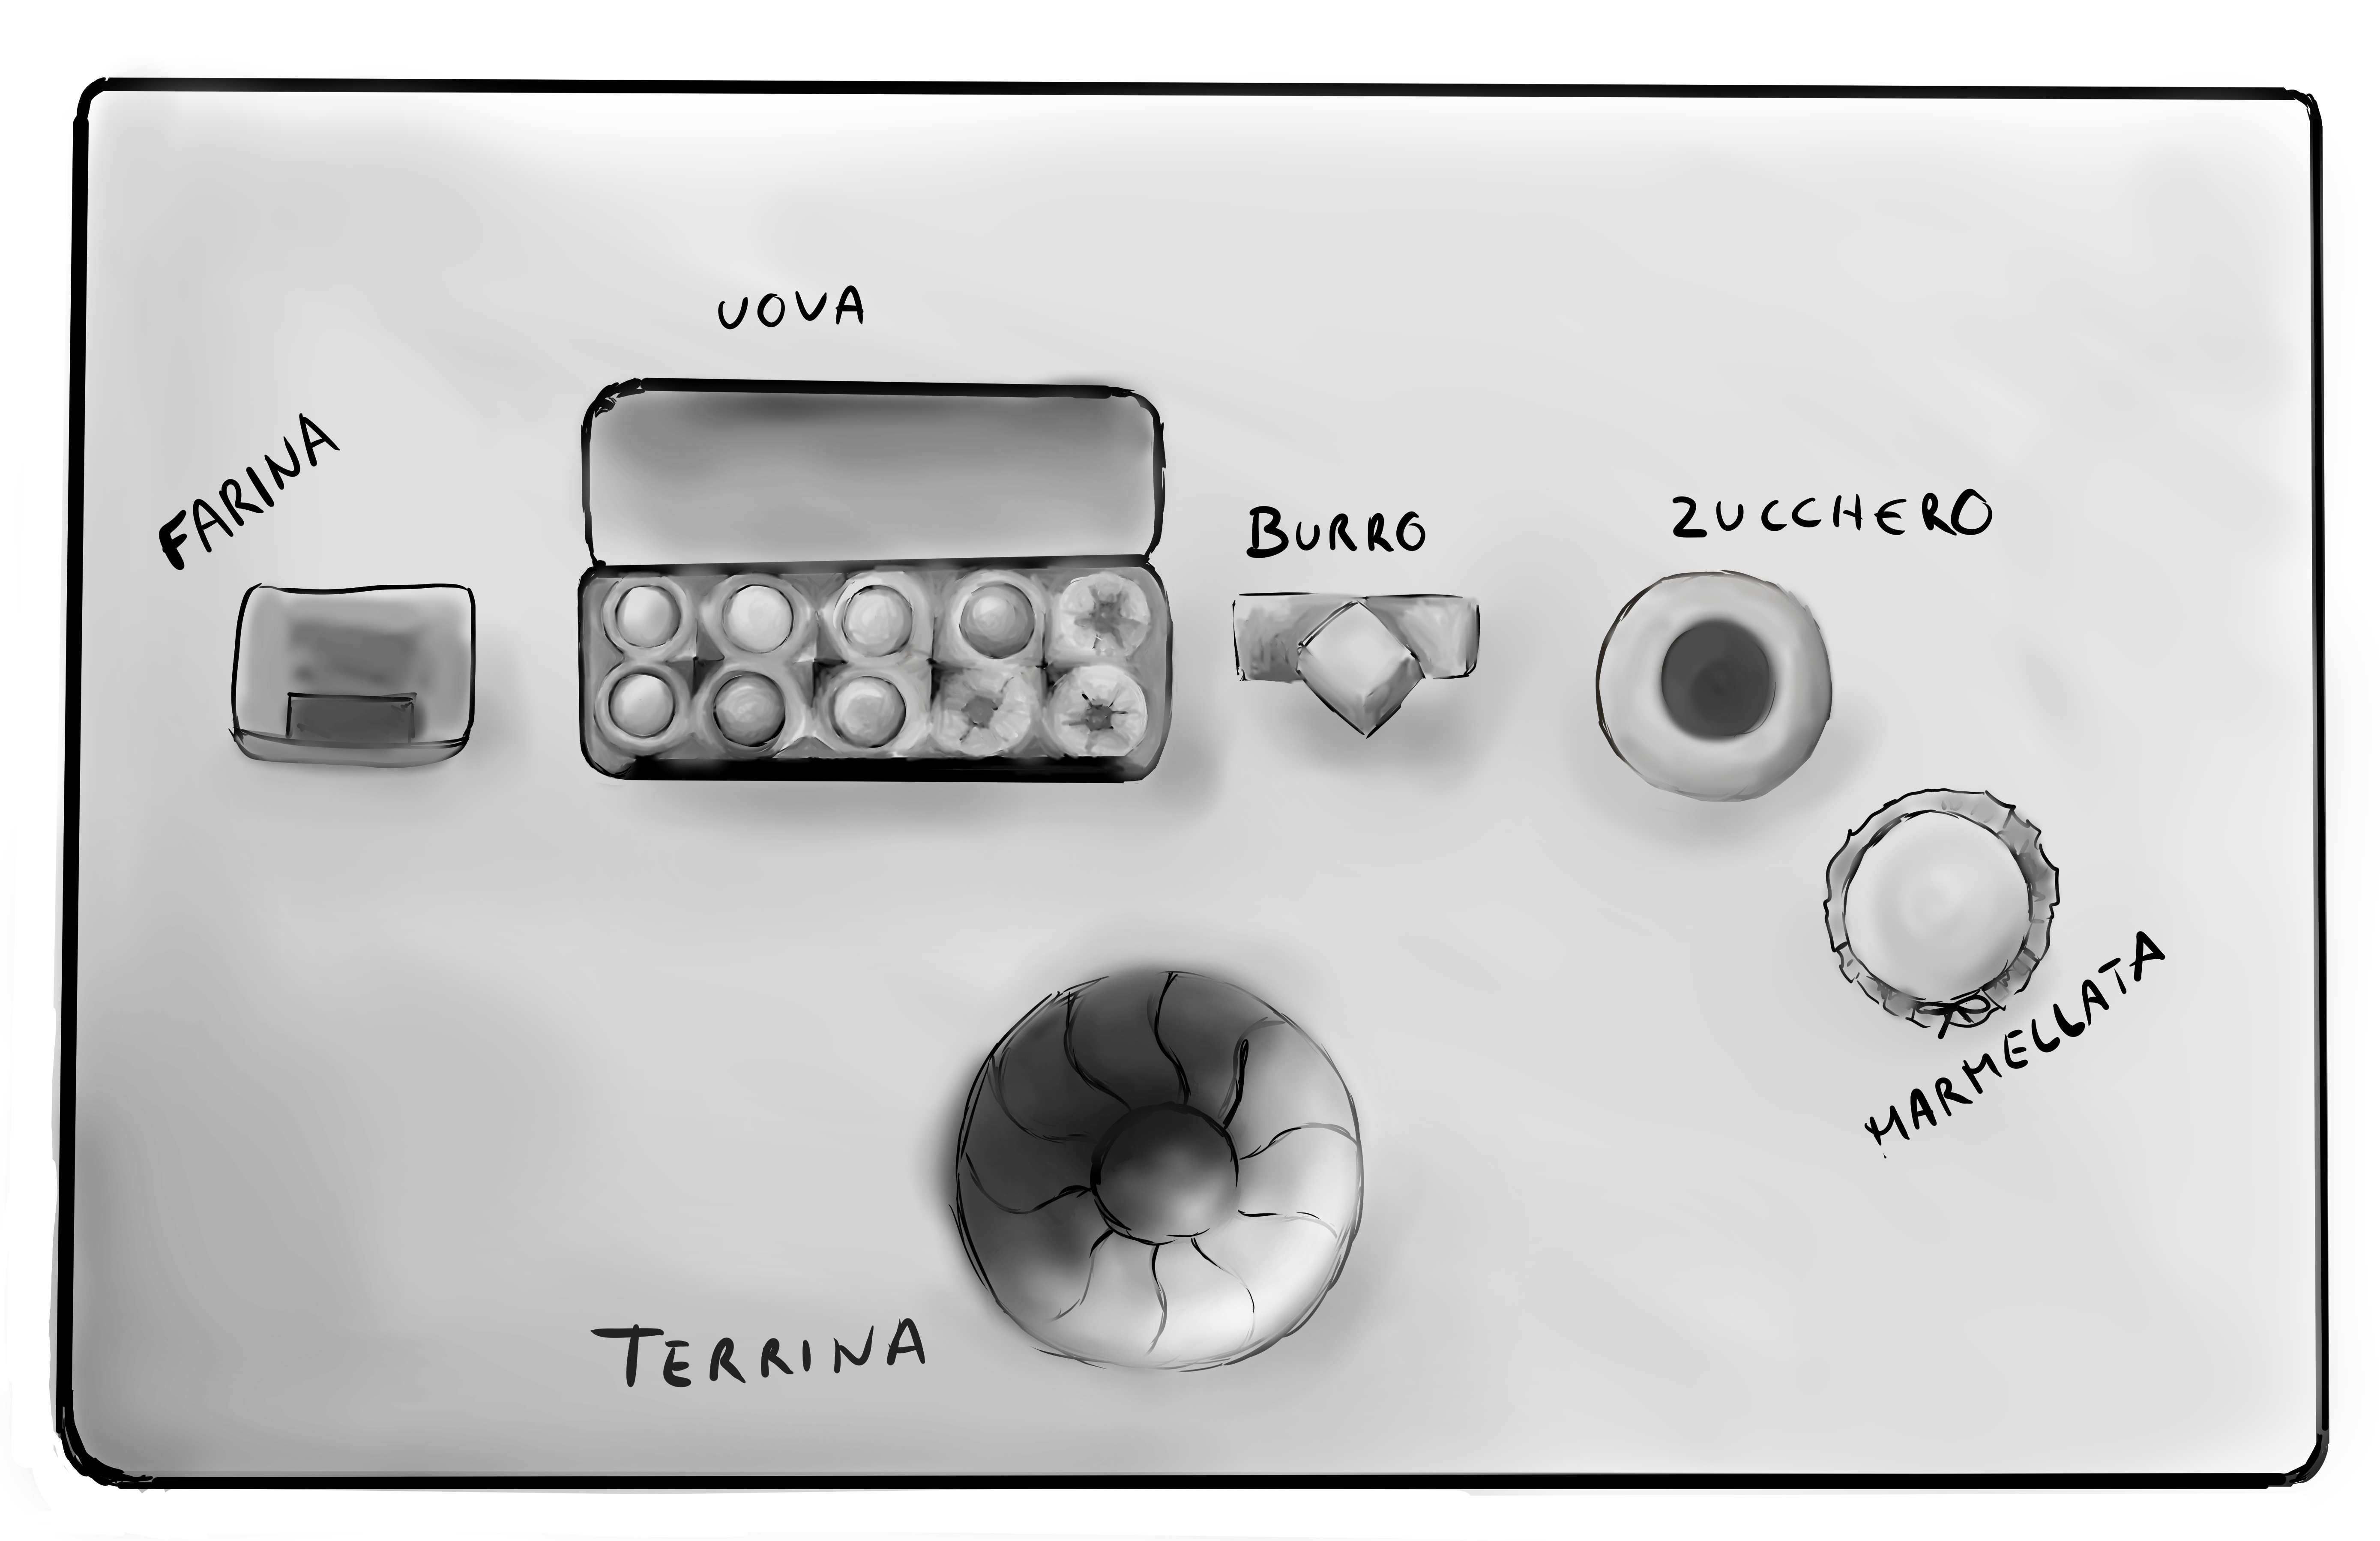
\includegraphics[width=0.8\linewidth]{crostata senza sfondo.png}
\end{center}

\par\medskip
«Ci siamo, Vale? Adesso in frigo per dieci minuti.»
\par\medskip
Si lavano le mani e insieme riprendono a guardare la foto dove Alice aveva interrotto.
\par\medskip
«Questa sei tu, piccolina?»\\
«Sì, ero appena nata. E quella \`e Laura, con la mamma. Il papà sta facendo la foto.»\\
«Ti mancano tanto?»\\
«Non li ricordo pi\`u tanto.»
\par\medskip
Il timer suona. Il burro si \`e raffreddato.  
E ora hanno un bel panetto di farina, uova, zucchero e burro,
 da trasformare in pasta frolla.
\par\medskip
«E quello?»\\
«Con questo ci facciamo i bigoli. Non hai mai mangiato la crostata?»\\
«Ah, sì, adesso ho capito. Quelli sopra la marmellata?»\\
«Esatto.»\\
«Questa l’abbiamo preparata io e Laura.»\\
«Fantastico. Adesso la spalmiamo…»\\
«E intanto facciamo i bigoli.»\\
«Bravissima. Ora in forno trenta minuti.»\\
«Chissà che sorpresa quando tornano.»
\par\medskip
Vale va a prendere il suo futon in camera e lo porta in soggiorno.  
Si sdraiano insieme, lei e Alice.
\par\medskip
«Laura ti assomiglia molto da piccola.»\\
«E tu e Caterina vi assomigliate?»\\
«Non tanto», le dice, «io ho i capelli lisci.»\\
«Allora vi assomigliate solo quando avete i capelli bagnati.»\\
«\`E vero, almeno cos\`i ci assomigliamo.»\\
«Sei simpatica, Alice.»\\
«Anche tu sei simpatica.»
\par\medskip
Valentina si addormenta, mentre Alice aspetta perch\'e vuole controllare la cottura.
Sono ormai le ventitré. Alle ventiquattro sarà troppo tardi per la revisione del visto,
ma di questo Alice non sa nulla.

Le parole della sua canzone le risuonano nella mente. Hanno cristallizzato il suo dolore,
ma il profumo della crostata la riporta alla vita che non si cristallizza,
a una serata che potrebbe finire con un dolce da mangiare insieme.
Anche insieme a sua sorella.

\include{chapters/chapter13}
\chapter{Guerra di rete}

«Che schifo! Non mi leccare le orecchie.»

Rocky saluta entusiasta Valentina e Alice. \`E un cane di taglia media: se Laura non gi  limasse le unghie, le sue \textit{feste} lascierebbero dei ricordi netti sulla pelle. Per fortuna sono ben arrotondate, cos\`i, tranne qualche batterio, non lascia spiacevoli graffi sulle ragazzine.\\
Laura si spoglia della tuta, un po' calda per la stagione, e si infila una magliettina.
«Non era mai successo che si allontanasse da solo. Evidentemente deve aver subito il fascino della piccola vagabonda.»

«Già... Dai, \`e andata bene...»\\

Laura guarda l’amica: «Era un sospiro quello?»
Valentina si stropiccia gli occhi e prova ad abbracciare Rocky, che si sottrae agilmente e si accuccia ai piedi del futon.

\par\medskip
«Rocky! Cos'\`e successo? State bene? Ma \`e tutto baganto!»\\
«\`E una storia lunga, ma dopo ve la raccontiamo.»\\
«Sì, ragazze, adesso abbiamo bisogno che ci aiutate. Tra trenta minuti scade la possibilità di salvare il viaggio di Caterina. Quindi abbiamo bisogno di concetrazione assoluta.»\\

Alice guarda la sorella: «E se va male? Resti a casa?»\\
«Preferiresti?» le chiede. La osserva. Alice non risponde, ma \`e Laura a parlare: «Adesso non distraiamoci. Dobbiamo completare alcune... procedure informatiche. Quindi mi raccomando.»\\
Valentina le corre vicino: «Devi hackerare un sito, tata?»

\par\medskip
Alice spalanca gli occhi, gli hacker hanno perso il diritto di cronca prima che lei nascesse, per\`o dove conta se ne parla ancora, e una ragazza intelligente non si lascia sfuggire certi dettagli: «Cosa? Sei anche un'hacker? Ma \`e fantastico!»\\
Laura non si sforza di negare, ma una precisazione \`e dovuta:
«Vista la rete in cui devo entrare diciamo che non \`e proprio hacking, \`e pi\`u archeologia digitale... Ragazze, \`e meglio se di queste cose non ne parliamo con nessuno, ok?»\\
«Vogliamo solo capire perch\'e mi hanno negato il visto» completa Caterina.\\
«Cos’\`e il visto? A proposito, ma ci stiamo dimenticando della...» A Valentina manca un grosso pezzo della storia, per\`o ha chiara in mente un'altra faccenda, peccato che il suo entusiasmo venga fermato dalla \textit{consorella minore} che la pizzica, le strizza l’occhio e si avvicina al suo orecchio: «Dai, non dire niente che facciamo una sorpresa alla fine.»\\
Valentina ricambia il gesto confidenziale: «Ok», le conferma e sigilla il patto con un pizzicotto meno trattenuto che la fa sobbalzare.

\par\medskip
«Va bene. Prepariamo gli strumenti.» Laura ha poco tempo e molto bisogno di concentrazione.\\
«Ma da quando sei una hacker?» le chiede Alice. Si sposta vicino a lei. «Questo allora \`e un sistema operativo per voi... hacker?»\\
Laura la guarda, le sorride. Il tempo stringe. «Sì, \`e un sistema dedicato...»\\
«Mi fai vedere come funziona?» Alice guarda la sorella. La contrazione delle labbra di Caterina esprime il suo rimprovero, ma poi il rimprovero diventa verbale: «Alice, abbiamo davvero poco tempo.»\\
«Ho fame, mangiamo un dolce?» Valentina torna alla carica. Nonostante la raccomandazione della consorella minore, il pensiero della crostata le stimola l’appetito.\\
Laura chiude gli occhi, prende un respiro. Conta sottovoce fino a cinque, solleva le dita dalla tastiera: «Avrei bisogno che per dieci minuti steste in riga, brave e ordinate, ok? Poi rispondo a tutte.»\\
Il sorriso di Valentina illumina la stanza pi\`u del monitor di Laura: «Giochiamo all’intrusione? Ti prego, Tata, fai le vocine.»\\
«Non mi hai capito, Valentina», la voce \`e ferma e leggermente bassa, «ho detto che abbiamo i minuti contati, non abbiamo tempo di giocare.» Guarda una per una le tre ragazze: «Per questo abbiamo bisogno di... pianificare perfettamente l’operazione. Mappare l’infrastruttura per identificare i punti deboli e sondare il terreno con una perlustrazione a bassa intensità.»\\
A quanto pare la missione \`e iniziata e il capitano della squadra \`e indiscutibilmente Laura. I comandi diventano armi, il terminale una mappa, le righe di codice corridoi da attraversare. Ma dietro il gioco la partita \`e vera: non contro qualcuno, ma contro il tempo.
\par\medskip
\begin{center}
  \includegraphics[width=0.7\linewidth]{piantina casa laura senza sfondo.png}
\end{center}

«Sì!» la incita Valentina. Alice si avvicina alla sorella e segue la scena con lei.

\par\medskip
Laura esegue una scansione delle porte del vecchio sistema informatico della polizia locale.

\par\medskip
«Bene. Procediamo con uno \textit{script} veloce. Prendiamo il binocolo tattico e osserviamo le linee nemiche...»

\par\medskip
«Vai Laura!»

\par\medskip
«Fuoco!»

\par\medskip
Laura \`e decisa e schiaccia il tasto INVIO con determinazione ma senza forza. La sensibilità \`e importante. Un comando non deve partire per sbaglio.
\par\medskip
\begin{terminalbox}
laura@dpl:~$ nmap -sS -p21,80 35.228.xxx.xxx
Starting Nmap 7.80 ( https://nmap.org ) at 2041-10-03 23:32 CEST
Nmap scan report for 35.228.xxx.xxx
Host is up (0.088s latency).

PORT   STATE SERVICE
21/tcp open  ftp
80/tcp open  http

laura@dpl:~$
\end{terminalbox}

\par\medskip
«Bene. Abbiamo trovato. Ci sono due porte aperte. Procediamo.»

\par\medskip
Alice sta stringendo la mano a Caterina. Chissà se se ne \`e accorta o se lo ha fatto automaticamente. Ma mentre racconto, Laura \`e gi\`a pronta per la sua prossima mossa.

\par\medskip
«Prepariamo il grimaldello... questo no, troppo invadente... questo no...», Laura verifica diversi comandi al terminale. «Ah! Eccolo, il mio preferito, si insinua come un'\textit{Idra} e  apre le porte ordinarie senza farsi sentire.»\\

\par\medskip
«Cosa fai, Tata?»

\par\medskip
«Abbiamo trovato un varco nella loro recinzione, una porta mal sorvegliata e adesso proviamo a vedere che serratura ha.»

\par\medskip
Il silenzio si potrebbe pesare. Anche Rocky \`e immobile, ma forse gi\`a dorme. Alice fissa Laura che intanto ha ottenuto qualche nuova informazione:\\
\begin{terminalbox}
laura@dpl:~$ hydra -l ftpuser -P password.txt ftp://35.228.xxx.xxx
Hydra v9.2 starting at 2041-10-03 23:34:11

[DATA] max 16 tasks per 1 server
[DATA] 102 login tries: 1 user / 102 passwords
[DATA] attacking ftp://35.228.xxx.xxx:21/

[21][ftp] host: 35.228.xxx.xxx   login: ftpuser   password: ftppass

1 of 1 target successfully completed.
1 valid password found.

Hydra finished at 2041-10-03 23:34:19
laura@dpl:~$
\end{terminalbox}

«Davvero? Queste credenziali cancellano i miei sensi di colpa. La polizia locale se l’\`e cercata.»\\
Caterina sgrana gli occhi e apre leggermente le labbra. Ma Laura le strizza l’occhio e le sussurra:
«\`E un gioco, Cate. Non faremo danni.»

\separatore

\par\medskip
La sala di controllo della polizia  \`e tranquilla. \`E quasi mezzanotte. Gli agenti sono al termine del loro turno. Ore passate a sorvegliare sistemi informatici diventati obsoleti, ma ancora funzionanti. Sottobosco digitale, pullulante di attività tutto sommato innoqua e di scarsa rilevanza.\\
Un agente nota un cursore cambiare colore e spostarsi a destra lasciando una scia di lettere alla sua sinistra. Si avvicina, osserva il monitor:
«Attacco BruteForce sul server 35.228...»\\
Il capitano sta prendendo un caff\`e. Lo appoggia, si avvicina all’agente: «Fa’ vedere. \`E una cosa seria?»\\
Sbadiglia: «Identificate l’IP e vediamo da dove arriva. Sarà ancora uno di quei retrò.»


\chapter{L’eterno mutamento}

«A cosa stai pensando?»\\
«Niente. Guardavo le stelle.»\\
«Che costellazione vedi, Giovanni?»\\
«Non le riconosco pi\`u. Pensi che i cieli stiano cambiando?»





\par\medskip
Gli occhi di Giovanni sono chiusi e la testa \`e rivolta al cielo.
Il Grande Carro \`e quasi sdraiato sotto la Stella Polare,
lui invece \`e sdraiato sulla rete del vagabondo.
Fa caldo, ma hanno acceso un fuoco dentro uno dei bidoni.

\par\medskip
«Quando mai sono rimasti uguali a se stessi?»\\
«E ora? In cosa muteranno?»\\
«Te lo chiedi perch\'e il mondo \`e tornato a interessarti?
Vuoi capire se tu puoi averci ancora a che fare?»\\
«Quante domande fai per essere uno che non ama parlare?
Non lo so. \`E che mi chiedo se questa volta il mondo sia cambiato pi\`u del solito.
\`E lo stesso cambiamento o \`e un cambiamento diverso?»\\
«Tu cosa pensi? So che se me lo chiedi...»\\
«No, non ho gi\`a una mia idea. Ho rinunciato alle idee.
Le idee mutano in fretta. \`E inutile possederle.
Chiamiamo idea un processo mentale...»\\
«Già, ma dimmi, Giovanni, quale mutamento delle tue abitudini ti ha cos\`i turbato?
Senti bisogno di una \emph{cate...}chesi?»\\
«Lascia perdere. Quando la vista ha iniziato a calarmi \`e stato l’olfatto il senso che ho sviluppato maggiormente.
Un odore pu\`o parlarmi per ore e io posso stare ore ad ascoltarlo.»

\par\medskip
«Ad ascoltarla, vuoi dire. Io comunque odorerei volentieri una bella torta.
Il dolce \`e l’unica cosa che mancava stasera.»

\par\medskip
La Stella Polare \`e rimasta ferma, mentre le sette stelle del Carro si trovano in una posizione diversa ora.
La loro distanza relativa \`e la stessa: nel complesso l’intera costellazione non ha cambiato forma.
\`E stata una trasformazione isometrica, una rotazione delle stelle attorno alla Polare.
Per questo lei \`e rimasta ferma.

\par\medskip
«Comunque io credo che il mondo, la biosfera, Gaia, gli d\`ei, il Tao, tutto si trasformi,
ma che qualcosa rimanga sempre tale e quale.
E quel qualcosa sai cos’\`e?»

\par\medskip
Giovanni ascolta l’amico e si gira verso di lui.
Questa piega della conversazione deve averlo incuriosito.

\par\medskip
«Il tempo?»

\par\medskip
\begin{center}
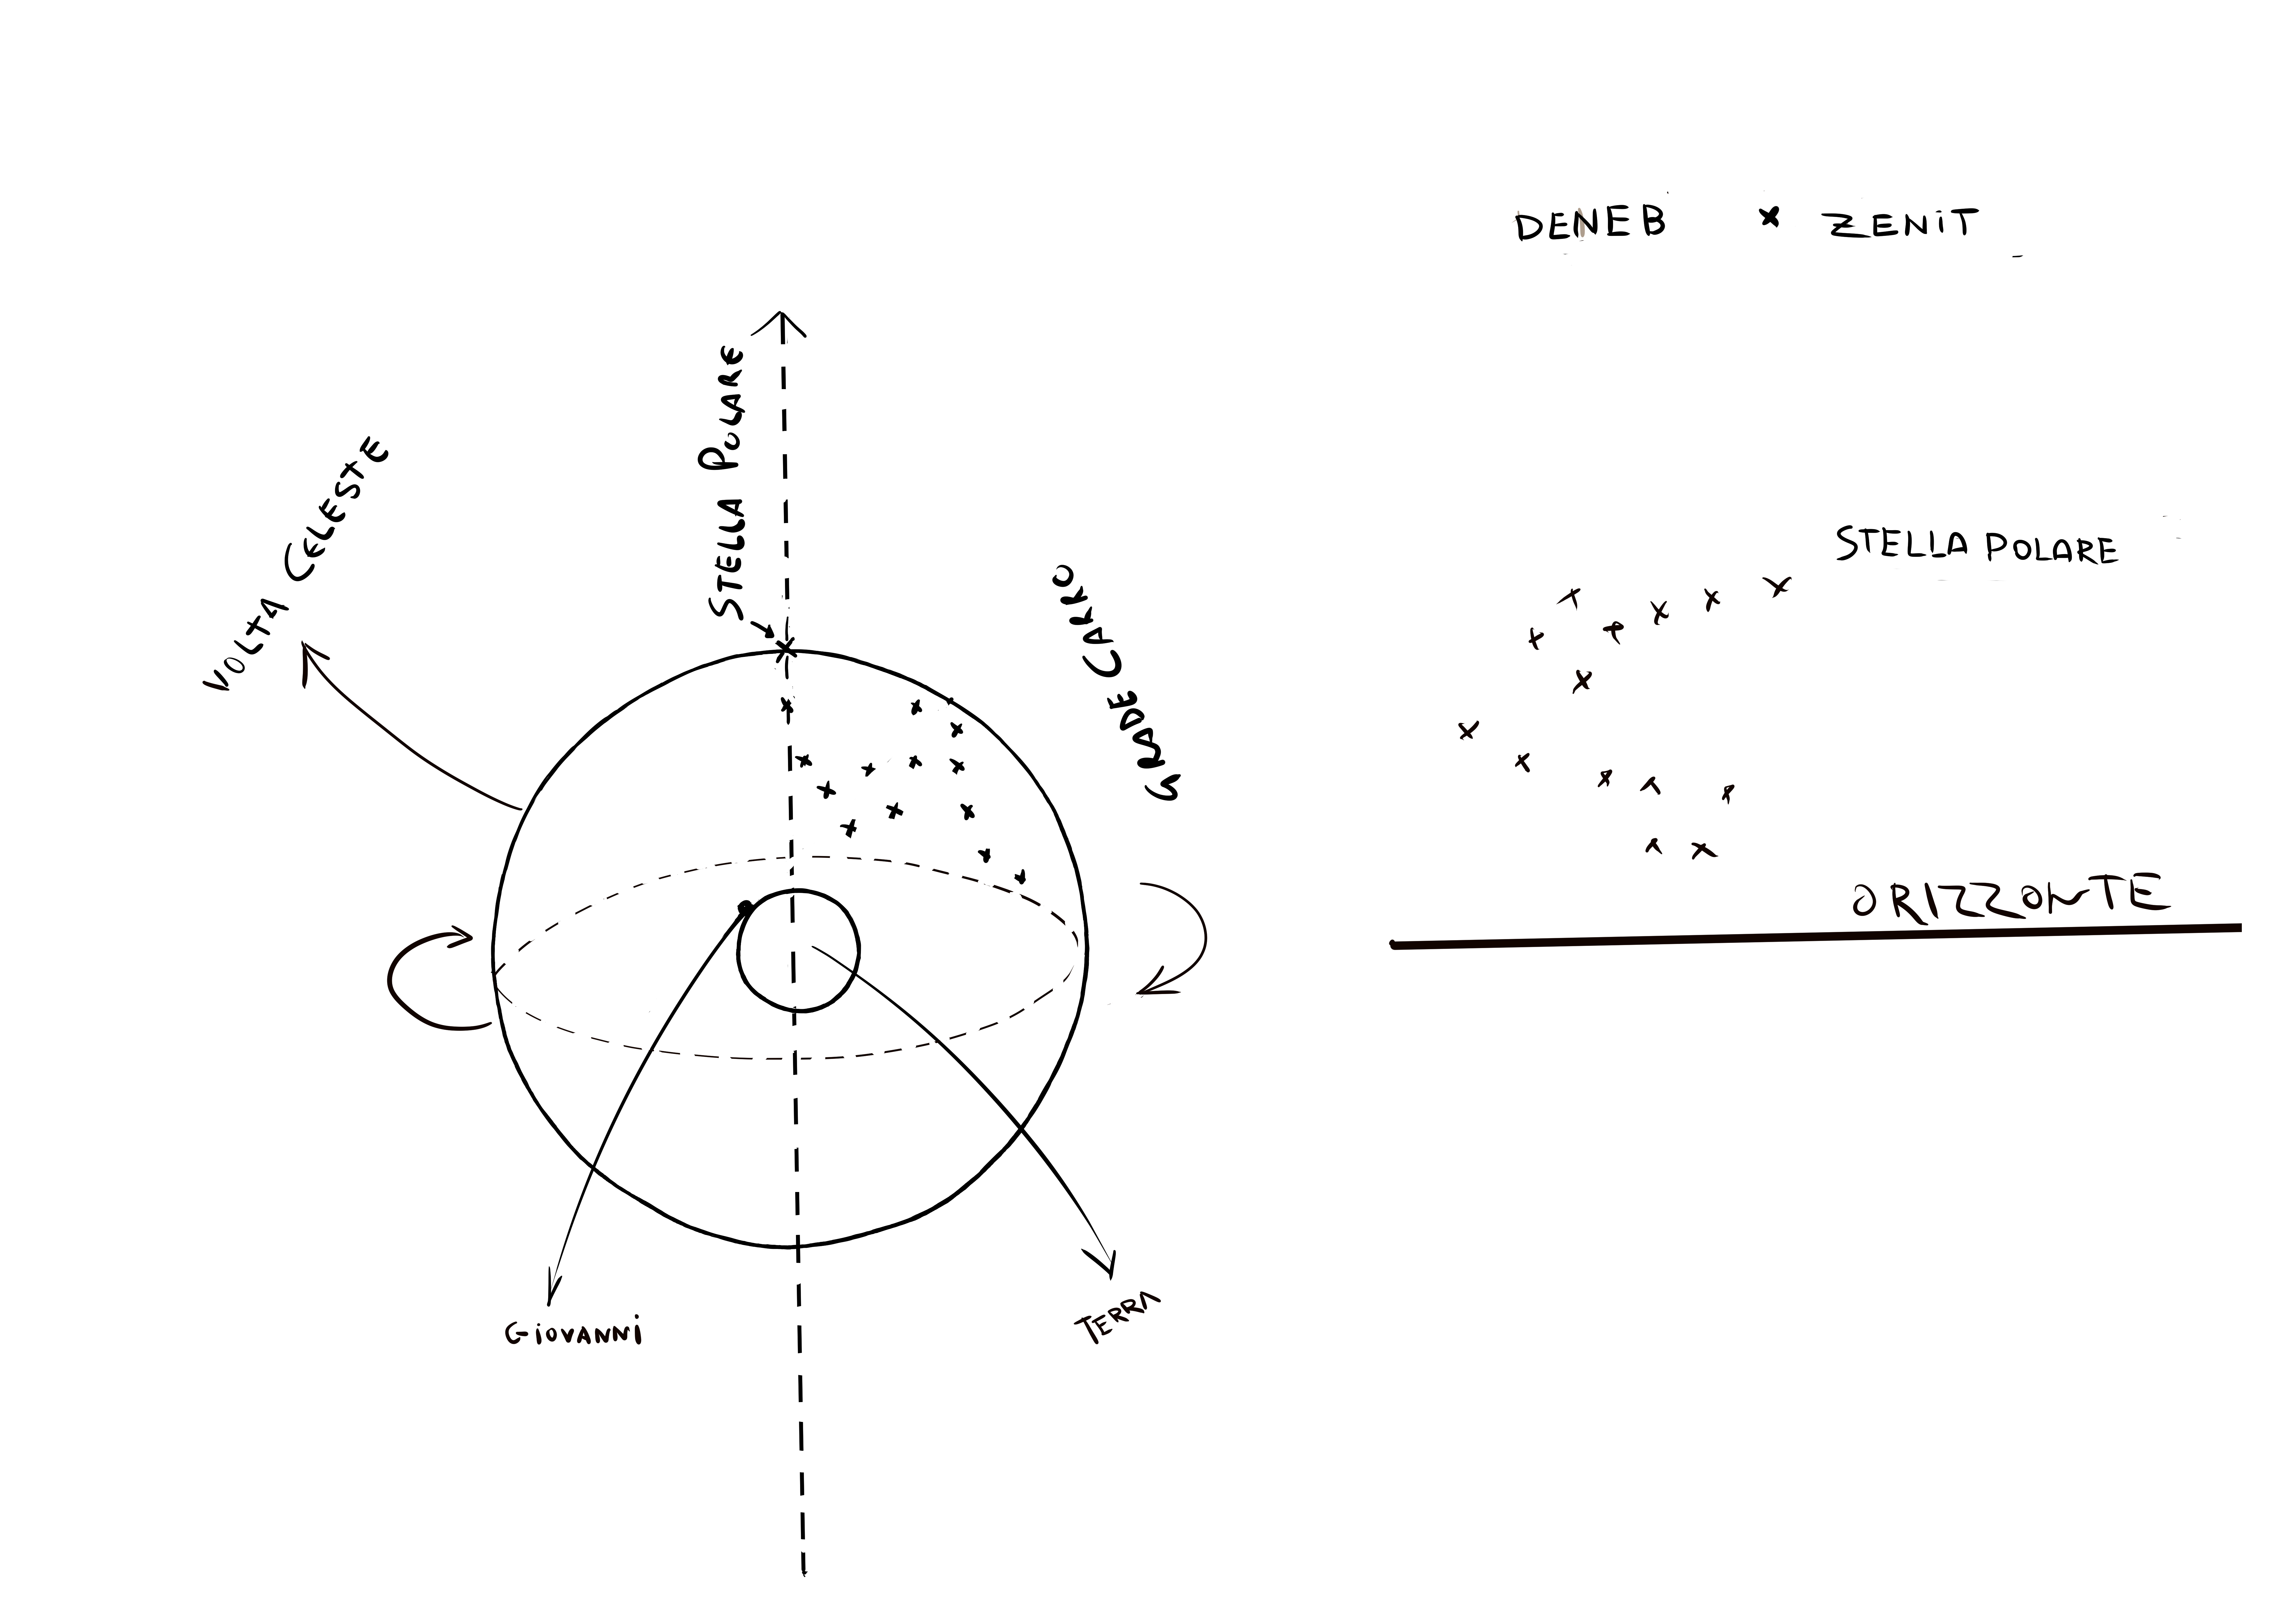
\includegraphics[width=1.0\linewidth]{planisfero senza sfondo.png}
\end{center}

\chapter{Nel mirino della Polizia}

Alice stringe la mano di Caterina. Chissà se tra sé sta ancora canticchiando i versi  che le ha scritto solo sette ore fa.\\
Valentina non riesce a stare ferma e saltella sul cuscino con un'emozione esplosiva reattiva ai comandi parabellici impartiti dalla sorella.


\par\medskip
«Bene, cambiamo arma. Via il grimaldello e attiviamo un fucile di precisione. Possiamo sparare usando le informazioni ottenute: sbagliare non \`e un'opzione in questa missione.»

\par\medskip
Preme INVIO.
\par\medskip
\begin{terminalbox}
laura@dpl:~ ftp 35.228.xxx.xxx
Connected to 35.228.xxx.xxx.
220 (vsFTPd 3.0.3)
Name (35.228.xxx.xxx:laura): ftpuser
331 Please specify the password.
Password:
230 Login successful.
Remote system type is UNIX.
Using binary mode to transfer files.
ftp>
\end{terminalbox}

\par\medskip
«Accesso autorizzato. I cancelli sono aperti, iniziamo l'esplorazione. Massima attenzione... tutte! Abbiamo trovato un fascicolo. C'\`e qualcosa.»\\
Valentina si agita vicino alla sorella: «Tata!»\\
«Che succede, soldato?»\\
«Niente, niente, continua.»\\
«Ti scappa la pipì, soldato?»\\
«No, no, la tengo!»\\
«Brava! Adesso vediamo un po’ cosa c’\`e scritto qui dentro:»

\begin{terminalbox}
ftp> less ftpuser/readme.txt

LEGACY DATA INDEX
Last update: 2041-09-28
Maintainer: local-admin

The following paths are still used by legacy services.
Do not rename or move files without updating the corresponding jobs.

Main files:

  /data/in/cassa.csv              foreign accounts import
  /data/war/bann.txt              banned subjects list
  /etc/conf/mys.txt               local security configuration
  /var/lib/mysql-files/flag.txt   registered organizations export
  /data/cnt/crb.csv               contact records backup

Notes:
- Files under /data/in/ are read by the nightly import task.
- Files under /data/war/ are checked before access validation.
- /etc/conf/mys.txt is required by the old MySQL connector.
- /var/lib/mysql-files/ is exposed only to the database service.
- /data/cnt/ contains temporary contact exports.

ftp>
\end{terminalbox}

\pagebreak
«Gli hai tracciati?»\\
«Sì. Il collegamento \`e da una cittadina in Polonia, ma \`e sicuramente una falsa uscita della VPN.»\\
«Analizza le impronte. Vediamo da dove arriva davvero.»\\
«Sì, lo sto facendo. Anche se tra poco finirei il turno, forse...» non finisce la frase, il suo capitano \`e di un altro avviso.\\
«Coraggio, quest'anno avremo il premio di produzione. La faremo vedere noi a quegli appendi multe del reparto droni.»\\
«Ok capo! L’hai detto. Premio di produzione! Ecco, ci sono quasi. Ho la time zone. E non \`e quella polacca.»
\par\medskip
«Cos'hai trovato Laura?» Caterina prova a stare al gioco, ma la voce tradisce l'emozione, ha paura di non farcela, di non riuscire a partire, anche se forse ora \`e attratta anche  da quello che potrebbe trovare restando.\\
Laura mantiene la calma, non pu\`o uscire ora dal suo ruolo: «Soldato, non sei autorizzata a fare domande. Mantieni il bersaglio sotto tiro. Ho individuato la directory e il file che stavamo cercando. Lì ci dovrebbero essere  i dati freschi per il TECS, il database principale del Dipartimento per la Sicurezza Nazionale degli Stati Uniti. Aprirlo \`e il nostro obiettivo. Deve essere un'operazione silenziosa.»\\
«Ho pipì, puoi aspettare?»
Laura guarda Valentina fissa negli occhi: «Operazione autorizzata, soldato. Hai 33 secondi da ora.»\\
Il bagno non \`e lontano dal soggiorno e in un attimo Valentina \`e di ritorno.

\par\medskip
«Acqua?»\\
«Tirata.»\\
«Mani?»\\
Valentina torna in bagno e dopo pochi secondi \`e a rapporto:
«Lavate.»\\
«Bene, allora possiamo procedere.»\\
«Che succede, Laura? Dici che ce la facciamo?»\\
«Credo di sì. Se nessuno si mette a rompere le uova nel paniere.»

\par\medskip
\begin{center}
  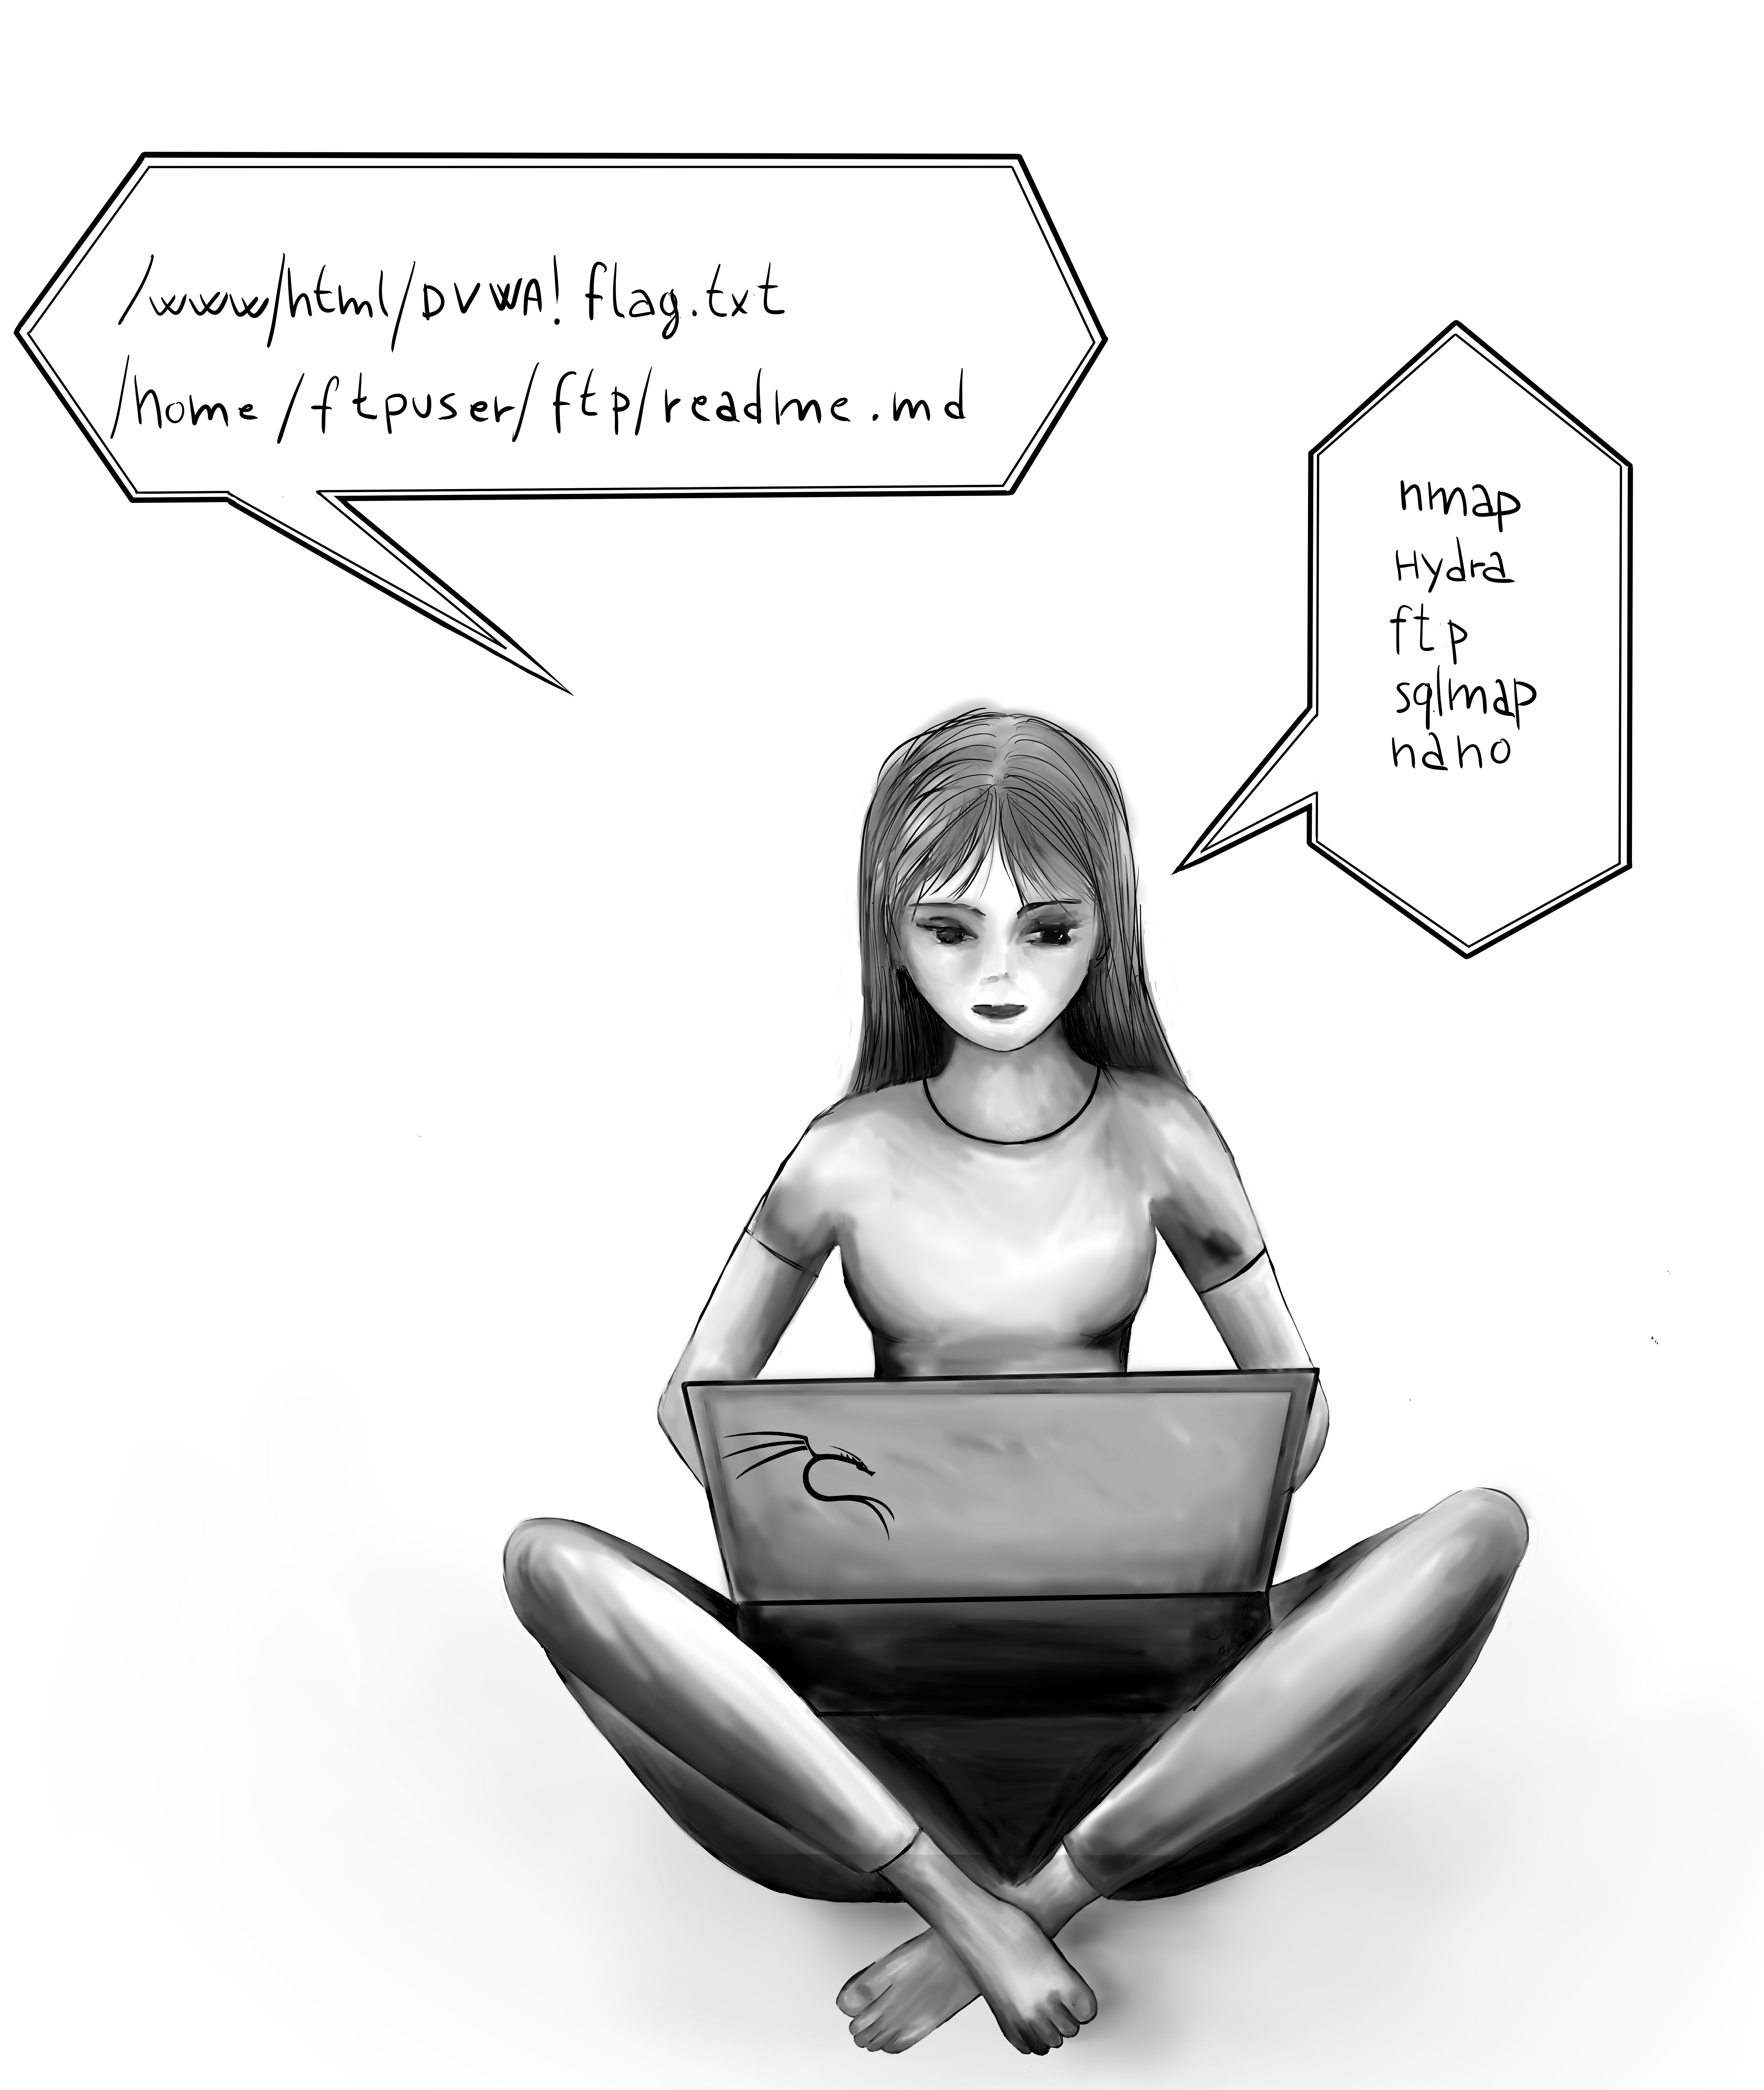
\includegraphics[width=0.55\linewidth]{laura pc senza sfondo.png}
\end{center}

\separatore

\par\medskip
«Capo, la combinazione di fingerprint corrisponde ad un agente ostile che risulta gi\`a profilato. Il server da cui sta uscendo \`e gi\`a compromesso. Se mi dai pochi minuti, forse lo vedremo in diretta dalla sua webcam.»\\
La polizia "ha fatto i compiti" o forse Laura ha fatto il passo pi\`u lungo della gamba.

\separatore
\par\medskip
«Tento l'accesso, silenzio assoluto:»

\begin{terminalbox}
laura@dpl:~$ sqlmap --flush-session
-u "http://35.228.xxx.xxx/DVWA/vulnerabilities/sqli/?id=1&Submit=Submit"
--cookie="PHPSESSID=********; security=low"
--batch --no-cast
--file-read="/var/lib/mysql-files/flag.txt"

[INFO] GET parameter 'id' appears to be injectable
[INFO] GET parameter 'id' is vulnerable
[INFO] the back-end DBMS is MySQL
[INFO] fetching file: '/var/lib/mysql-files/flag.txt'
[INFO] local copy and remote file have the same size: 627 B

files saved to:
[*] /home/laura/.local/share/sqlmap/output/35.228.xxx.xxx/files/_var_lib_mysql-files_flag.txt

laura@dpl:~$
\end{terminalbox}


\par\medskip
«Ottimo, vediamo cosa c’hanno scritto dentro.»

\begin{terminalbox}
1. Clara Whitmore | Green Force | Surveillance: Yes
2. Thomas Hale | NO Artificial Intelligence | Surveillance: No
3. Eleanor Price | No Vax Enthusiasts | Surveillance: Yes
4. Margaret Collins | Animal Rights Advocates | Surveillance: No
5. Daniel Mercer | Digital Freedom Fighters | Surveillance: Yes
6. Rebecca Stone | Climate Action Now | Surveillance: No
7. Hannah Reed | Anti-Surveillance League | Surveillance: Yes
8. Arthur Bennett | Renewable Future Coalition | Surveillance: No
9. Julia Hart | Cyber Privacy Watch | Surveillance: Yes
10. Samuel Grant | Human Rights Front | Surveillance: No
11. Caterina xxx | Green Force | Surveillance: Yes
\end{terminalbox}

«Cos'hai trovato Laura?»\\
«Il tuo nome.»\\
«Ma dice \texttt{sorveglianza: sì}! Cosa significa?»\\
«Esattamente non lo sappiamo, ma questo file probabilmente raggiungerà il DHS tra meno di cinque minuti. Se mi autorizzi, io cambierei quel \texttt{sì} in un \texttt{no}.»\\
«Il DHS? Cosa sarebbe, Laura?»\\
«Cate, il DHS \`e il Dipartimento per la Sicurezza Interna degli Stati Uniti. Raccolgono tutti i dati possibili, anche le tracce disperse dai vecchi sistemi locali, come quello che ti deve aver segnalato dopo il vostro» si ferma, tentenna un attimo, «arresto?» A Laura scappa una risatina. «Probabilmente nessuno ce l’ha con te, ma questa informazione esiste e alla SAGA-M potrebbe non piacere. Dobbiamo correggerla prima di mezzanotte, se vogliamo dare una chance al tuo visto.»\\
«Ho capito. Va bene, spero tu non ti metta nei guai per me.»\\
\separatore
\par\medskip
«Ho trovato la webcam. Il flusso \`e accessibile.»\\
«E la spia?»\\
«Firmware, passa dallo stesso controller. Posso escluderla prima di avviare il video.»\\
«Fallo. Vediamo cosa c’\`e dall’altra parte.»\\

\separatore
\begin{terminalbox}
 systemd[1]: Started Network Manager Dispatcher Service.
 NetworkManager[742]: connectivity state changed: FULL
 sshd[2184]: session opened for user service
 cam-bridge[2191]: device /dev/video2 requested
 cam-bridge[2191]: video stream initialized
  webcam-trap[2196]: LED_OFF requested - camera decoy triggered
\end{terminalbox}
Una riga del registro attira l'attenzione di Laura.
Si fa seria per un attimo, ma non dice nulla. Apre un secondo terminale e verifica i dispositivi connessi.
Un sorriso, un comando. Invio.
\separatore

Sul monitor della polizia si compone lentamente una figura, byte dopo byte.\\
«Ci siamo! Sembrano essere pi\`u di una persona!»\\
L’immagine mostra due sagome, forse due hacker mascherati. Indossano vestiti degli stessi colori. La definizione non \`e ancora buona, ma ogni pochi secondi emergono nuovi dettagli. I due hanno camicie uguali, quasi divise.\\
«Sono due. Direi agenti, ma...» L’agente si blocca. «Accidenti. Addio premio di produzione. Io chiudo, capo.»\\

\separatore
\par\medskip
«Bene, e ora il colpo finale. Mettiamo via le armi da fuoco e passiamo all’arma bianca.»

\par\medskip
Laura apre il file in modalità di modifica e cambia \textbf{Yes} in \textbf{No}:\\
«Ecco fatto. Così non risulti pi\`u in sorveglianza per quella manifestazione.»\\
«Che manifestazione, Cate?»\\
«Niente, Alice, una conferenza sit-in sull’ambiente che non sembra essere gradita agli “amici” di Mark.»\\
Laura guarda Caterina, lei abbassa lo sguardo. \`E stata cattiva... e lo sa.

\par\medskip
Mancano 40 secondi alle 24:00:00 NTP. Forse \`e meglio che Laura completi.

\par\medskip
«Caricamento tattico e via: il payload \`e in volo. File trasferito.»\\
«Ce l’hai fatta?»\\
«No, ce l’abbiamo fatta», risponde Laura.\\
Cate abbraccia l’amica. Alice apre le braccia, poi anche Valentina. Ora sono tutte abbracciate. Chissà se si ricordano della torta.


\chapter{Ombre sulla vittoria}

Sono le sette del mattino, il sole è già sorto e le casalinghe hanno iniziato le prime pulizie.
Sono arrivate delle artiste e nei paraggi stanno preparando gli intonaci per le loro \emph{street art}.
Giovanni ha dormito vicino al vagabondo, non dentro, fuori, su una rete metallica arrugginita.
Ippa è sotto, esce e punta i rovi di cinta.
Le orecchie sono tese.
Qualcuno sta penetrando nel convitto.

\par\medskip
«Saranno le artiste che cercano un posto esotico per le loro creazioni.
Dai, Ippa, abbaia, così scappano e non vengono a romperci l’anima.»

\par\medskip
I latrati non vanno a vuoto e ricevono in risposta un altro latrato.
Giovanni sorride.
Dal tunnel di rovi escono Laura, Valentina, Alice, Rocky e Caterina, che porta una torta.

\par\medskip
«Buongiorno, siamo passati a salutarvi.»\
«Ragazze, buongiorno. Vedo che non venite a mani vuote.»

\par\medskip
Giovanni si alza e insieme a Ippa si avvicina al grupo.

\par\medskip
«Abbiamo portato la colazione.»\
«Sì, è una crostata.» Valentina precisa.\
«Bisogna chiamare Luca. Il bambino che avete aiutato.»\
«Non sono un bambino.»

\par\medskip
Luca sbuca dalle scale antincendio, coperto ancora solo da un asciugamano.
Dallo zainetto Caterina prende una stuoia da picnic, una tovaglia, piattini e bicchieri e apparecchia per la colazione.
La crostata deve essere buona perché sparisce quasi tutta in pochi minuti insieme al succo di frutta.

\par\medskip
Giovanni cerca un tovagliolo e tastando incontra la mano di Caterina.

\par\medskip
«E il tuo viaggio?»\
«Non sono più sicura di voler partire.»\
«Avevo capito che fosse importante.»\
«Lo sarebbe, ma forse non è la cosa giusta da fare.»

\par\medskip
Giovanni ascolta Caterina, che continua a parlare. A lungo.\\
Rocky e Ippa si rincorrono nei pochi metri quadrati di erba senza penetrare tra i cespugli.
Le casalinghe osservano il gruppo dalla finestra del secondo piano.

\par\medskip
Fin qui, tutto bene.

\par\medskip
\begin{center}
\includegraphics[width=0.9\linewidth]{picnic senza sfondo.png}
\end{center}

% --- epilogo ---
\chapter*{Epilogo}
\addcontentsline{toc}{chapter}{Epilogo}

Niente resta mai davvero fermo.
Anche la quiete del mattino, anche la luce sulle foglie.  
Non sapeva che il mondo soffrisse anche vicino a lei e forse la sua risposta al grido di aiuto della Terra  
potrebbe essere già attesa da qualcuno.  
Ma adesso è una mattina fresca e piacevole, mangiamo la crostata e aspettiamo che il tempo porti il futuro.

\clearpage
\thispagestyle{empty}
\pagecolor{black}
\color{white}

\vspace*{\fill}

\begin{center}
%\Large
\begin{verbatim}
Le fascie ripariali
sono l'ultimo rifugio
di diverse specie animali
\end{verbatim}

\end{center}
\vspace*{\fill}
\clearpage

\begin{figure}[H]
  \centering
  \includegraphics[width=0.9\linewidth]{fasciariparialenera.png}

\end{figure}
\clearpage



%---------------------------------------------%

\nopagecolor
\color{black}

%========================================
% Back matter
%========================================
\backmatter
% Premessa (non numerata ma in front matter)
%\include{chapters/premessa}

% chapters/colophon.tex
% Da collocare subito dopo il frontespizio, sul suo verso.
\clearpage
\thispagestyle{empty}
\vfill
\vspace*{7cm}
\begin{flushleft}
\scriptsize

Edizioni Tradizionali\\
\medskip
\noindent Prima edizione: settembre 2026\\
ISBN: 9791298631809\par

\medskip
\noindent Copertina: Annalisa Pazzi\\
Consulenza informatica: Valentina Sisini\\
Progetto editoriale, impaginazione e design: Edizioni Tradizionali\par

\medskip
\noindent\copyright\ 2026 Francesco Sisini.\par
\textit{Alcuni diritti riservati.}\par

\medskip
\noindent Quest'opera è distribuita con licenza
Creative Commons Attribuzione--Condividi allo stesso modo 4.0 Internazionale
(CC BY-SA 4.0). È consentito condividerla e adattarla, anche per scopi
commerciali, attribuendone correttamente la paternità e distribuendo le opere
derivate con la stessa licenza.\\
\url{https://creativecommons.org/licenses/by-sa/4.0/deed.it}\par

\medskip
\noindent Uso dell'intelligenza artificiale:
l'opera è stata ideata e scritta da Francesco Sisini. Strumenti di IA sono stati
utilizzati, sotto il controllo e la revisione dell'autore, come supporto
all'analisi della coerenza narrativa, alla revisione redazionale e alla verifica
di aspetti tecnici.\par

\medskip
\noindent Progetto e sorgenti:\\
\url{https://github.com/francescosisini/Cnot-Franchise}\par
\end{flushleft}


\end{document}
